\documentclass [ 11 pt ] {article}
\usepackage{geometry}
\usepackage{graphicx}
\usepackage[utf8]{inputenc}
\usepackage{pdfpages}
\usepackage{float}
\usepackage{multirow}
\usepackage{tcolorbox}
\usepackage{hyperref}

\usepackage[sorting=none]{biblatex}

\usepackage{url}
\usepackage{algpseudocode}
\usepackage{algorithm}
\usepackage[T1]{fontenc}
\usepackage{lscape}

\usepackage{array}
\usepackage{minted}
\usepackage{xcolor} % to access the named colour LightGray
\definecolor{LightGray}{gray}{0.9}
\addbibresource{bibliographie.bib}

\definecolor{positifC}{rgb}{0.78,0.95,0.94}
\definecolor{negatifC}{rgb}{0.95,0.78,0.78}

\addbibresource{bibliographie.bib}

\definecolor{positifC}{rgb}{0.78,0.95,0.94}
\definecolor{negatifC}{rgb}{0.95,0.78,0.78}

 \geometry{
 a4paper,
 total={170mm,257mm},
 left=20mm,
 top=20mm,
 }


\renewcommand\refname{Références}
\renewcommand*\contentsname{Table des matières}
\renewcommand{\listfigurename}{Table des figures}

\begin{document}

\begin{titlepage}
   \begin{center}
        \vspace*{10cm}
        \Huge{Projet de programmation}
        \vspace{0.5cm}
       
        \LARGE{Mémoire - Mots croisés}
            
        \vspace{0.5cm}
        \large{Albanel Clément, Alves Nathanael, Auzi Emma, Bornes Yohan, Coudougnan Sylvain, Devidas Hugo}

        \vspace{3 cm}
        \Large{Avril 2022}
       
       \vfill
    \end{center}
\end{titlepage}
\newpage
\tableofcontents
\newpage
\listoffigures
\newpage

\section{Objet de la demande} %(S)

    \hspace{1cm} Le projet à réaliser consiste en la réalisation d'un programme capable de générer automatiquement des grilles de mots-croisés, dont les difficultés sont variables. Outre la génération, l'utilisateur doit pouvoir y jouer. 


    \subsection{Utilisateurs et parties prenantes du projet}
        \subsubsection{En interne}
        
        \hspace{1cm} Le projet est réalisé dans le cadre de l'UE "Projet de Programmation" en Master 1 à l'Université de Bordeaux. Le commanditaire est Monsieur Philippe Narbel et le projet est suivi par Madame Wahiba Larbi. L'équipe de développement du projet est composée de Albanel Clément, Alves Nathanael, Auzi Emma, Bornes Yohan, Coudougnan Sylvain et Devidas Hugo.
        
        \subsubsection{En externe}
        \hspace{1cm} Les clients concernés par l'application développée sont des enseignants chercheurs travaillant au Laboratoire Bordelais de Recherche pour l'Informatique. 
        
    \subsection{Description des objectifs généraux}
    
    \hspace{1cm} Le but premier de l'application à développer est de construire un programme capable de générér automatiquement des grilles de mots croisés. Il s'agira d'un jeu traditionnel de mots croisés et nous accorderons une grande importance aux techniques algorithmiques de génération de mots croisés. Ainsi, nous focaliserons nos recherches selon ces 4 références principales : \newline
    
        \begin{itemize}
            \item L'article universitaire \cite{CpC} publié à l'Université de Stanford traite des problèmes appartenant à la classe algorithmique nommée "Problème de satisfaction de contraintes". Il s'agit de problèmes mathématiques où l'on cherche des états qui satisfont un ensemble de critères ou de contraintes données. Le problème des mots croisés en est un. En effet, générer une grille de jeu implique évidemment qu'elle soit résoluble, et donc il s'agira de notre contrainte principale (bien sûr, elle implique de nombreuses sous-contraintes). Ce papier universitaire expose des algorithmes et techniques utilisées pour la résolution des problèmes de satisfaction de contraintes, appliquée à la génération de mots croisés. \\
            
            \item Le second article \cite{CpP} issu de l'Université Nationale Australienne est directement lié au précédent, puisqu'il présente les mots croisés en tant que problème de satisfaction de contraintes. Plus précisemment, à travers l'article, les 2 auteurs présentent des nouvelles techniques de génération de mots croisés, bien plus efficaces que les techniques utilisées jusqu'alors. Le modèle présenté repose sur deux points de vue différents : l'un contenant des variables de cellules, et l'autre contenant des variables d'emplacement de mots. Ce modèle hybride permet d'exploiter au maximum les avantages de chacune des 2 techniques, indépendamment. \\
            
            \item Par ailleurs, le papier universitaire \cite{CpL} se base sur la recherche de solutions via les arbres de décision. Cela permet, combiné à des heuristiques performantes d'aiguiller l'exploration de l'arbre et donc de trouver une solution plus rapidement à une grille donnée. Il a été montré que l'arbre de décisions influence largement l'efficacité de l'algorithme de recherche. L'idée est ici de montrer comment il est possible de construire l'arbre de décision, indépendamment de l'heuristique et ainsi d'obtenir de meilleures performances algorithmiques. Pour cela, le jeu des mots croisés est utilisé comme modèle. \\
            
            \item Enfin l'article de journal \cite{CaI} écrit par Matthew L. Ginsberg aborde un solveur particulier, qui résout les grilles de mots croisés (variante Américaine). L'idée est de convertir le jeu des mots croisés en problème de satisfaction de contraintes et de ce fait de pouvoir utiliser des nouvelles techniques pour trouver des solutions.
        \end{itemize}
        
        Bilan des 4 articles : bien qu'il s'agisse essentiellement de problèmes abordants des solveurs, ils font néammoins partie intégrante de la génération de grille, puisqu'une fois la grille générée, il s'agit de vérifier si cette dernière est résoluble. 
    

\section{Analyse de l'existant} %(H)

    \subsection{Introduction}
        \hspace{1cm}La plupart des outils que nous avons analysés sont des applications web et utilisent les technologies associées. Notre logiciel s'installera sur machine, cependant la plupart de ces outils gratuits et très faciles d’utilisation restent une source d'inspiration conséquente pour notre projet. Certains logiciels plus poussés sont également payants ou disposent d'options payantes. Ces outils sont plutôt similaires, mais des aspects comme la personnalisation de la grille ou l’interface utilisateur pourront être un peu plus poussées chez certains. Nous allons en présenter les principaux. 
    
    \subsection{Outils en ligne}
    \begin{itemize}
        
        \item The Teacher’s Corner : puzzle and activities \cite{Cpm} \\
        \\ Il permet de générer des grilles pré-faites sur différents thèmes comme les fêtes, la géographie, les langues etc.. Ou bien de générer soi-même sa propre grille en rentrant nous même nos propres mots et leurs définitions associées. Il permet de grandes options sur l’affichage de la grille, comme le choix des polices, changement de la taille et des couleurs des textes ou des cellules, ajouter du texte ou des images. Une fois que le projet est prêt on peut choisir de l’exporter avec ou sans la solution inscrite dans la grille. Bien que l’on puisse directement remplir les champs, l’usage de cet outil semble destiné à exporter la grille en image ou en pdf dans le but d’une éventuelle impression. Cet outil est à destination d’une cible anglophone si l’usage principal est d’utiliser les templates existants.
        
        \begin{center}
            \begin{figure}[H]
                \begin{center}
                    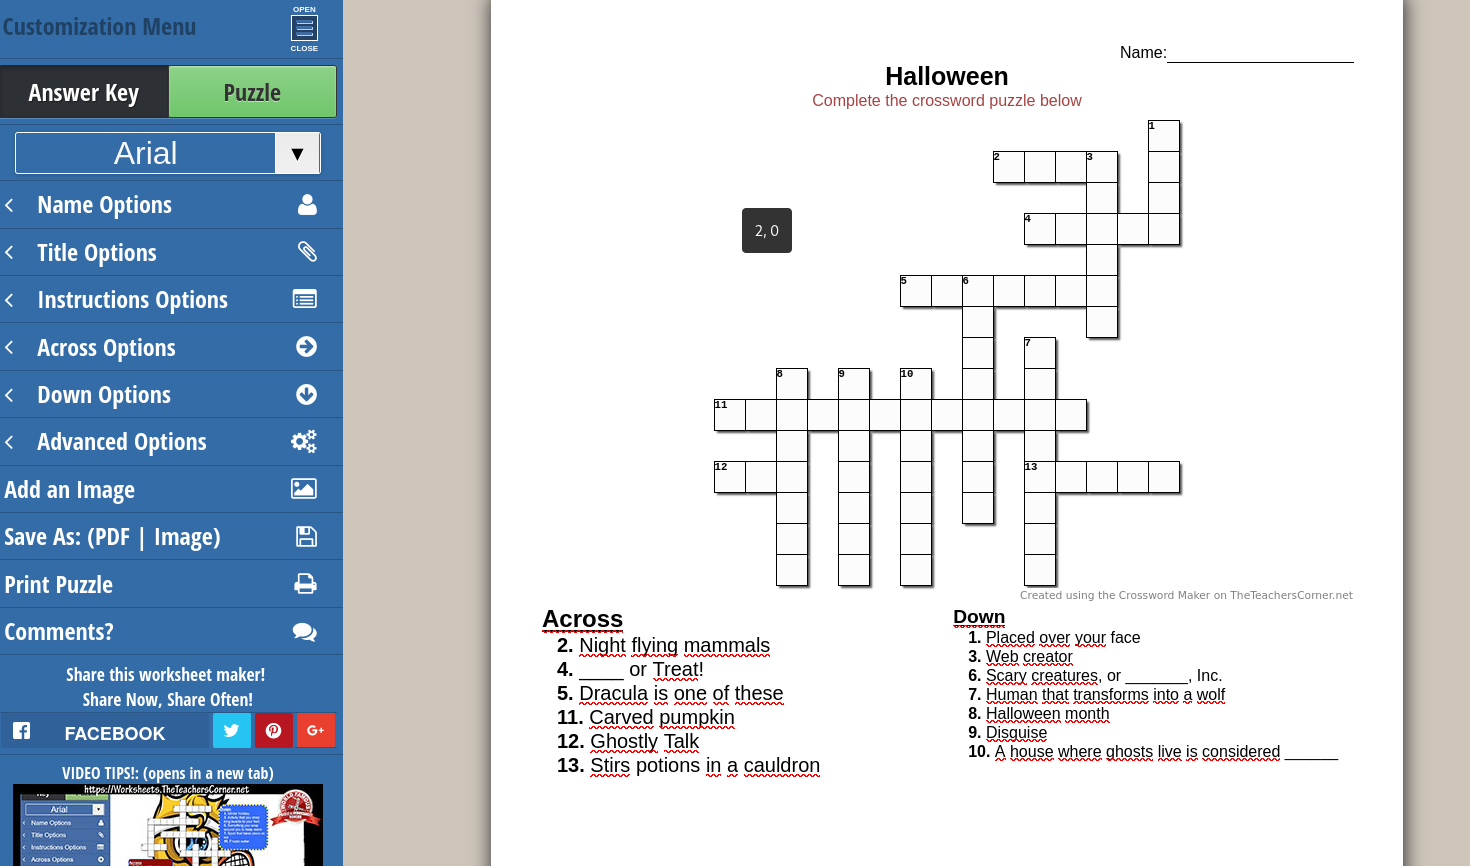
\includegraphics[scale=0.25]{theteachercorner.png}
                    \caption{Interface Application "The Teacher’s Corner : puzzle and activities" }
                    \label{Pres}
                \end{center}
            \end{figure}
        \end{center}
        
        \item Sport Cérébral : mots croisés \cite{McG}
        \\
        \\ Cet outil permet de remplir une unique grille chaque jour dans le but de se divertir. Il ne permet aucune option de génération ou d’exportation. Cependant dans les fonctionnalités on a accès à des boutons indices et des options ergonomiques tels que le zoom, la possibilité d’effacer nos mots, etc pour enfin valider notre grille. D’un point de vue design et besoins utilisateurs, cette application est en adéquation avec le projet.
        
        \begin{center}
            \begin{figure}[H]
                \begin{center}
                    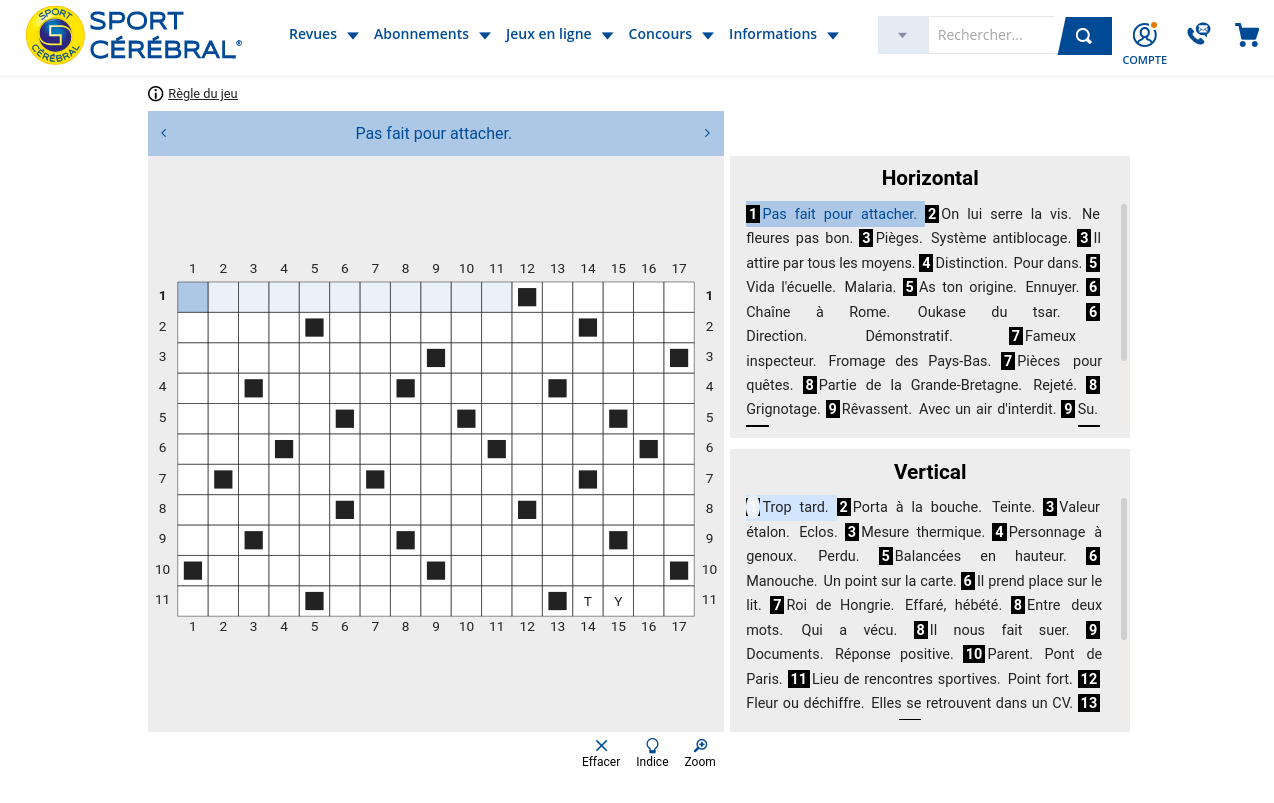
\includegraphics[scale=0.35]{sportcerebral.png}
                    \caption{Interface Application "Sport Cérébral : mots croisés" }
                    \label{Pres}
                \end{center}
            \end{figure}
        \end{center}
        
        \newpage
        \item Education.com : Crossword Puzzle \cite{Cp}
        \\
        \\ Outil permettant de générer ses propres mots croisés, avec une très légère option de personnalisation du design (bordures) et possibilité d’export/import de nos propres grilles.
        
        \begin{center}
            \begin{figure}[H]
                \begin{center}
                    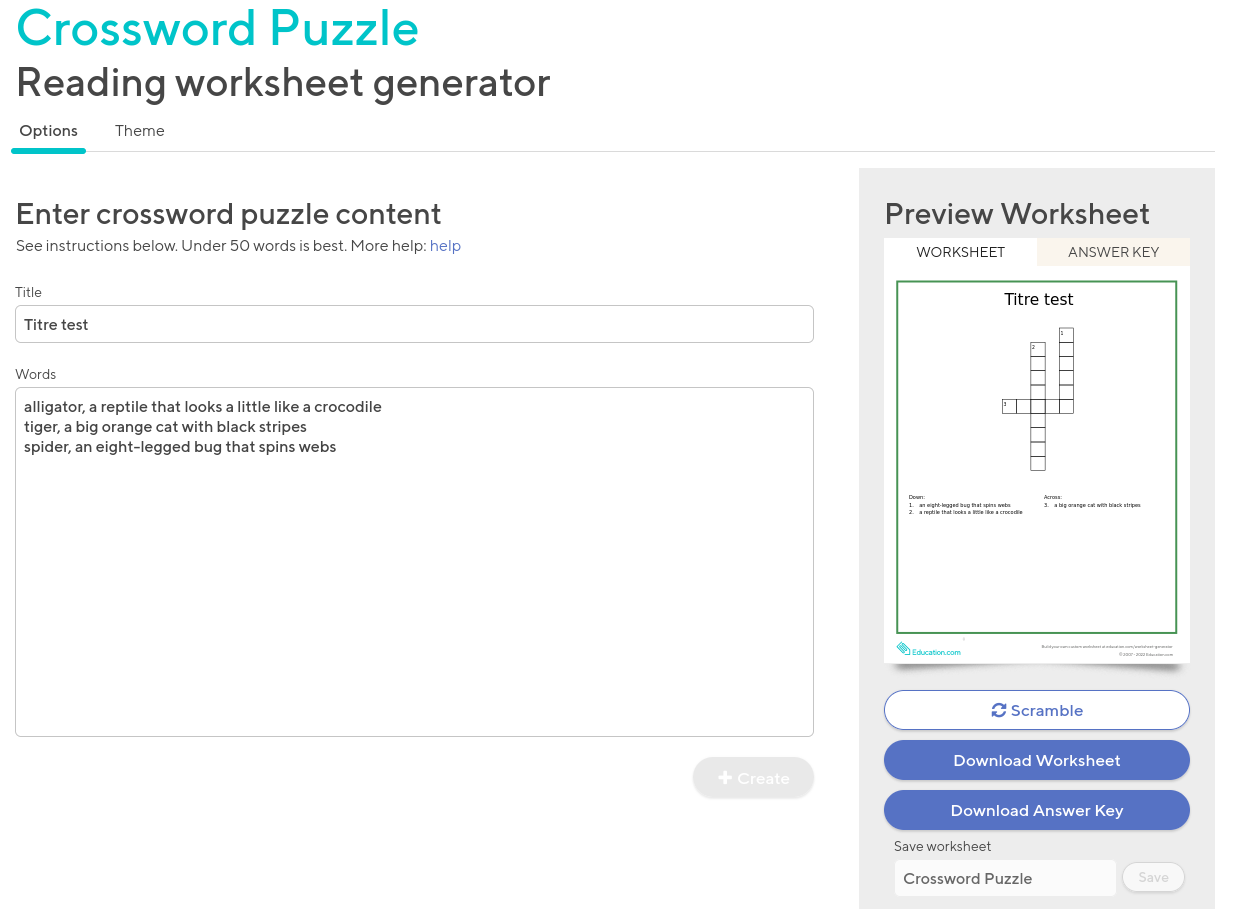
\includegraphics[scale=0.35]{education.png}
                    \caption{Interface Application "Education.com : Crossword Puzzle" }
                    \label{Pres}
                \end{center}
            \end{figure}
        \end{center}
        
        \newpage
        \item Puzzel \cite{Cc}
        \\ 
        \\ Outil à l’interface soignée, beaucoup d’options ne sont malheureusement accessibles qu’avec une participation financière.
        
        \begin{center}
            \begin{figure}[H]
                \begin{center}
                    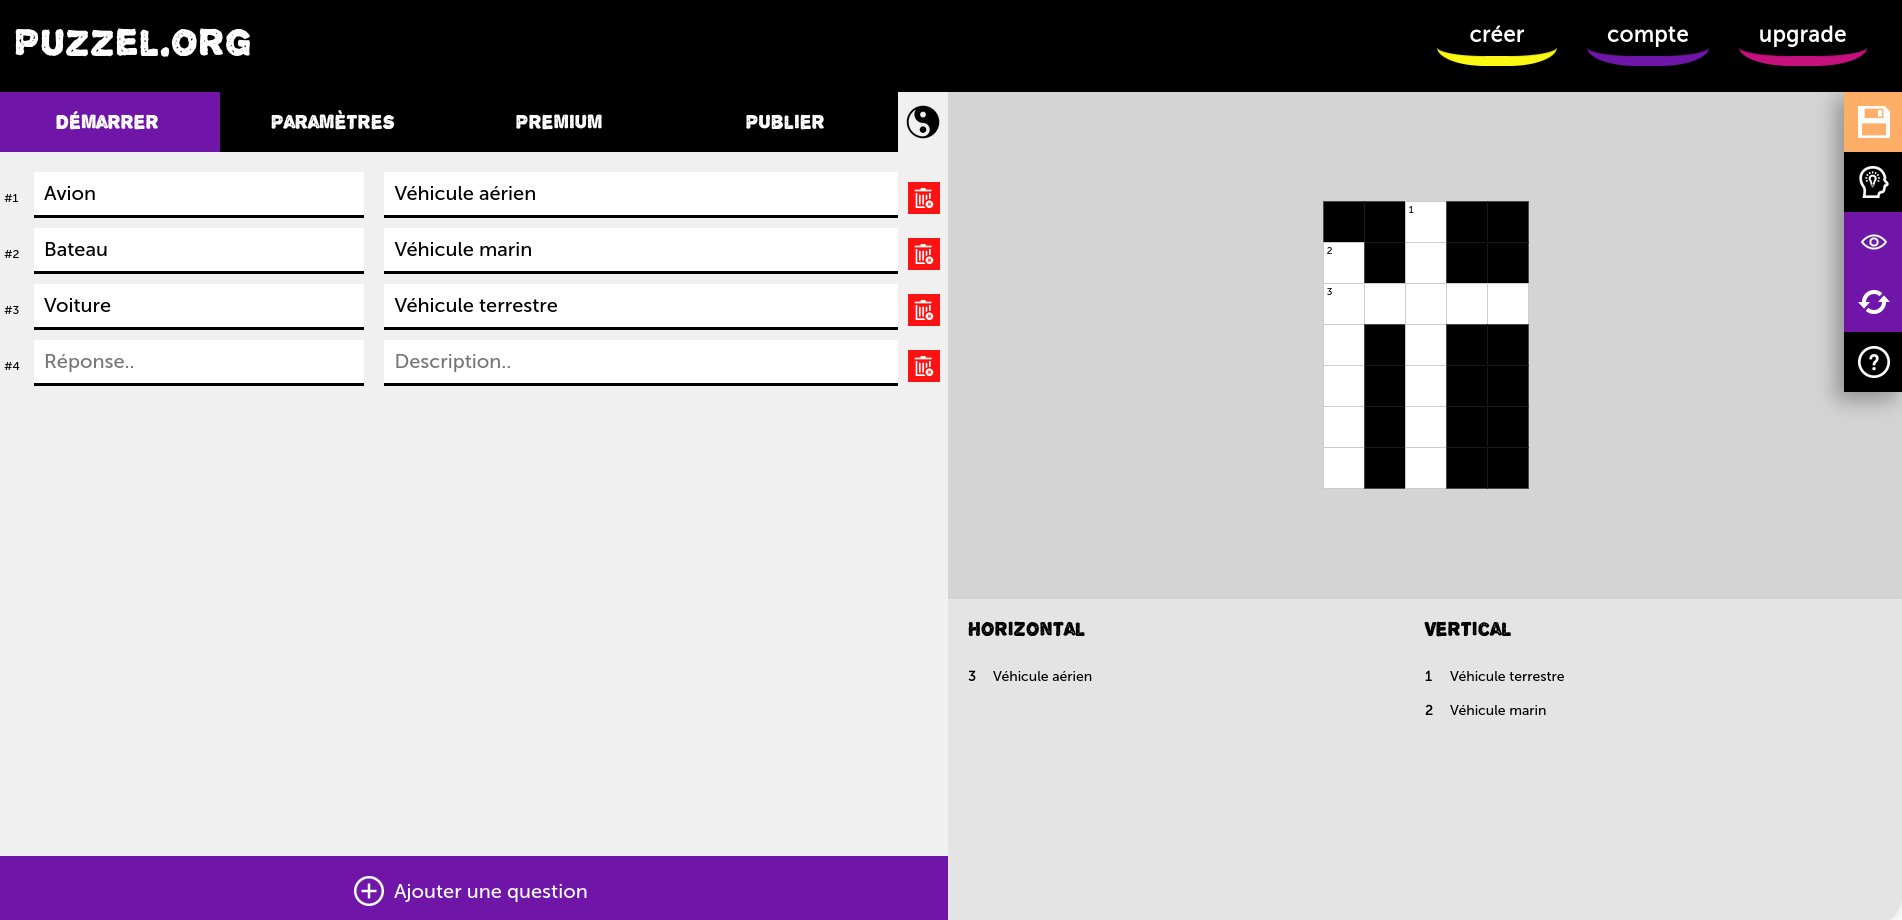
\includegraphics[scale=0.25]{puzzel.png}
                    \caption{Interface Application "Puzzel" }
                    \label{Pres}
                \end{center}
            \end{figure}
        \end{center}
    
    \end{itemize}
    
    \newpage
    \subsection{Logiciel nécessitant une installation}
    \begin{itemize}
        
         \item EclipseCrossword\cite{Ec}
        \\ Disponible sur le catalogue d'applications Microsoft. Ce logiciel est gratuit et disponible uniquement sur Windows.
        \\ Logiciel complet de création de grille.
        Possibilité d’importer une liste de mots/indices.
        Possibilité d’enregistrer sa grille dans le format du logiciel (.ecw) et sa “word list”, d’imprimer avec plusieurs options (présence des réponses dans la grille, afficher les indices, etc…) et partager sa grille en ligne.
        On trouve également des options plus avancées comme des exports html, rtf, wmf, eps et “across lite text format”.
        
        \begin{center}
            \begin{figure}[H]
                \begin{center}
                    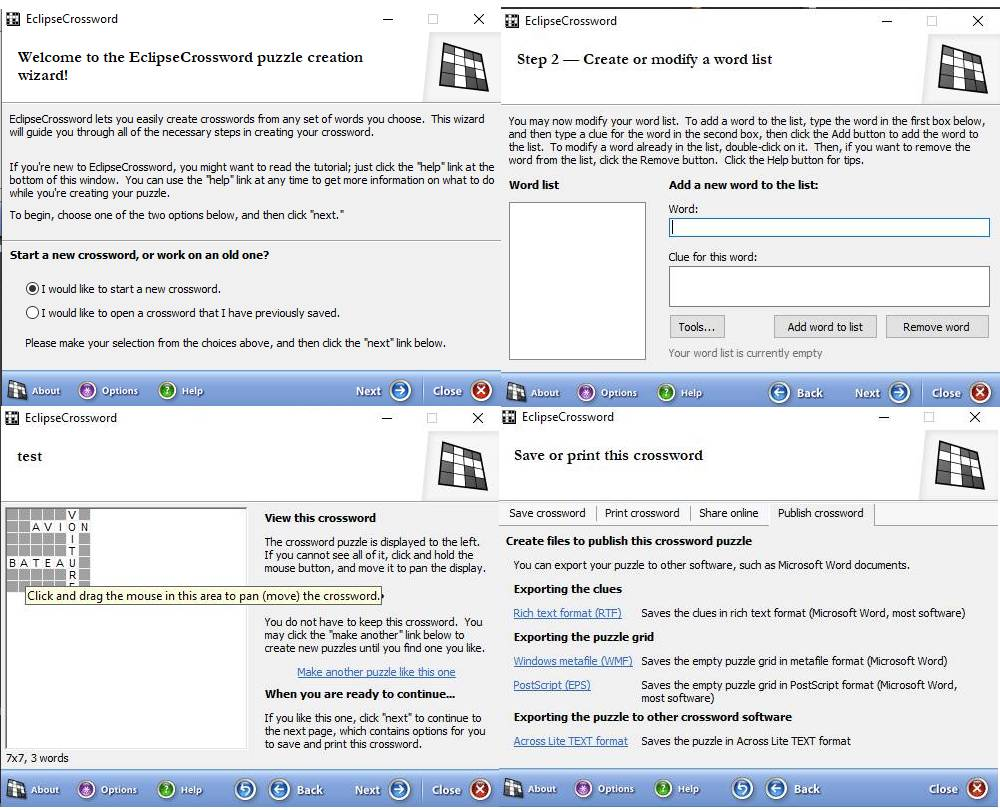
\includegraphics[scale=0.55]{eclipsecrossword.jpg}
                    \caption{Interface Application "Eclipse Crossword" }
                    \label{Pres}
                \end{center}
            \end{figure}
        \end{center}
        
         \item Mots-croisés-Pro \cite{At}
        \\ 
        \\ Logiciel payant disponible uniquement sur Windows au prix de 59 euros. Une version gratuite d’essai est disponible.
        \\ Ce logiciel permet la création de grilles de mots croisés ou fléchés jusqu'à 400 cases. Il permet de créer des grilles de manière automatique, semi-automatique ou manuelle.
        Outil extrêmement complet, mais malheureusement limité dans sa version gratuite.
        
        \begin{center}
            \begin{figure}[H]
                \begin{center}
                    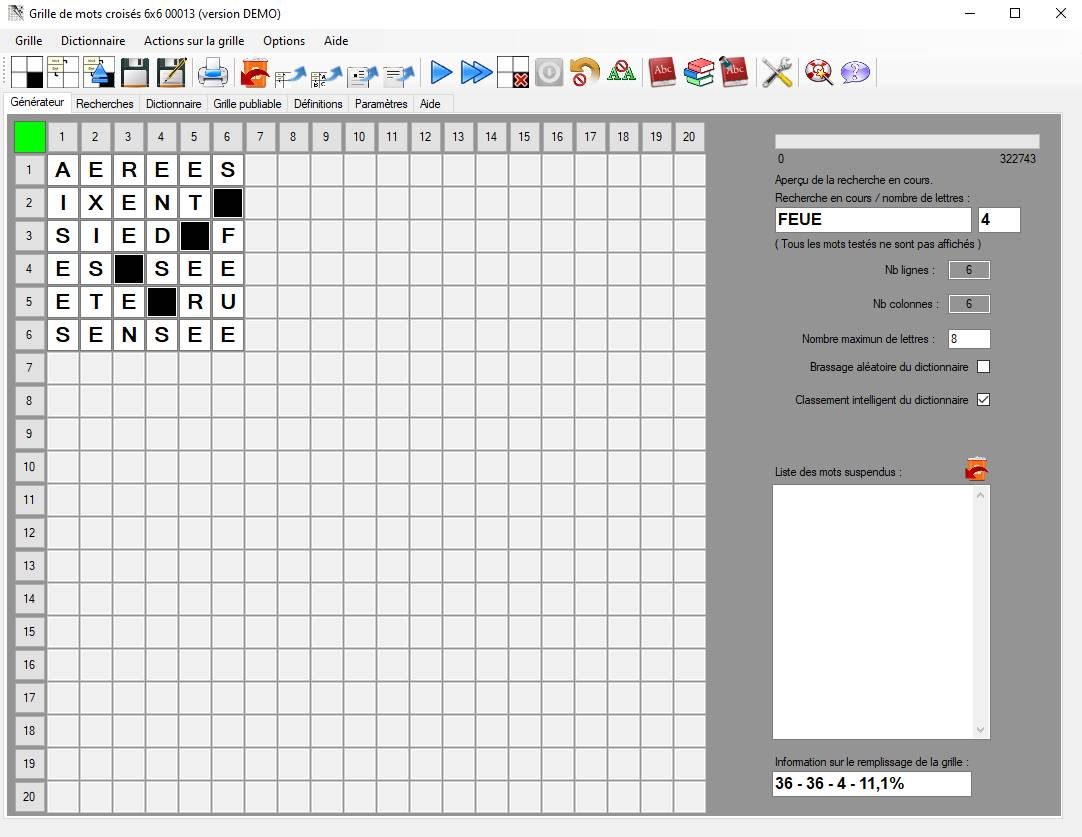
\includegraphics[scale=0.45]{mots croises pro.jpg}
                    \caption{Interface Application "Mots croisés pro" }
                    \label{Pres}
                \end{center}
            \end{figure}
        \end{center}
    
    \end{itemize}
        

    \subsection{Synthèse}
        \hspace{1cm}La plupart des générateurs facilement trouvables en ligne permettent de créer des grilles très simples, la cible de ces générateurs sont probablement des enfants ou un public non expert des mots-croisés, l’utilisation de tels outils semble adaptée à un but éducatif. En revanche aucun des ces outils ne semble proposer de solutions plus avancées telles que l’on pourrait trouver dans des journaux ou magazines spécialisés. En effet si l’on cherche à construire une grille complexe avec peu de cases noires (absence de lettres) et des normes précises comme une taille de grille particulière ou le respect de la symétrie (voir figure plus bas), il faut nous pencher vers des logiciels plus avancés et souvent payants, comme le fait Mots-croisés-Pro. De plus ces logiciels sont davantage une aide à la construction manuelle de grille, qu’une solution toute faite automatisée.\\
        
        \hspace{1cm}Dans notre application, les options de personnalisation poussées ne seront pas prioritaires, elles viendront enrichir notre logiciel que dans un second temps.
        Nous voulons nous inspirer des options d’aide à la résolution de grille pour l’utilisateur comme ceux présents dans Sport Cérébral par exemple.
        Nous ne prévoyons pas d’utiliser le web pour notre application (pour ne pas nous préoccuper des conventions du web telles que les requêtes HTTP), ainsi l’interface utilisateur devrait être bien différente des générateurs en ligne que l’on a pu étudier ici. Le partage et la publication de grilles ne nous concerne pas particulièrement, les options d’imports/exports à l’usage d’un seul utilisateur nous suffisent.

\newpage
\section{Besoins fonctionnels} %(C + E)
\subsection{Avant-propos} %parler de E C O

 Nous utiliserons les codes de correspondance suivants au sein des besoins :
    \begin{itemize}
        \item \textbf{(E)} : Essentiel $\rightarrow$ le logiciel ne sera pas acceptable sans que ce besoin soit réalisé.
        \item \textbf{(C)} : Conditionnel $\rightarrow$ besoin qui étend et améliore le logiciel, sans que ce besoin soit nécessaire pour rendre le logiciel acceptable.
        \item \textbf{(O)} : Optionnel $\rightarrow$ besoin dont la valeur n'est pas encore assurée.
    \end{itemize}
Pour chacun des besoins présentés, nous écrirons ici 3 différents tests : 
    \begin{itemize}
        \item test \textbf{positif} (ou test d'affirmation) qui vérifie le bon fonctionnement du besoin dans des conditions d'utilisation correctes (qui ne "stressent" pas les cas d'utilisation du logiciel). 
        
        \item test \textbf{négatif} qui vérifie le comportement hors des cas d'utilisation définis par les besoins du logiciel.
        
        \item test \textbf{aux frontières}, ils s'appliquent aux limites/frontières de fonctionnement normal. Ils sont donc situés à la frontière entre les cas d'utilisation entraînant un test positif, et ceux entraînant un test négatif. A noter que ce test ne peut pas s'appliquer à tous les besoins, nous ne le mettrons donc pas toujours (comme parfois les tests négatifs).
    \end{itemize}      
Pour chacun des tests énoncés ci-après, nous énoncerons d'abord le nom du besoin tel qu'exprimé précisemment dans le cahier des besoins, puis nous écrirons les 3 tests selon l'ordre expliqué en introduction. Nous séparerons chacun des 3 tests selon la charge graphique suivante : fond bleu = test positif / fond rouge = test négatif / fond gris = test aux frontières. A noter que sur certains besoins, nous n'avons pas trouvé de tests négatifs et aux frontières pertinents. \newline

\subsection{Diagramme des cas d'utilisation} %(Y)
\begin{center}
    \begin{figure}[!ht]
        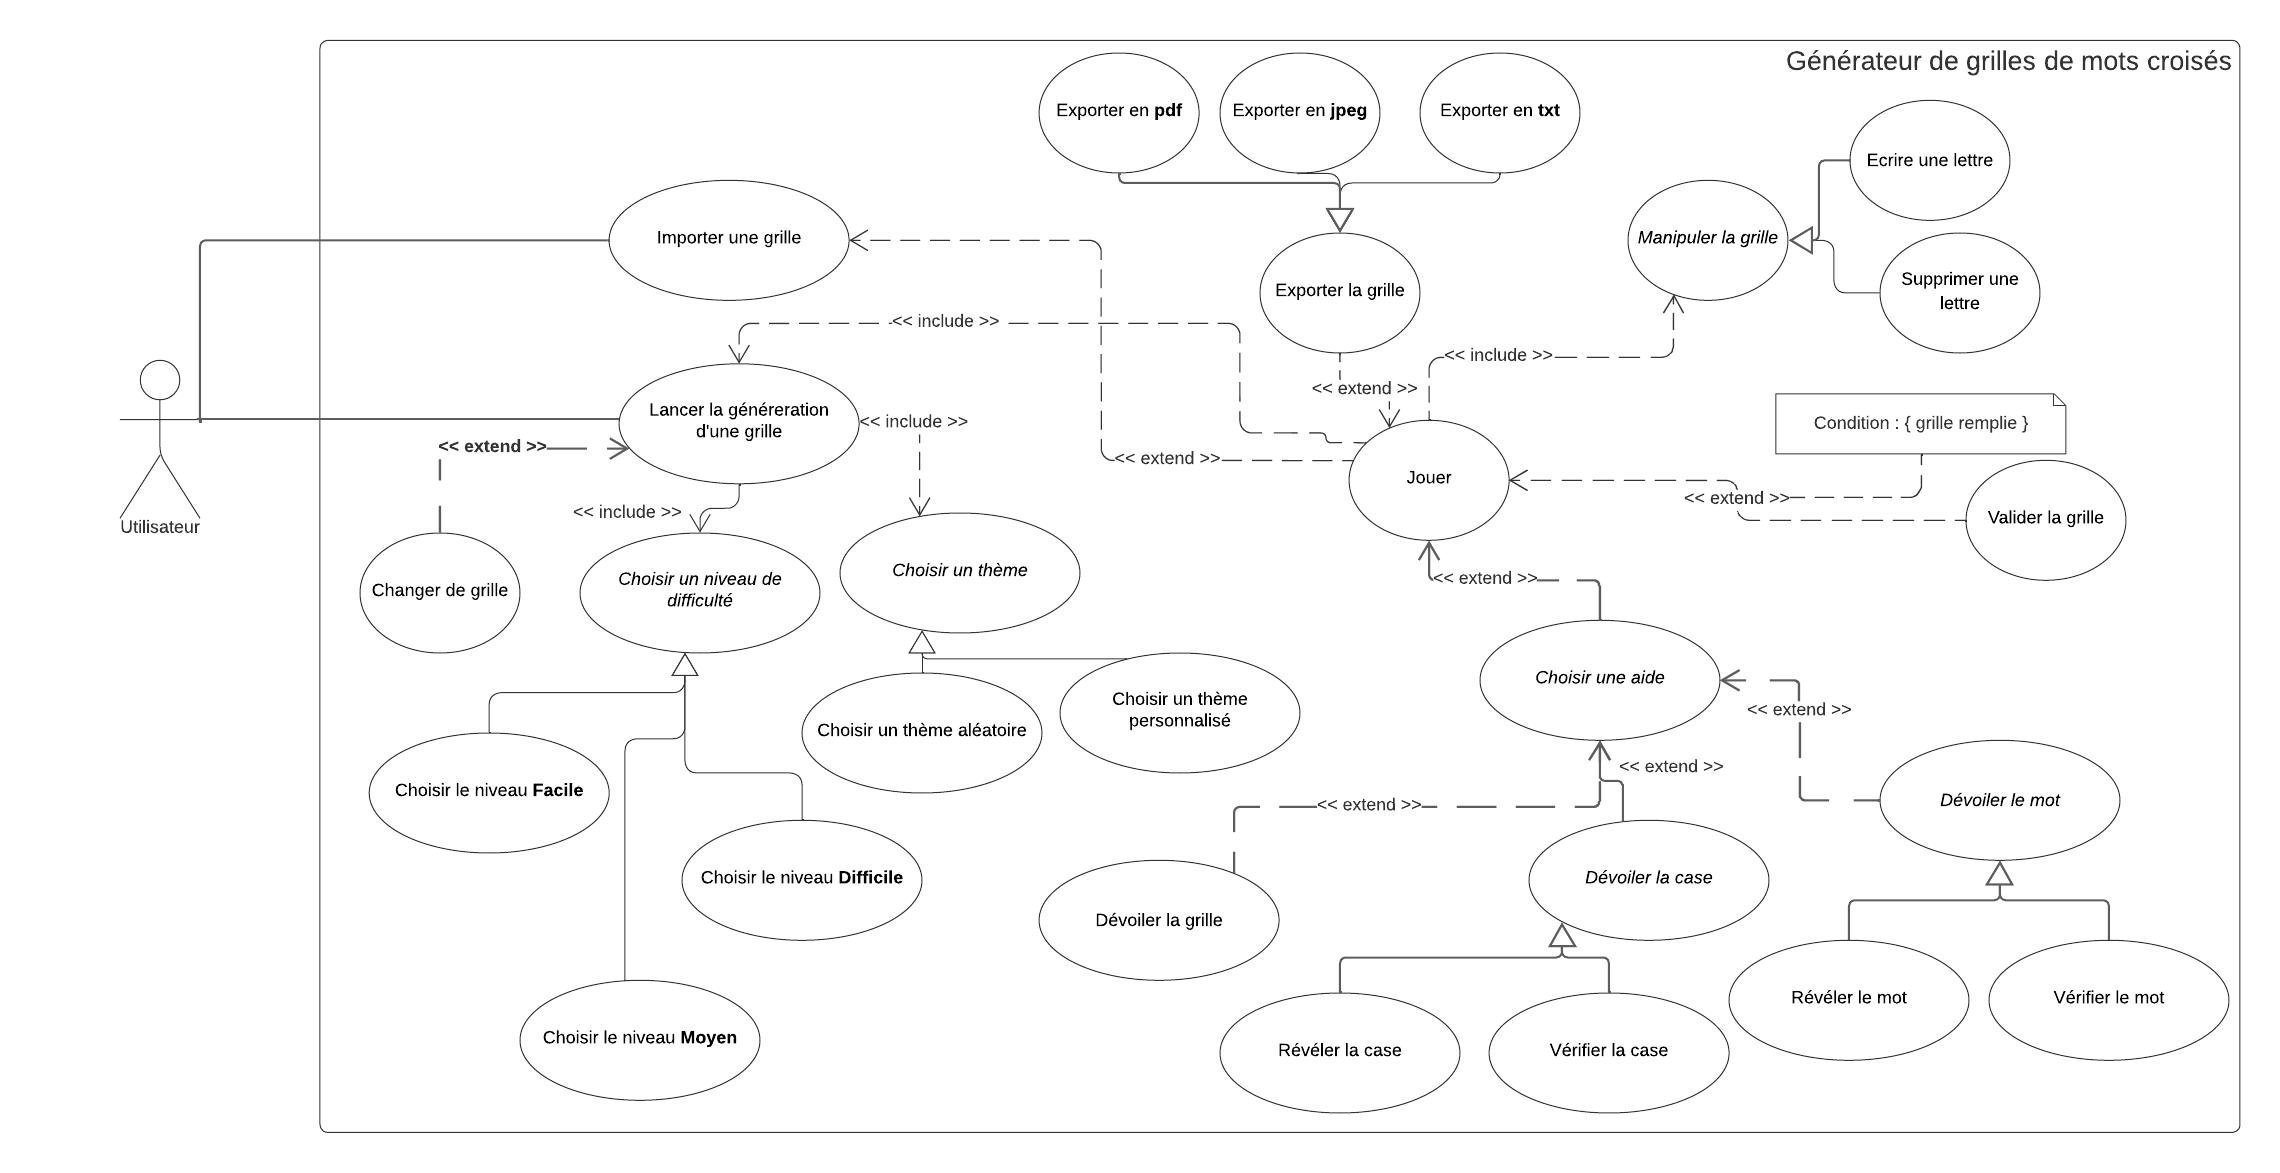
\includegraphics[height=3in, width=\textwidth]{DCU.png}
        \caption{Diagramme de cas d'utilisation} 
    \end{figure}
\end{center}

\noindent{Le besoin principal de notre application est naturellement de pouvoir générer une grille en y appliquant un niveau de difficulté et de permettre à l’utilisateur d’y jouer. Aussi, l’utilisateur doit impérativement pouvoir bénéficier d’aides diverses l’aidant à la résolution de la grille, il pourra réveler ou vérifier une case ou un mot ou dévoiler la grille entièrement. Lorsque la grille est remplie il pourra valider ses réponses. Il est enfin important dans notre application que l’on puisse arrêter à tout moment une partie en cours et pouvoir la reprendre quand l'utilisateur le souhaite : import et export d'une grille. C’est d’ailleurs un des points qui nous a semblé manquant sur l’existant étudié.}

\subsection{Besoins utilisateurs}

{\color{blue}\textbf{(O) Importer une grille}} \\ \\ %(Définir le format txt d'une grille)
\underline {Acteur} : Utilisateur. \\
\underline {Résumé} : L'utilisateur souhaite importer une grille spécifique sur l'application pour y jouer. \\
\underline {Préconditions} : L'application est correctement lancée. \\
\underline {Post conditions} : L'utilisateur peut jouer sur la grille qu'il a importée. \\\\
\underline {Enchaînement nominal} : 
\begin{table}[H]
\centering
\begin{tabular}{|c|c|c|c|}
\hline
\textbf{Étapes} &
  \textbf{Utilisateur} &
  \textbf{Système}&
  \textbf{Maquette correspondante} \\ \hline
1 &
  \begin{tabular}[c]{@{}c@{}}Clique sur\\ "File/Import"\end{tabular} & & Maquette - Accueil
   \\ \hline
2 &
  \begin{tabular}[c]{@{}c@{}}Sélectionne le fichier\\ correspondant \end{tabular} & & \begin{tabular}[c]{@{}c@{}}Maquette - \\Menu d'importation\end{tabular}
   \\ \hline
3 &
   &
   \begin{tabular}[c]{@{}c@{}}Vérifie la validité du\\ fichier\\ (cf. codage d'une grille)\end{tabular} & / \\ \hline
4 &
   &
  \begin{tabular}[c]{@{}c@{}}Affiche la grille ou une erreur\\ d'importation\end{tabular}& \begin{tabular}[c]{@{}c@{}}Maquette - \\Grille précemment remplie importée \end{tabular}\\ \hline
\end{tabular}
\end{table} 

    \begin{figure}[H]
    \begin{center}
        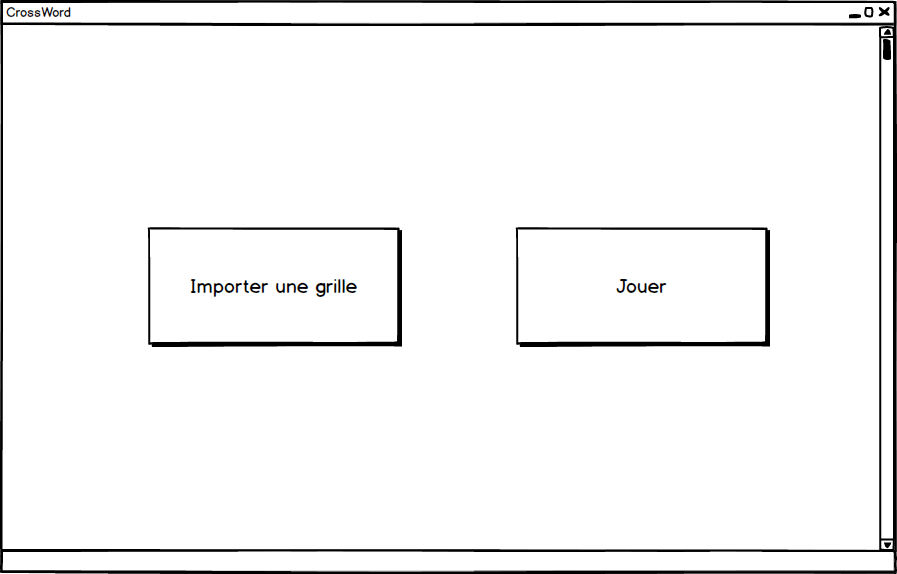
\includegraphics[height=3in]{Maquettes/Accueil.png}
        \caption{Maquette - Accueil} 
        \end{center}
    \end{figure}
    
        \begin{figure}[H]
    \begin{center}
        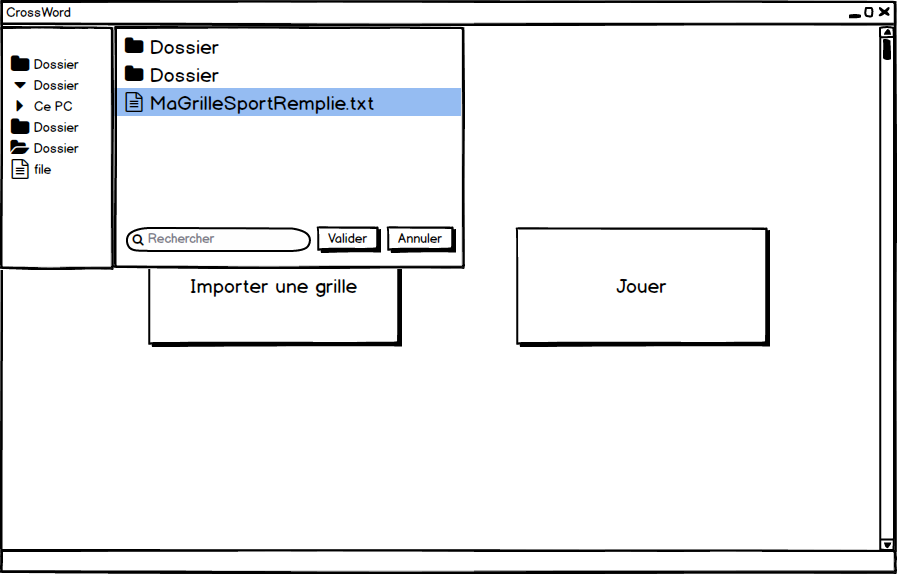
\includegraphics[height=3in]{Maquettes/Import.png}
        \caption{Maquette - Menu d'importation} 
        \end{center}
    \end{figure}
    
        \begin{figure}[H]
    \begin{center}
        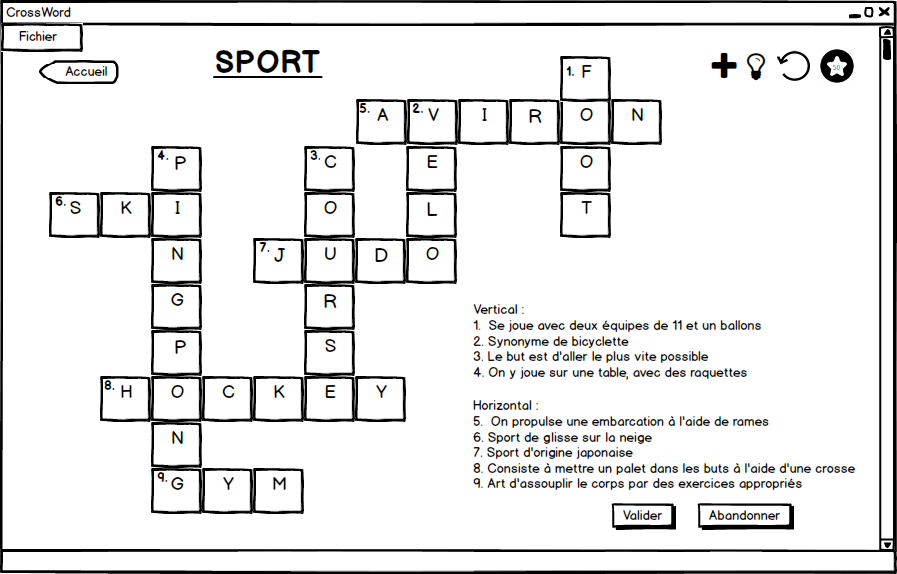
\includegraphics[height=3in]{Maquettes/Grille_remplie.png}
        \caption{Maquette - Grille précemment remplie importée} 
        \end{center}
    \end{figure}



\noindent{\underline {Codage d'une grille}} : La grille sera codée dans un fichier .txt, nous devrons stocker les différents mots et définitions pour que le système arrive à regénerer correctement la grille.
Le format précis du codage sera précisé lors des spécifications techniques, si le fichier .txt ne respecte pas le codage, le système retournera une erreur lors de l'importation.\\ \\

\newpage
\noindent{\underline {Tests associés}} : 
\begin{tcolorbox}[colback=positifC]
            \begin{enumerate}
                \item \textit{Description et but du test }: Importation d'une sauvegarde valide d'une grille.
                
                \item \textit{Cas de test }: On utilise la sauvegarde d'un grille "témoin" valide. On importe cette grille sauvegardée et on vérifie que l'importation de cette derniere a bien été effectuée.
                
                \item \textit{Déroulement et scénario du test }: On sauvegarde une grille sur notre machine, on l'importe et on vérifie que la grille importée est la même que la grille fraichement sauvegardée.
                
                \item \textit{Analyse du test }: Si la grille  importée est bien celle attendu alors le test est valide, invalide sinon.
            \end{enumerate}
        \end{tcolorbox}
        
        \begin{tcolorbox}[colback=negatifC]
            \begin{enumerate}
                \item \textit{Description et but du test }: Importation d'une sauvegarde non valide d'une grille (format de fichier non conforme). 
                
                \item \textit{Cas de test }: Un fichier de sauvegarde invalide d'une grille. Il est attendu que le logiciel ne se charge pas et qu'un message d'erreur s'affiche.
                
                \item \textit{Déroulement et scénario du test }: On importe la sauvegarde invalide dans notre logiciel avec l'aide du bouton "Importer une grille".
                
                \item \textit{Analyse du test }: Si un message d'erreur indiquant que le fichier est invalide s'affiche alors le test est valide, sinon il est échoué.
            \end{enumerate}
        \end{tcolorbox}


\newpage
\noindent{{\color{blue}\textbf{(E) Choisir un niveau de difficulté }}} \\ \\ %(Définir les différentes difficultés)
\underline {Acteur} : Utilisateur. \\
\underline {Résumé} : L'utilisateur peut choisir une difficulté pour la grille de mots croisés (il se rend dans "play/select difficulty/difficuly wanted). \\
\underline {Préconditions} : L'application est correctement lancée et l'utilisateur a choisi de commencer à jouer. \\
\underline {Post conditions} : L'utilisateur a la liberté de jouer selon différentes difficultés. \\\\
\underline {Maquette} : \\% ~ un seule action donc une maquette pour décrire suffit je pense

    \begin{figure}[H]
    \begin{center}
        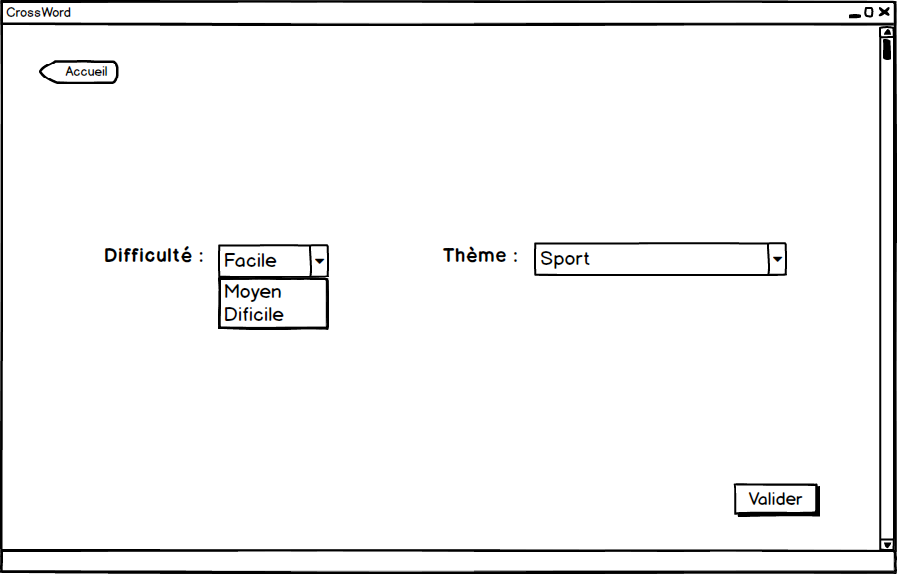
\includegraphics[height=3in]{Maquettes/ChoixDiff_deroule.png}
        \caption{Maquette - Choix de la difficulté} 
        \end{center}
    \end{figure}

\noindent{\underline {Les différentes difficultés}} :  La difficulté d'une grille sera définie par la taille de la grille et le nombre d'aides autorisées au joueur. Nous aurons 3 niveaux de difficultés : Facile (grille 6x6), Moyen (grille 8x8) et Difficile (grille 10x10). \\ \\
\noindent{\underline {Test associé}} : 
 \begin{tcolorbox}[colback=positifC]
            \begin{enumerate}
                \item \textit{Description et but du test }: Vérifier que la génération des grilles est bien modifiée en fonction du niveau de difficulté.

                
                \item \textit{Cas de test }: Utilisation du logiciel témoin (sans condition de stress). Le résultat attendu est que la grille soit générée avec la méthode qui représente la difficulté sélectionnée.
                
                \item \textit{Déroulement et scénario du test }: On génère la grille avec chaque difficulté possible, à chaque génération on vérifie que la grille sélectionnée est générée avec la méthode reliée correspondant à sa difficulté.
                
                \item \textit{Analyse du test }: Si chaque grille a été générée avec la méthode correspondant à son niveau de difficulté alors le test est validé sinon il a échoué.
            \end{enumerate}
        \end{tcolorbox}
        

\newpage
\noindent{{\color{blue}\textbf{(O) Choisir un thème}}} \\ \\% ~ Maquette à changer
\underline {Acteur} : Utilisateur. \\
\underline {Résumé} : L'utilisateur peut choisir un thème pour la grille de mots croisés. \\
\underline {Préconditions} : L'application est correctement lancée et l'utilisateur à choisi de commencer à jouer. \\
\underline {Post conditions} : L'utilisateur a la liberté de jouer sur des grilles de différents thèmes. \\\\
\underline {Maquette} : \\% ~ un seule action donc une maquette pour décrire suffit je pense

    \begin{figure}[H]
    \begin{center}
        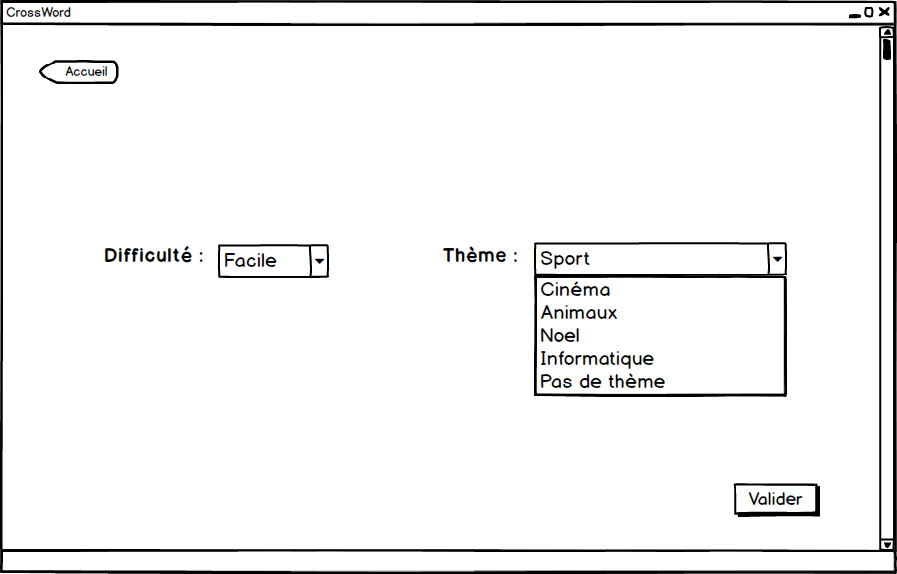
\includegraphics[height=3in]{Maquettes/ChoixTheme_deroule.png}
        \caption{Maquette - Choix du thème} 
        \end{center}
    \end{figure}


\noindent{\underline {Les différents thèmes}} : Les thèmes influenceront les mots qui composent la grille, par exemple un thème de sport donnera une grille avec des mots du lexique du sport. Les thèmes auxquels nous avons pensé sont : Sport, Cinéma, Animaux, Noël, Informatique. \\ \\
\noindent{\underline {Test associé}} : 
 \begin{tcolorbox}[colback=positifC]
            \begin{enumerate}
                \item \textit{Description et but du test }: Vérifier que les mots utilisés pour créer la grille viennent de la liste de mots correspondant au théme.
                
                \item \textit{Cas de test }: Utilisation du logiciel témoin (sans condition de stress) et des listes de mots des différents thèmes. On s'attendait à ce que les grilles générées avec un thème  n'utilisent que des mots de la liste de son thème.
                
                
                \item \textit{Déroulement et scénario du test }: On génère la grille avec chaque thème et pour chaque grille on vérifie que seuls les mots de leurs thèmes ne composent la grille. 
                
                \item \textit{Analyse du test }: Si chaque grille n'est composée que des mots correspondant à son thème alors le test est validé, sinon le test échoue.

            \end{enumerate}
        \end{tcolorbox}


\newpage
{\color{blue}\textbf{(C) Changer de grille}} \\ \\
\underline {Acteur} : Utilisateur. \\
\underline {Résumé} : L'utilisateur n'est pas satisfait d'une grille et veut donc changer de grille. \\
\underline {Préconditions} : L'application est correctement lancée, l'utilisateur est en train de jouer sur une grille. \\
\underline {Post conditions} : La nouvelle grille est affichée, l'utilisateur peut maintenant jouer. \\\\
\underline {Enchaînement nominal} : 
\begin{table}[H]
\centering
\begin{tabular}{|c|c|c|c|}
\hline
\textbf{Étapes} &
  \textbf{Utilisateur} &
  \textbf{Système}  &
  \textbf{Maquette correspondante} \\ \hline
1 &
  \begin{tabular}[c]{@{}c@{}}Clique sur\\ "Changer de grille"\end{tabular} & & (Bouton + de l'écran de jeu)
   \\ \hline
2 &
   & Affiche les différentes options & \begin{tabular}[c]{@{}c@{}}Maquette - \\Paramétrage de la grille\end{tabular}  \\ \hline
3 & \begin{tabular}[c]{@{}c@{}}Choisi une difficulté\\ (cf. "Choisir une difficulté")\end{tabular} & & (cf. "Choisir une difficulté") {\color[HTML]{000000} \textbf{}} \\ \hline
4 &
  \begin{tabular}[c]{@{}c@{}}Choisi un thème\\ (cf. "Choisir un thème")\end{tabular} & & (cf. "Choisir un thème")
   \\ \hline
5 &
  Valide sa sélection & & \begin{tabular}[c]{@{}c@{}}Maquette -\\ Paramétrage de la grille\end{tabular} 
   \\ \hline
6 &
   &
  \begin{tabular}[c]{@{}c@{}}Génère la grille\end{tabular} & /\\ \hline
7 &
   &
  Affiche la grille & Maquette - Grille vide \\ \hline
\end{tabular}
\end{table}
    
    \begin{figure}[H]
    \begin{center}
        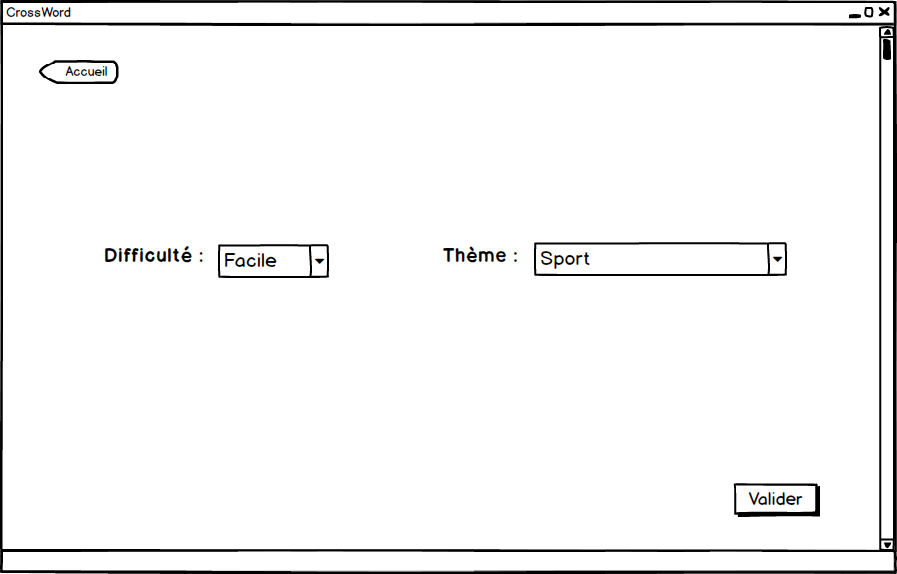
\includegraphics[height=3in]{Maquettes/ChoixThemeDifficulte.png}
        \caption{Maquette - Paramétrage de la grille} 
    \end{center}
    \end{figure}

    \begin{figure}[H]
    \begin{center}
        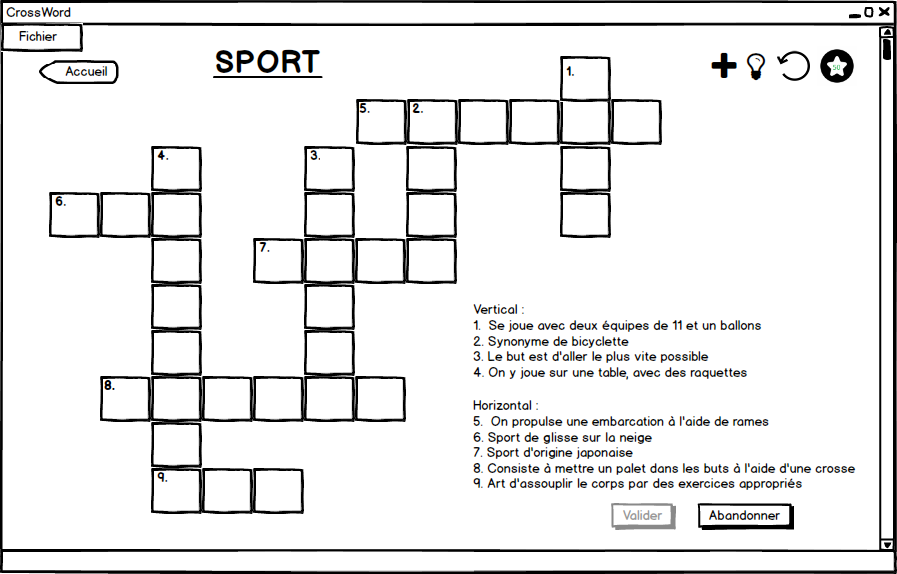
\includegraphics[height=3in]{Maquettes/Grille_vide.png}
        \caption{Maquette - Grille vide} 
    \end{center}
    \end{figure}


\noindent{\underline {Tests associés}} : 
\begin{tcolorbox}[colback=positifC]
            \begin{enumerate}
                \item \textit{Description et but du test }: Vérification que le bouton changer de grille génère bien une nouvelle grille.
                
                \item \textit{Cas de test }: Utilisation du logiciel témoin (sans condition de stress) . On s'attend à ce que le logiciel génére une nouvelle grille.
                
                
                \item \textit{Déroulement et scénario du test }: On clique sur le bouton "Changer de grille".
                
                \item \textit{Analyse du test }: On génère une nouvelle grille. On vérifie que cette dernière n'est composée que de mots appartennant au théme de l'ancienne grille. 

            \end{enumerate}
        \end{tcolorbox}
        \begin{tcolorbox}[colback=negatifC]
            \begin{enumerate}
                \item \textit{Description et but du test }: Vérification que le bouton changer de grille n'est pas disponible si aucune grille n'est génerée.
                
                \item \textit{Cas de test }: Utilisation du logiciel témoin (sans condition de stress) . On s'attend à ce que le bouton de changement de grille ne soit pas affiché.
                
                
                \item \textit{Déroulement et scénario du test }: On lance l'application et on vérifie que le bouton n'est pas présent.
                
                \item \textit{Analyse du test }: Le test est un succès si le bouton n'est pas affiché.

            \end{enumerate}
        \end{tcolorbox}


\newpage
\noindent{{\color{blue}\textbf{(E) Lancer la géneration d'une grille}}} \\ \\
\underline {Acteur} : Utilisateur. \\
\underline {Résumé} : L'utilisateur lance la génération d'une grille de mots croisés en vue d'y jouer (detaillé sur le PDF Algorithmes, choix techniques, outils utilisés). \\
\underline {Préconditions} : L'application est correctement lancée. \\
\underline {Post conditions} : La grille est affichée, l'utilisateur peut maintenant jouer. \\\\
\underline {Enchaînement nominal} : 
\begin{table}[H]
\centering
\begin{tabular}{|c|c|c|c|}
\hline
\textbf{Étapes} &
  \textbf{Utilisateur} &
  \textbf{Système} &
  \textbf{Maquette correspondante} \\ \hline
1 &
  \begin{tabular}[c]{@{}c@{}}Clique sur\\ "Jouer"\end{tabular} & & (cf. Maquette - Accueil)
   \\ \hline
2 &
   &
  Affiche les différentes options & \begin{tabular}[c]{@{}c@{}}(cf. Maquette - \\Paramétrage de la grille) \end{tabular}  \\ \hline
3 & \begin{tabular}[c]{@{}c@{}}Choisit une difficulté\\ (cf. "Choisir une difficulté")\end{tabular} & & (cf. "Choisir une difficulté"){\color[HTML]{000000} \textbf{}} \\ \hline
4 &
  \begin{tabular}[c]{@{}c@{}}Choisit un thème\\ (cf. "Choisir un thème")\end{tabular} & & (cf. "Choisir un thème")
   \\ \hline
5 &
  Valide sa sélection & & \begin{tabular}[c]{@{}c@{}}(cf. Maquette - \\Paramétrage de la grille)\end{tabular} 
   \\ \hline
6 &
   &
  \begin{tabular}[c]{@{}c@{}}Génère la grille\\ \end{tabular} & /\\ \hline
7 &
   &
  Affiche la grille & (cf. Maquette - Grille vide) \\ \hline
\end{tabular}
\end{table}

\noindent{\underline {Test associé}} :
        \begin{tcolorbox}[colback=positifC]
            \begin{enumerate}
                \item \textit{Description et but du test }: Vérifier que la génération de la grille fonctionne.
 
                
                \item \textit{Cas de test }: Génération de la grille en fonction du thème et de la difficulté choisie par l'utilisateur.
                
                \item \textit{Déroulement et scénario du test }: Seléction d'un thème et d'une difficulté, valider la sélection.
                
                \item \textit{Analyse du test }: Vérifier que la grille est bien solvable par l'utilisation de notre solveur. Vérification de la bonne appartenance des mots de la grille au thème et à la difficulté seléctionnée préalablement. 
            \end{enumerate}
        \end{tcolorbox}


\newpage
\noindent{{\color{blue}\textbf{ (E) Jouer (remplir les cases)}}} \\ \\
\underline {Acteur} : Utilisateur. \\
\underline {Résumé} : L'utilisateur veut jouer à une grille de mots croisés. \\
\underline {Préconditions} : L'application est correctement lancée. \\
\underline {Post conditions} : La grille est affichée, l'utilisateur peut maintenant jouer. \\\\
\underline {Enchaînement nominal} : 
\begin{table}[H]
\centering
\begin{tabular}{|c|c|c|c|}
\hline
\textbf{Étapes} & \textbf{Utilisateur} & \textbf{Système}  &   \textbf{Maquette correspondante} \\ \hline
1                 & Sélectionne une case &  & (cf. Maquette - Grille vide) \\ \hline
2                 &                      & \begin{tabular}[c]{@{}c@{}}Prend en compte la case\\ sélectionnée\end{tabular} &  (cf. Maquette - Grille vide)\\ \hline
3 & \begin{tabular}[c]{@{}c@{}}Rentre une nouvelle\\ valeur (au clavier)\end{tabular} & & / {\color[HTML]{000000} \textbf{}} \\ \hline
4                 &                      & \begin{tabular}[c]{@{}c@{}}Affiche la nouvelle valeur de\\ la case\end{tabular}& Maquette - Partie en cours\\ \hline
\end{tabular}
\end{table}

   \begin{figure}[H]
    \begin{center}
        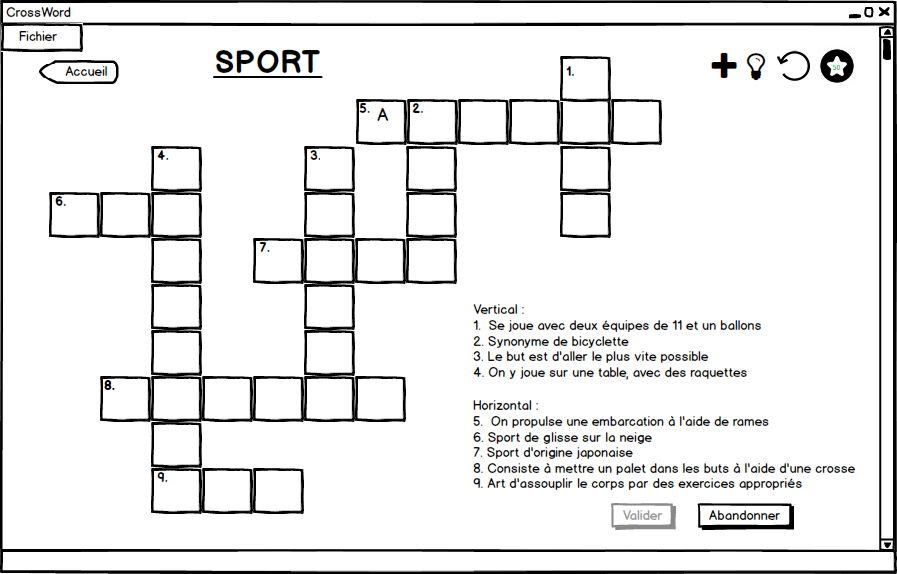
\includegraphics[height=3in]{Maquettes/Jouer.png}
        \caption{Maquette - Partie en cours} 
    \end{center}
    \end{figure}

\newpage
\noindent{\underline {Test associé}} :
\begin{tcolorbox}[colback=positifC]
            \begin{enumerate}
                \item \textit{Description et but du test} : L'utilisateur doit pouvoir remplir les cases de la grille par des lettres $ \in [a-zA-Z]$.\newline
                
                \item \textit{Cas de test} : Ecrire dans une case avec différents caractères. \newline
                
                \item \textit{Déroulement et scénario du test} : A partir d'une nouvelle grille, essayer de remplir des cases avec des caractères acceptés par le programme et par des caractères spéciaux ou majuscules (non acceptés)  \newline
                
                \item \textit{Analyse du test} : Verifier que les caractères spéciaux et majuscules ne sont pas entrés dans la case seléctionnée.  Seuls les caractères $\in[a-zA-Z]$ seront acceptés.
            \end{enumerate}
        \end{tcolorbox}


\newpage
\noindent{{\color{blue}\textbf{(O) Exporter la grille}}} \\ \\ %(Justifier les différents formats)
\underline {Acteur} : Utilisateur. \\
\underline {Résumé} : L'utilisateur veut exporter une grille de mots croisés. \\
\underline {Préconditions} : L'application est correctement lancée, une partie est lancée, la grille est correctement affichée. \\
\underline {Post conditions} : L'utilisateur possède la grille sous un format externe (pdf, jpeg ou txt). \\\\
\underline {Enchaînement nominal} : 
\begin{table}[H]
\centering
\begin{tabular}{|c|c|c|c|}
\hline
\textbf{Étapes} & \textbf{Utilisateur}                                                          & \textbf{Système} & \textbf{Maquette correspondante}\\ \hline
1                 & \begin{tabular}[c]{@{}c@{}}Selectionne\\ "Export" dans le menu File\end{tabular}    &   & Maquette - Menu fichier              \\ \hline
2                 & \begin{tabular}[c]{@{}c@{}}Choisit le format\\ (pdf, jpeg ou txt)\end{tabular} &  & Maquette - Menu export               \\ \hline
3 &  & {\color[HTML]{333333} \begin{tabular}[c]{@{}c@{}}Génère le fichier au format\\ demandé\\ (cf. ci-dessous explication \\ des différent formats)\end{tabular}} & /\\ \hline
4                 & Enregistre le fichier                                                         &  & /                \\ \hline
\end{tabular}
\end{table}

   \begin{figure}[H]
    \begin{center}
        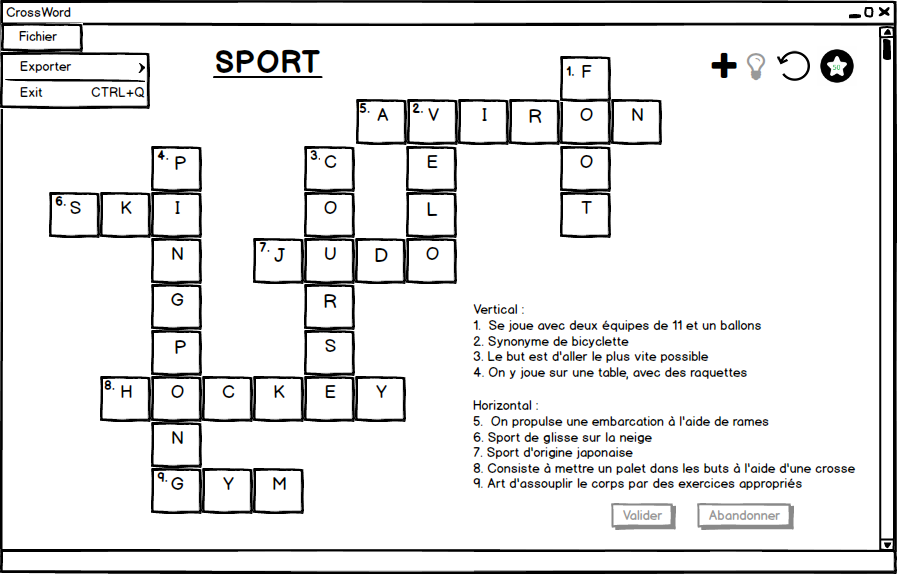
\includegraphics[height=3in]{Maquettes/Grille_solution_file.png}
        \caption{Maquette - Menu fichier} 
    \end{center}
    \end{figure}
    
   \begin{figure}[H]
    \begin{center}
        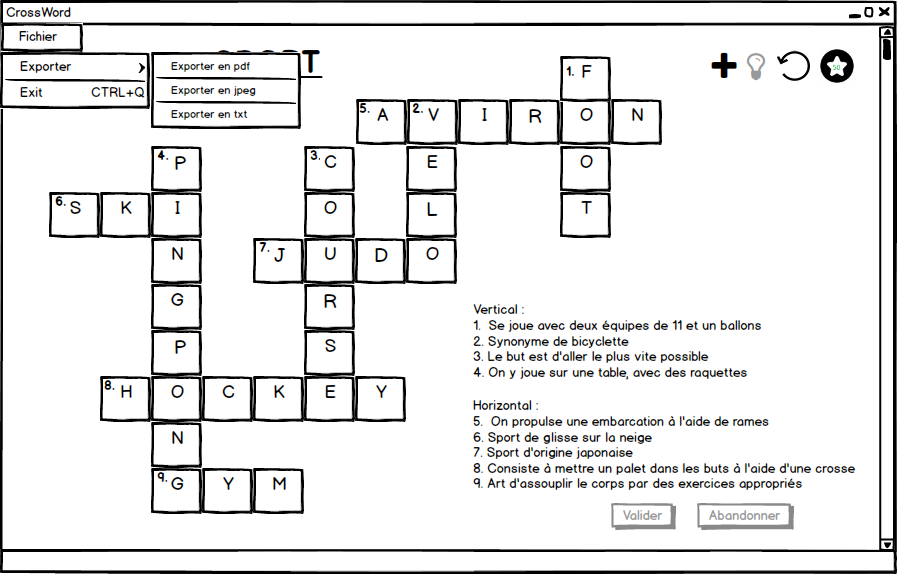
\includegraphics[height=3in]{Maquettes/Grille_solution_export.png}
        \caption{Maquette - Menu export} 
    \end{center}
    \end{figure}

\noindent{\underline{Format pdf}} : Le format pdf est mis à disposition en vue d'une impression, la grille est affichée de manière classique tel qu'elle était au moment de l'importation.\\
\underline {Format jpeg} : Le format jpeg est mis à disposition en vue d'un partage, la grille est affichée de manière classique telle qu'elle était au moment de l'importation.\\
\underline {Format txt} : Le format txt est mis à disposition en vue d'une importation future de la grille. La grille est codée (cf. "Importer une grille" pour la description du codage). \\ \\
\noindent{\underline {Test associé}} :
 \begin{tcolorbox}[colback=positifC]
            \begin{enumerate}
                \item \textit{Description et but du test} : Sauvegarde de la grille en cours avec une possibilité de choix de trois extensions differentes : .PDF, .JPG, .TXT .\newline
                
                \item \textit{Cas de test} : Avec l'utilisation d'une grille "témoin", cette dernière doit être sauvegardée sous l'extension choisie par l'utilisateur, à l'emplacement choisi par l'utilisateur grâce à l'ouverture de l'explorer. Cette grille doit pouvoir être rechargée par notre application afin que l'utilisateur puisse poursuivre sa partie. \newline
                
                \item \textit{Déroulement et scénario du test} : L'utilisateur clique sur le "Fichier" puis "Exporter" et il choisit l'extension ".TXT" parmi les trois proposées. L'explorateur de fichier s'ouvre afin que l'utilisateur puisse sélectionner son emplacement de sauvegarde. Une fois la grille sauvegardée, il devra pouvoir la recharger(cf. voir besoin "Importer une grille"). \newline
                
                \item \textit{Analyse du test} : Une comparaison de fichier entre une grille temoin sauvegardée en format .TXT par l'utilisateur à un moment defini X du jeu et une grille temoin (en guise de test Oracle) définie préalablement. Les deux fichiers comparés ne doivent montrer aucune différence.
            \end{enumerate}
        \end{tcolorbox}


\newpage
\noindent{{\color{blue}\textbf{(C) Choisir une aide}}} \\ \\ %(Systeme de vie qui change selon la difficulté)
\underline {Acteur} : Utilisateur. \\
\underline {Résumé} : L'utilisateur choisit d'être aidé pour se débloquer. \\
\underline {Préconditions} : L'application est correctement lancé (affichage du menu de selection des paramètres), une partie est commencée et la grille est correctement affichée. \\
\underline {Post conditions} : Une aide a été affichée dans la grille. \\\\
\underline {Enchaînement nominal "Réveler la case"} : 
\begin{table}[H]
\centering
\begin{tabular}{|c|c|c| c|}
\hline
\textbf{Étapes} & \textbf{Utilisateur}              & \textbf{Système}  & \textbf{Maquette correspondante} \\ \hline
1                 & \begin{tabular}[c]{@{}c@{}}Selectionne\\ une case\end{tabular} &     &/\\ \hline
2                 &                                                                & \begin{tabular}[c]{@{}c@{}}Prend en compte la case\\ sélectionnée\end{tabular}   & /     \\ \hline
3                 & \begin{tabular}[c]{@{}c@{}}Clique sur \\"Choisir une aide" \end{tabular}& {\color[HTML]{333333} }   & / \\ \hline
4 &
   &
  Affiche les différentes aides  & Maquette - Aides\\ \hline
5 &
  Choisit "Révéler la case" & &/
   \\ \hline
6 &
   & \begin{tabular}[c]{@{}c@{}}Affiche la lettre de la case\\ correspondante\end{tabular} & /\\ \hline
7 &  & \begin{tabular}[c]{@{}c@{}}Actualise les points d'aide\\ de l'utilisateur\\ (cf. explication des points d'aide)\end{tabular} &/ \\ \hline
\end{tabular}
\end{table}
\noindent{\underline {Enchaînement nominal "Réveler le mot"}} : 
\begin{table}[H]
\centering
\begin{tabular}{|c|c|c|c|}
\hline
\textbf{Étapes} &
  \textbf{Utilisateur} &
  \textbf{Système}&\textbf{Maquette correspondante} \\ \hline
1 &
  \begin{tabular}[c]{@{}c@{}}Sélectionne\\ une définition\end{tabular} & &/
   \\ \hline
2 &
   &
  \begin{tabular}[c]{@{}c@{}}Prend en compte la définition\\ sélectionnée\end{tabular} & /\\ \hline
3 &
   \begin{tabular}[c]{@{}c@{}}Clique sur\\ "Choisir une aide"\end{tabular} & & /
  {\color[HTML]{333333} } \\ \hline
4 &
   &
  Affiche les différentes aides  & Maquette - Aides\\ \hline
5 &
  Choisit "Révéler le mot" & &/
   \\ \hline
6 &
   &
  \begin{tabular}[c]{@{}c@{}}Affiche le mot correspondant \\ dans la grille\end{tabular} &/ \\ \hline
7 &  & \begin{tabular}[c]{@{}c@{}}Actualise les points d'aide\\ de l'utilisateur\\ (cf. explication des points d'aide)\end{tabular} &/\\ \hline
\end{tabular}
\end{table}
\newpage
\noindent{\underline {Enchaînement nominal "Vérifier la case"}} : 
\begin{table}[H]
\centering
\begin{tabular}{|c|c|c|c|}
\hline
\textbf{Étapes} & \textbf{Utilisateur}              & \textbf{Système} & \textbf{Maquette correspondante}\\ \hline
1                 & \begin{tabular}[c]{@{}c@{}}Sélectionne\\ une case\end{tabular} &    & /                                                                                  \\ \hline
2                 &                                                                & \begin{tabular}[c]{@{}c@{}}Prend en compte la case\\ sélectionnée\end{tabular} & /      \\ \hline
3                 & \begin{tabular}[c]{@{}c@{}}Clique sur \\"Choisir une aide" \end{tabular}                                 & {\color[HTML]{333333} }  &/                                                            \\ \hline
4                 &                                                                & Affiche les différentes aides  & Maquette - Aides                                                       \\ \hline
5                 & Choisit "Vérifier la case"                                      &     & /                                                                                 \\ \hline
6                 &                                                                & \begin{tabular}[c]{@{}c@{}}Affiche si la lettre est bonne\\ ou mauvaise\end{tabular} &/ \\ \hline
7 &  & \begin{tabular}[c]{@{}c@{}}Actualise les points d'aide\\ de l'utilisateur\\ (cf. explication des points d'aide)\end{tabular} &/ \\ \hline
\end{tabular}
\end{table}
\noindent{\underline {Enchaînement nominal "Vérifier le mot"}} : 
\begin{table}[H]
\centering
\begin{tabular}{|c|c|c|c|}
\hline
\textbf{Étapes} &
  \textbf{Utilisateur} &
  \textbf{Système} &\textbf{Maquette correspondante}\\ \hline
1 &
  \begin{tabular}[c]{@{}c@{}}Sélectionne\\ une définition\end{tabular} & &/
   \\ \hline
2 &
   &
  \begin{tabular}[c]{@{}c@{}}Prend en compte la définition\\ sélectionnée\end{tabular}&/ \\ \hline
3 &
  \begin{tabular}[c]{@{}c@{}}Clique sur\\ "Choisir une aide"\end{tabular} &&/
  {\color[HTML]{333333} } \\ \hline
4 &
   &
  Affiche les différentes aides & Maquette - Aides\\ \hline
5 &
  Choisit "Vérifier le mot" &&/
   \\ \hline
6 &
   &
  \begin{tabular}[c]{@{}c@{}}Affiche si le mot est bon\\ ou mauvais\end{tabular} &/\\ \hline
7 &  & \begin{tabular}[c]{@{}c@{}}Actualise les points d'aide\\ de l'utilisateur\\ (cf. explication des points d'aide)\end{tabular} &/\\ \hline
\end{tabular}
\end{table}

    \begin{figure}[H]
    \begin{center}
        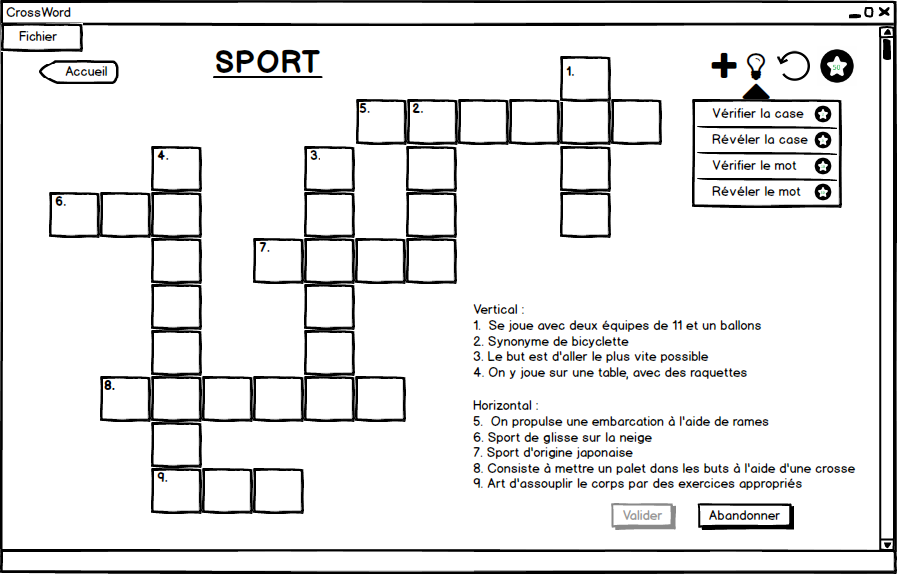
\includegraphics[height=3in]{Maquettes/Grille_aides.png}
        \caption{Maquette - Aides} 
    \end{center}
    \end{figure}

\noindent{\underline {Explication des points d'aide}} : Lors d'une partie, l'utilisateur aura tant de points (ce nombre de points sera fixé par la difficulté de la grille). A chaque utilisation d'une aide, l'utilisateur perdra des points, selon la "force" de l'aide plus ou moins de points seront enlevés : Vérifier la case $<$ Révéler la case $<$ Vérifier le mot $<$ Révéler le mot. Si l'utilisateur n'a plus de points, il ne peut plus utiliser d'aides. \\ \\
\noindent{\underline {Tests associés}} :
\begin{tcolorbox}[colback=positifC]
            \begin{enumerate}
                \item \textit{Description et but du test} : Bon fonctionnement des options d'aide.\newline
                
                \item \textit{Cas de test} : A partir d'une grille non finie, l'utilisateur doit pouvoir sélectionner les différentes aides proposées par notre programme si son nombre de point le permet.   \newline
                
                \item \textit{Déroulement et scénario du test} : L'utilisateur choisit d'utiliser l'aide "réveler le mot", "réveler la case", "vérifier la case", "vérifier le mot". \newline
                
                \item \textit{Analyse du test} : Vérifier que l'aide seléctionnée fonctionne correctement et que les points associés à l'utilisation de cette aide sont bien décomptés aux points restants à l'utilisateur.
            \end{enumerate}
        \end{tcolorbox}
        
        \begin{tcolorbox}[colback=negatifC]
            \begin{enumerate}
                \item \textit{Description et but du test} : Utilisation d'une aide avec un nombre de points insuffisant.\newline
                
                \item \textit{Cas de test} : L'utilisateur souhaite utiliser une aide mais n'a pas assez de points. Son utilisation doit être refusée  \newline
                
                \item \textit{Déroulement et scénario du test} : Cliquer sur l'utilisation d'une aide avec un nombre de points inférieur à celui demandé pour utiliser l'aide \newline
                
                \item \textit{Analyse du test} : Vérifier que l'aide n'ait pas été éxécutée.
            \end{enumerate}
        \end{tcolorbox}


\newpage
{\noindent{\color{blue}\textbf{(C) Dévoiler la grille - abandonner }}}\\ \\
\underline {Acteur} : Utilisateur. \\
\underline {Résumé} : L'utilisateur veut voir la solution complète, même s'il n'a pas commencé à remplir la grille. \\
\underline {Préconditions} : L'application est correctement lancée, la grille a été générée et affichée. \\
\underline {Post conditions} : La solution de la grille est affichée, et l'utilisateur n'aura plus la possibilité de valider. \\\\
\underline {Enchaînement nominal} : 
\begin{table}[H]
\centering
\begin{tabular}{|c|c|c|c|}
\hline
\textbf{Étapes} &
  \textbf{Utilisateur} &
  \textbf{Système} &
  \textbf{Maquette correspondante} \\ \hline
1 &
  \begin{tabular}[c]{@{}c@{}}Clique sur le bouton \\ "Abandonner"\end{tabular} &
   &
  \begin{tabular}[c]{@{}c@{}}(cf. Maquette - Grille vide, \\Bouton "Abandonner")\end{tabular} \\ \hline
2 &  & \begin{tabular}[c]{@{}c@{}}Affiche \\ la grille remplie\end{tabular} & \multirow{2}{*}{Maquette - Solution} \\ \cline{1-3}
3 &
   &
  \begin{tabular}[c]{@{}c@{}}Bloque\\  la validation de la grille\end{tabular} &
   \\ \hline
\end{tabular}
\end{table}

    \begin{figure}[H]
    \begin{center}
        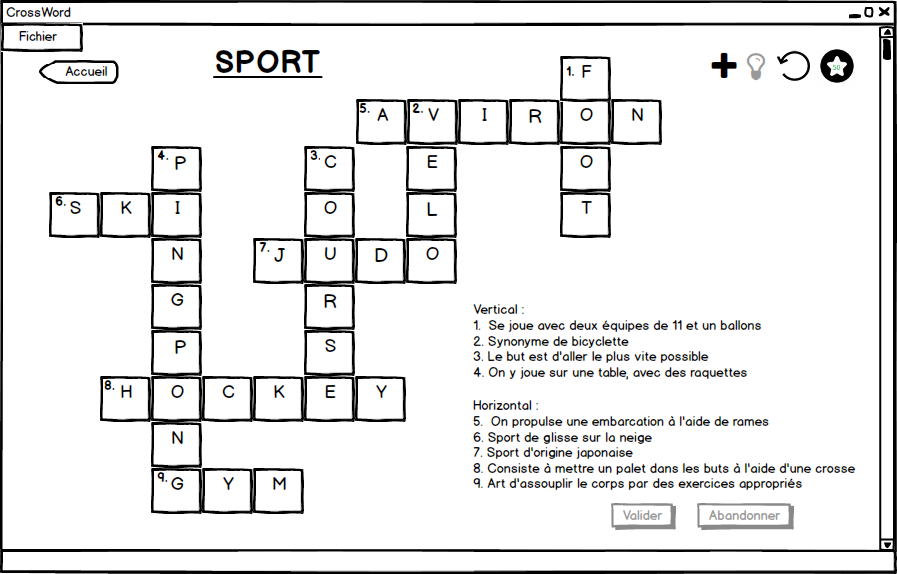
\includegraphics[height=3in]{Maquettes/Grille_solution.png}
        \caption{Maquette - Solution} 
    \end{center}
    \end{figure}

\noindent{\underline {Tests associés}} :
 \begin{tcolorbox}[colback=positifC]
            \begin{enumerate}
                \item \textit{Description et but du test} : Dévoiler toutes les cases restantes de la grille .\newline
                
                \item \textit{Cas de test} : A partir d'une grille non finie, l'utilisateur doit pouvoir dévoiler l'entièreté de la grille. Chaque case non dévoilée sera remplacée par la lettre associée.   \newline
                
                \item \textit{Déroulement et scénario du test} : L'utilisateur clique sur le bouton "Abandonner". Chaque case est remplacée par la lettre associée. \newline
                
                \item \textit{Analyse du test} : Vérifie que toutes les cases de la grille ont bien une lettre associée. Comparaison de la grille dévoilée "temoin" et une grille construite préalablement (test Oracle).
            \end{enumerate}
        \end{tcolorbox}
        
        \begin{tcolorbox}
            \begin{enumerate}
                \item \textit{Description et but du test} : Dévoiler la grille sur une grille finie.\newline
                
                \item \textit{Cas de test} : A partir d'une grille  finie et correctement completée, l'utilisateur a toujours accès au bouton "Abandonner". \newline
                
                \item \textit{Déroulement et scénario du test} : L'utilisateur a correctement completé la grille mais le bouton "Abandonner" est toujours visible. \newline
                
                \item \textit{Analyse du test} : Vérifier que le bouton "Abandonner" n'est plus disponible lorsqu'une grille est finie et correctement remplie.
            \end{enumerate}
        \end{tcolorbox}

\newpage
\noindent{{\color{blue}\textbf{(E) Valider la grille}}} \\ \\
\underline {Acteur} : Utilisateur. \\
\underline {Résumé} : L'utilisateur valide sa solution après avoir rempli la grille en entier. Il saura alors combien de mots il a correctement deviné et le nombre d'erreurs effectuées. \\
\underline {Préconditions} : L'application est correctement lancée, la grille a été générée, affichée et l'utilisateur l'a remplie. \\
\underline {Post conditions}: L'utilisateur a fini, les mots correctement devinés et le nombre d'erreurs sont affichés. \\\\
\underline {Enchaînement nominal} : 
\begin{table}[H]
\centering
\begin{tabular}{|c|c|c|c|}
\hline
\textbf{Étapes} &
  \textbf{Utilisateur} &
  \textbf{Système} &
  \textbf{Maquette correspondante} \\ \hline
1 &
  \begin{tabular}[c]{@{}c@{}}Clique sur le bouton \\ "Valider" \end{tabular} & & Maquette - Grille remplie \\ \hline
2 &  & \begin{tabular}[c]{@{}c@{}}Affiche les mots \\ correctement devinés\end{tabular} & \multirow{3}{*}{Maquette - Validation} \\ \cline{1-3}
3 &
   &
  \begin{tabular}[c]{@{}c@{}}Affiche \\ le nombre d'erreurs\end{tabular} &
   \\ \cline{1-3}
4 &
   &
  \begin{tabular}[c]{@{}c@{}}Met à jour\\  le score\end{tabular} &
   \\ \hline
\end{tabular}
\end{table}

    \begin{figure}[H]
    \begin{center}
        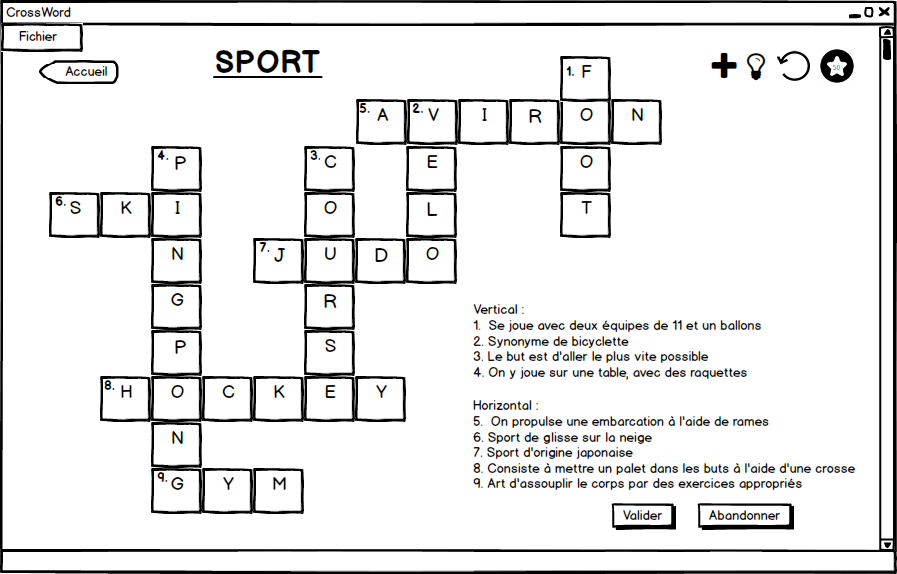
\includegraphics[height=3in]{Maquettes/Grille_remplie.png}
        \caption{Maquette - Grille remplie} 
    \end{center}
    \end{figure}
    
      \begin{figure}[H]
    \begin{center}
        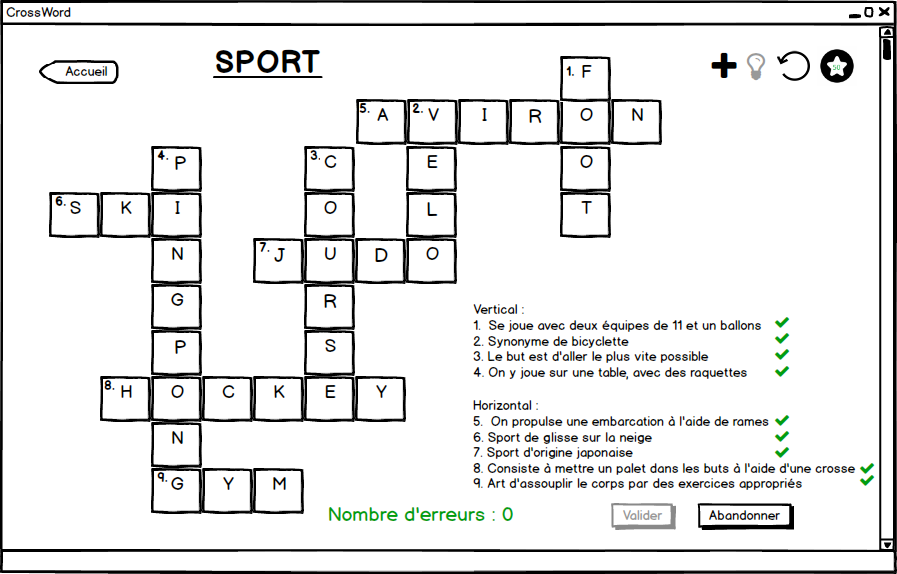
\includegraphics[height=3in]{Maquettes/Grille_validation.png}
        \caption{Maquette - Validation} 
    \end{center}
    \end{figure}

\subsection{Besoins système}
Le besoin système principal concerne la génération de la grille. Nous devons être sûrs que la grille affichée à l'utilisateur a une solution. Pour cela nous devons donc coder un solver de grille qui trouvera la solution pour une grille donnée (si elle existe). Grâce à ce solver nous pourrons stocker la solution de la grille ce qui permettra également à l'utilisateur de jouer en vérifiant ses réponses et en utilisant les aides. Pour cela nous allons représenter la génération de grille de mots croisés comme un problème de satifaction de contraintes.  
L'encodage sous forme de CSP est décrit en section "6.2 VARIABLE - Champ accueillant un mot".
L'algorithme du solver est quant à lui décrit plus loin en section "6.4 Algorithme d'attribution des mots aux Variables - Solver".

\newpage
\section{Besoins non fonctionnels}
\subsection{Besoins d’utilisabilité}
\noindent{{\color{blue}\textbf{(E) Interface graphique}}} \\
Notre grille de mots croisés sera jouable sur une simple interface graphique, disposant de la grille et d'un menu. Cette interface devra être simple d'utilisation. \\

\noindent{{\color{blue}\textbf{(E) Manuel d'utilisation}}} \\
Notre programme disposera d'un court manuel d'utilisation afin de préciser les différents points sur l'utilisation de notre grille de mots croisés et sur l'utilisation des différents menus de notre application. \\

\noindent{{\color{blue}\textbf{(E) Langue du programme}}} \\
Tout le programme (interface, mots de la grille et menu) devra être écrit en Anglais.

\subsection{Besoins de performances}
\noindent{{\color{blue}\textbf{(E) Temps de génération de la grille de mots croisés}}} \\
Toute génération de grille de mots croisés (quelque soit les paramètres choisis par l'utilisateur) doit se faire dans l'ordre de la seconde. Notons que cela concerne \textbf{uniquement} les grilles disponibles à l'utilisateur. 
Une attention particulière sur la complexité de l'algorithme de génrération ainsi que sur les tests de génération de la grille devra être apportée.

\subsection{Besoins de sécurité}
\noindent{{\color{blue}\textbf{(E) Sécurité}}} \\
L'utilisation de notre programme ne requiert aucune connexion internet (sauf pour l'installation des librairies nécéssaires à l'interface graphique), de ce fait aucune donnée personnelle propre à l'utilisateur ne sera sauvegardée ou utilisée ultérieurement.

\pagebreak
\newpage


\section{Parallèle entre notre analyse initiale et les choix faits lors du développement}

    L'analyse des besoins présentée plus haut a été réalisée au début du projet avant de commencer son implémentation. Nous allons maintenant présenter et argumenter les différences entre cette première analyse et les choix qui ont été effectivement mis en place lors du développement.\\

    \subsection{Maquettes}
        Dans un premier temps nous nous sommes rendu compte que les grilles de mots croisés sont des grilles carrées ou rectangles contenant des cases noires et ne sont pas seulement composées des mots qui s'intersectent.  Voici une mise à jour de l'interface actuelle :
    
        \begin{figure}[H]
        \begin{center}
        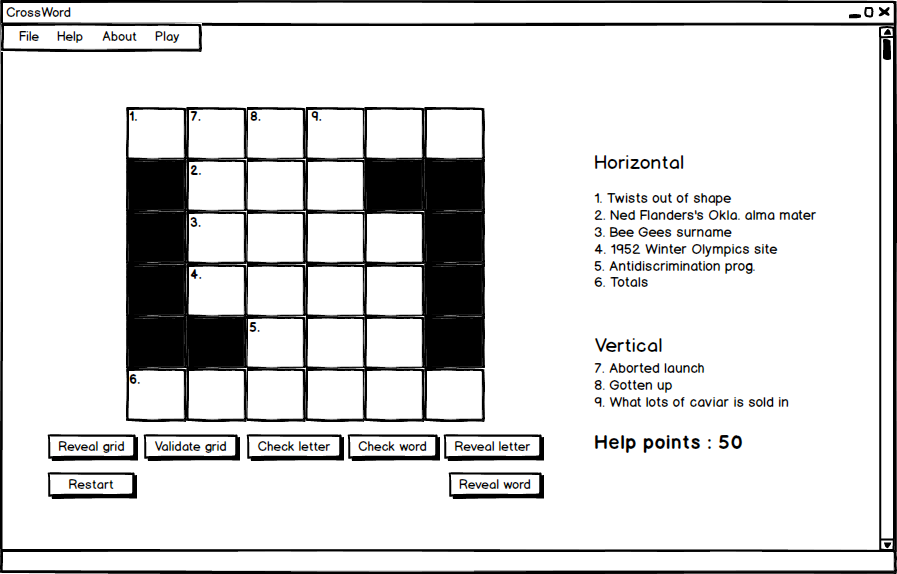
\includegraphics[height=3in]{Maquettes/finales/Grille_vide.png}
        \caption{Maquette finale - Grille vide} 
        \end{center}
        \end{figure}
        
        \begin{figure}[H]
        \begin{center}
        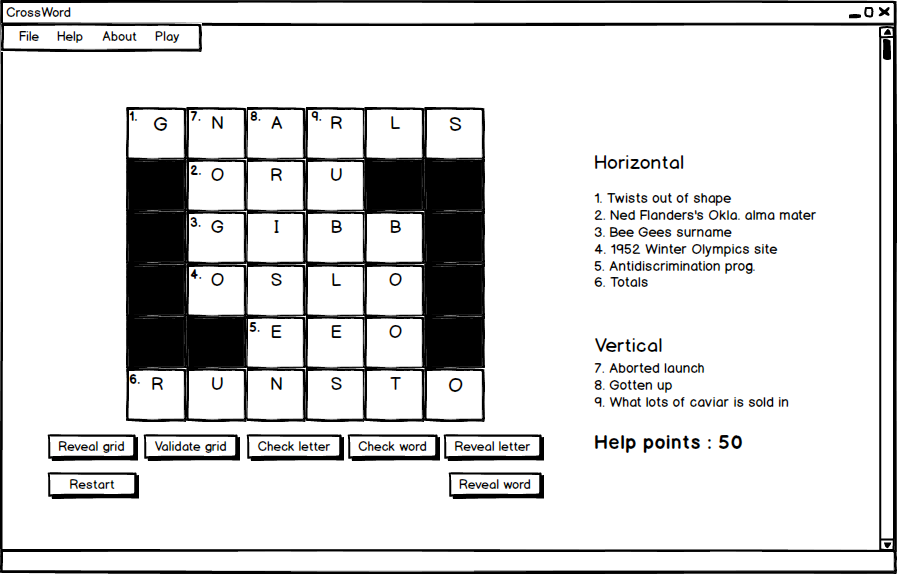
\includegraphics[height=3in]{Maquettes/finales/Grille_remplie.png}
        \caption{Maquette finale - Grille remplie} 
        \end{center}
        \end{figure}
    \subsection{Patterns}
        Nous avons aussi fait le choix d'appliquer notre algorithme sur des grilles ayant des cases noires déjà placées. Pour cela nous avons créé une dizaine de motifs de grille pour chaque niveau de difficulté (facile, normal, difficile). Lors de la génération, nous choisirons une grille du bon niveau de difficulté et nous lui appliquerons notre solver (cf. "6.5 Algorithme d'attribution des mots aux Variables - Solver") afin d'être sûrs que la grille ait une solution. Ce choix des cases noires déjà placées au lieu d'un algorithme qui les placerait au fur et à mesure sur la grille vide s'il ne trouve pas de mots nous a permis d'éviter d'avoir à effectuer un parcours sur une liste de champs qui change constamment. 
        
        \begin{figure}[H]
            \begin{center}
            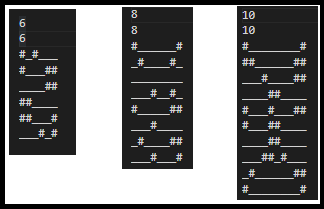
\includegraphics[height=2in]{patterns.png}
            \caption{Exemple de patterns pour chaque difficulté} 
            \end{center}
            \end{figure}
    
    \subsection{Format de données pour l'importation et l'exportation}
        Lors de notre conception nous pensions que nous allions créer nos fichiers d'importations et d'exportations avec des fichiers au format \textit{txt}. Or, lors du développement de ces fonctionnalités, nous avons remarqué que manipuler ces fichiers \textit{txt} devenait fastidieux (problème encodage entre différentes architectures). Nous avons donc réfléchi à une alternative et nous avons choisi le format de données \textit{JSON}.
        \\\\
        Le fichier d'importation regroupe l'état du jeu :
        \begin{itemize}
            \item la difficulté
            \item le nombre de points d'aides restants
            \item la grille du joueur
            \item la solution générée par notre algorithme
            \item les définitions/indices associés aux mots de la grille
        \end{itemize}
        
        \begin{figure}[H]
            \begin{center}
            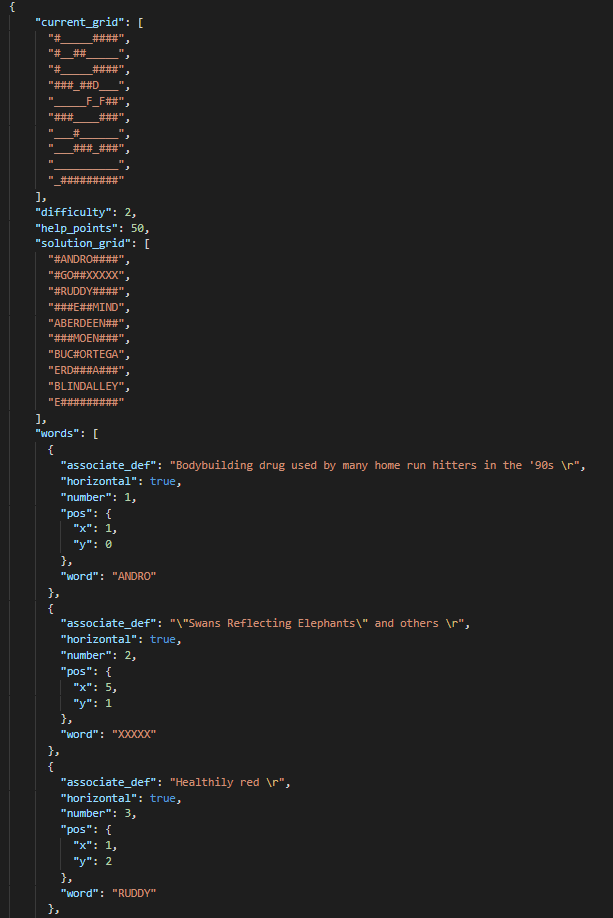
\includegraphics[height=1\linewidth]{import_file.png}
            \caption{Exemple de fichier d'importation} 
            \end{center}
            \end{figure}

\newpage
\section{Représentation du jeu des mots croisés et algorithmes}
    \subsection{SOLVER - Coeur de l'algorithme de génération}

    Le \textit{solver} contient tous les éléments nécessaires à la résolution d'une grille. Plus précisément il contient les élements suivants:

    \begin{itemize}
        \item un \textit{pattern} : configuration initiale de la grille, seule la position des cases noires et les dimensions de la grille y sont présentes.
        \item une liste des \textit{variables} de la grille (cf. section "VARIABLE - Champ accueillant un mot"). 
        \item le nombre de ces variable.
        \item les mots qui ont déjà été placés
        \item la grille sur laquelle on travaille
    \end{itemize}
    
    L'ensemble des variables sera initalisé grâce à notre \textbf{Algorithme d'initialisation des Variables} (cf section 6.3).
        
    Ensuite, la résolution se fera en suivant l'\textbf{Algorithme d'attribution de mots aux Variables} (cf section 6.4).
    
    \subsection{VARIABLE - Champ accueillant un mot}
    
    Afin de représenter le problème de la génération des mots croisés sous format de \textbf{CSP} (problème de satisfaction de contraintes), il convient de définir plus précisément ici les \textit{variables}.
    
    Pour cela, chaque variable contiendra les élements suivants : 
    \begin{itemize}
        \item le mot qu'elle contient et sa taille (à l'initialisation ce mot est défini à \textit{null}).
        \item les autres variables avec lesquelles elles s'intersectent (ainsi que les positions d'intersection).
        \item sa position absolue dans la grille.
        \item un booléen pour savoir si le mot stocké est vertical ou horizontal.
        \item le \textit{domaine} :  ensemble des mots possibles pour une variable (en tenant compte des contraintes) ainsi que sa cardinalité.
    \end{itemize}
    
    Pour une variable les contraintes sont : la taille du mot que l'on doit trouver ainsi que des lettres précises qui doivent se trouver à certaines positions en fonction des mots qui ont déjà été placés. \\\\
    Le \textit{domaine} est un sous ensemble du \textbf{lexique, i.e la base de données (Cf Section 6.5)}. Initialement il contient tous les mots du \textit{lexique} d'une longueur égale à l'espace occupé par la \textit{variable}. Par la suite il sera régulièrement mis à jour afin d'enlever les mots qui ne respectent plus les contraintes.
        
        

    \subsection{Algorithme d'initialisation des Variables}
    Cet algorithme permet d'initialiser le tableau de variable de la grid en prenant en entrée cette même grille initialisée à partir d'un pattern de grille. En sortie, chacune des variables du tableau sera initialisée et disposera de :
    \begin{itemize}
        \item son mot (initialisé à \textit{null})
        \item son \textit{domaine} 
        \item sa taille
        \item son orientation
        \item sa position (case où débutera le mot)
        \item ses voisins (autres variables qui ont des cases en commun)
    \end{itemize}
    
    %Entrées: fichier pattern
    %Sorties: tableau de variables de grid initialisé
    \begin{algorithm}[H]
    \caption{Algorithme d'initialisation des Variables}\label{alg:cap}
    \begin{algorithmic}
    \State case\_precedente $\gets$ case\_noire
    \State case\_actuelle $\gets$ case\_noire
    \State taille\_mot $\gets$ 0 \\
    \For{Chaque colonne {i}}
        \For{Chaque ligne {j}}
            \State case\_precedente $\gets$ case\_actuelle
            \State case\_actuelle $\gets$ case[i][j]
            \If{(case\_precedente = case\_noire ET case\_actuelle = case\_blanche)}
                \State taille\_mot $\gets$ taille\_mot + 1
                \State Retient la position
            \EndIf
            \If{(case\_precedente = case\_blanche ET case\_actuelle = case\_blanche)} 
                \State taille\_mot $\gets$ taille\_mot + 1
            \EndIf
            \If{(case\_precedente = case\_blanche ET case\_actuelle = case\_noire)}
                \If{(taille\_mot $\ge$ 3{\color{red}*})}
                    \State Créer variable (avec  position, direction horizontale et taille\_mot)
                \EndIf
            \EndIf
        \EndFor
        \If{(case\_actuelle = case\_blanche ET (taille\_mot $\ge$ 3{\color{red}*}))} 
                \State Créer variable (avec  position, direction horizontale et taille\_mot)
        \EndIf
        \State taille\_mot $\gets$ 0   
        \State case\_actuelle $\gets$ case\_noire    
    \EndFor \\
    \For{Chaque ligne {i}}
        \For{Chaque colonne {j}}
        \State De la même façon, créer les variables verticales
        \EndFor
    \EndFor \\
    
    \For{Chaque variable {v}}
        \State Initialiser le domaine de v 
        \For{Chacun de ses voisins {w}}
            \State Définir w comme voisin de v 
        \EndFor
    \EndFor
    \end{algorithmic}
    \end{algorithm}
    
    \noindent{{\color{red}*} Plus petit mot possible que nous avons décidé d'utiliser.}
    Pour simplifier la lisibilité de l'algorithme le calcul de la position a volontairement été omis. 
    
        \newpage

    \subsection{Algorithme d'attribution des mots aux Variables (Solver) }
    
    Pour générer une grille qui a une solution, l'objectif est d'associer un mot à chaque \textit{variable} tout en respectant les contraintes de celle-ci.

    \begin{algorithm}[H]
    \caption{Algorithme d'attribution des mots aux Variables}\label{alg:cap}
    \begin{algorithmic}
    \While{Toutes les variables ne sont pas assignées}
    \State Calculer la taille du domaine de chaque Variable de la grille
    \State Variable v = variable dont la cardinalité associée au domaine est minimale
    \State word = premier mot du domaine de v
        \If{(word != NULL)}
            \State Valeur de v $\gets$ word
            \State Mettre à jour les domaines des voisins de v
           \Else 
                \State On retourne en arrière et on teste la valeur suivante pour la variable précédente
        \EndIf
    \EndWhile
    \end{algorithmic}
    \end{algorithm}
    
    Par un processus de randomisation du \textit{domaine} des \textit{variable}s, deux appels sur une même \textit{grid} pourront produire plusieurs grilles différentes.
    
    Si une solution à la grille peut-être trouvée, alors elle sera proposée à l'utilisateur avec les définitions associées et les mots non révélés.
    
    %\subsection{PATTERN - Structure d'une grille}
    %Les motifs sont créés de manières à avoir seulement des champs pouvant contenir des mots de taille 3 ou plus car les mots de notre base de données sont de taille 3 minimum.

    \subsection{Lexique (base de données) - Stockage des mots}
    
    Notre solver (décrit via l'algorithme 2) nécessite une base de données de mots. Nous allons présenter ici son implémentation abstraite. 
    Nous allons pour cela utiliser des tableaux de bits pour stocker nos mots. C'est en effet sous cette représentation que l'on trouve les meilleures performances en terme de recherche algorithmiques de mots selon des critères précis d'après \cite{Cpc}. Par exemple, ce stockage permet de trouver un mot de longueur 5 dont la première lettre est un \textit{a} et la 3ème un \textit{c} en \textbf{O($d/32$)} avec \textbf{d} les valeurs que peuvent prendre chacune des variables (énoncé en section précédente). \\
    
    Ainsi, cela permet de trouver un mot avec une complexité \textbf{linéaire}. De plus, la représentation de cette base de données de mots sous forme de tableaux de bits permet de minimiser l'espace mémoire utilisé. En effet, pour un dictionnaire de \textbf{20 000} mots, seuls 2.4 Mb d'espace seront utilisés. Concentrons nous maintenant sur l'implémentation de ce tableau de bits. Pour simplifier, nous allons donner un exemple de la gestion globale des mots dans notre base de données :
    
    \begin{figure}[H] 
    \center 
    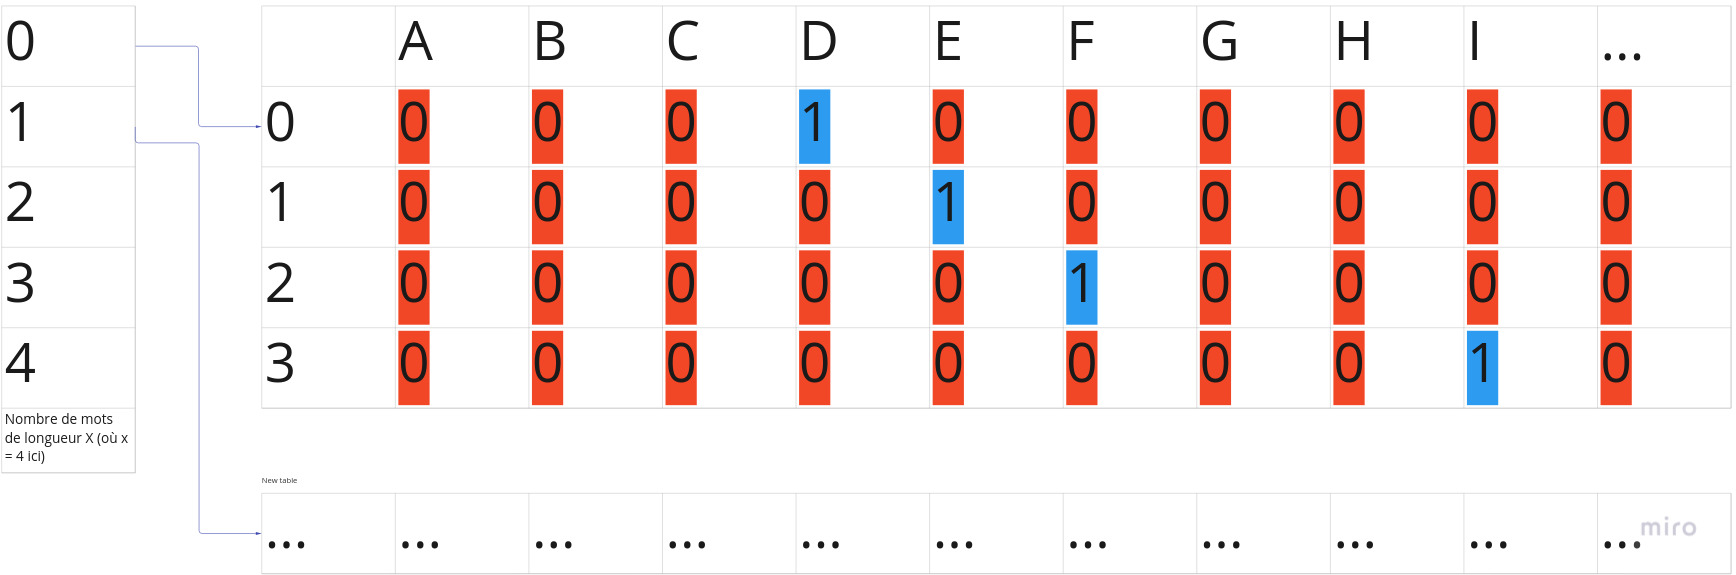
\includegraphics[width=1\linewidth]{database_schema.jpg}
    \end{figure}
    
    Sur la figure ci-présente, nous présentons comment le mot "\textbf{defi}" est stocké. Ici, le tableau en vert représente le tableau où chaque indice correspond à des mots de longueurs 4. Il y a ainsi un tableau de pointeurs (menant à des tableaux 2D pour chaque mot) par longueur de mot. Ce stockage nous permet de trouver très rapidement un mot de telle longueur possédant telle lettre à tel indice, et donc de l'intersecter éventuellement aussi avec un autre mot possédant d'autre caractéristiques dans le but de construire la grille.
    \\\\On aura donc :
    \begin{itemize}
        \item Pour chaque longueur de mot de taille X, un tableau d'entier de longueur \textit{nbMotTailleX}.
        \item Pour chaque mot un tableau de taille \textit{nbLettre}
        \item Pour chaque lettre un tableau de bits de taille 26
    \end{itemize}
    
    Cela se fait grâce à notre \textbf{Algorithme d'encodage des mots en tableau de bits} :
    

    \subsubsection{Algorithme d'encodage des mots en tableau de bits}
    
    Ci-après l'algorithme que nous utiliserons pour encoder notre base de données de mots en tableau de bits :
        
    \begin{algorithm}[H]
    \caption{Encodage base de donnée du lexique}\label{alg:cap}
    
    \begin{algorithmic} 
    \State $listDeMots\gets charge mot depuis notre lexique$
    \State $dBWordLength2 \gets allocation[nbTotalWord2][2][26]$ \Comment{création des tableaux pour chacune des longueurs de mot}
    
    \For{mot dans {listDeMots }} 
        ajouterMot(dbWordLenght(lenghtMot))
    \EndFor
    
    \end{algorithmic}
    \end{algorithm}
    
    Nous considérons que cet algorithme est utilisé dans notre constructeur de l'objet "DataBase" et que les dBWordLength sont ses attributs. Nous allons maintenant voir comment ajouter un mot dans un sous-tableau (fonction que nous avons appelée dans la fonction précédente) : 
    
    \begin{algorithm}
    \caption{Ajouter Mot}\label{alg:cap}
    
    \begin{algorithmic} 
    
    \For{lettre dans mot} 
        \State $index \gets lettre -'a'$
        \State $dbWord[currentWordIndex][currentWordSize][index] \gets 1 $
    \EndFor
    
    \end{algorithmic}
    \end{algorithm}
    

\newpage

\section{Techniques utilisées}

    \subsection{Langages}
    D'après l'article de thèse \cite{Cpc} qui préconise d'utiliser un tableau de bits pour la manipulation (et le stockage) de la base de données de nos mots et définitions associées; il est conseillé d'utiliser le langage \textbf{Cpp} qui permet une manipulation simple de ces derniers. Le language C est également conseillé, mais nous avons néammoins choisi le langage \textbf{Cpp} car c'est un langage objet, il nous permet un plus grand contrôle sur la structure du code et facilite l'utilisation des Designs Patterns.%lien à faire vers la section en question
    \subsection{JSON}
    On peut aussi noter l'utilisation du JSON comme format de données pour nos fichiers d'importation et d'exportation. Pour manipuler ce format de données avec du \textbf{Cpp} nous avons utilisé la library \textbf{\textit{nlohmann$\_$json}} \cite{NJs}
    \subsection{Interface Graphique}
    Il ressort de nos recherches sur les meilleures interfaces graphiques en Cpp que le framework Qt \cite{QtD} semble être le plus performant, documenté et simple d'utilisation. C'est celui que nous allons utiliser. De plus, certains du groupe l'avaient déjà utilisé, bien entendu ce paramètre est rentré en compte. 
    
    \subsection{Choix du dictionnaire}
    Comme stipulé dans les articles mentionnés dans le cahier des besoins, afin d'obtenir de bonnes performances (et obtenir une complexité de recherche / intersection de domaines \textbf{linéaire}) nous avons recherché une base de données contenant des mots issus de mots croisés, et classés par pertinence. Nous l'avons trouvée sur ce site web \cite{Bd} . En utilisant la bibliothèque \textbf{numpy} (et \textbf{pandas}) de python, nous lui avons ensuite appliqué un traitement afin de la trier par taille et récursivement par ordre alphabétique. Initialement, la base de données contenait 6 millions de mots. Nous avons jugé cela trop important (rapellons que l'article \cite{CpC} préconisait une taille d'environ 20 000 mots pour des performances optimales). Ainsi, nous avons obtenu via nos traitements une base de données de \textbf{31316} mots. Ce résultat a été obtenu en enlevant tous les mots doublons et en gardant ceux les plus pertinents (nous gardons les mots qui apparaissent au moins 25 fois). Bien entendu, chacun des mots est associé à une définition. \\
    
    Pour trier et ne garder que ces 31316 mots, notre script python est le suivant : 
    
    \begin{minted}
        [
        frame=lines,
        framesep=2mm,
        baselinestretch=1.2,
        bgcolor=LightGray,
        fontsize=\footnotesize,
        linenos
        ]
        {python}
        
import pandas
import numpy
import json


df = pandas.read_csv("xd/clues.tsv", sep='\t') #le fichier de base
df.pop("pubid") #on enlève les colonnes qui ne nous intéressent pas
df.pop("year") 
rep=df["answer"].value_counts()
common=rep[rep>=25] #on garde seulement les mots les plus communs (qui apparaissent + de 25 fois)
l=sorted(common.keys())
l=sorted(l,key=len)
with open('jsonrep/result.txt', 'w') as f:
    f.write('\n'.join(l)) #puis on écrit les mots qui nous intéressent dans notre fichier
        
    \end{minted}
    
    
    Afin de récupérer et d'encoder le fichier "mot - définition" de manière adéquate à notre application, nous avons écrits le script python suivant : 
    
    \begin{minted}
        [
        frame=lines,
        framesep=2mm,
        baselinestretch=1.2,
        bgcolor=LightGray,
        fontsize=\footnotesize,
        linenos
        ]
        {python}
        
    #!/usr/bin/python
fichierMot = open("data/word_database.txt") #mot de notre base 
FichierDef = open("data/clues.tsv") #les définitions
fichierOut = open("data/word_with_def.txt", "a") #le fichier à produire 

lignesWords = fichierMot.readlines()
lignesClues = FichierDef.readlines()

for mot in lignesWords: #parcours chacun des mots du fichier mot
    fichierOut.write(mot) #on l'écrit dans le fichier de sortie
    for clues in lignesClues: #parcourt tous les indices
      words = clues.split()
      try:
        if(words[2] + "\n" == mot):
          for i in range(3,len(words)):
            fichierOut.write(words[i] + " ")
          fichierOut.write("\n \n")
          break
      except IndexError:
          a = 5 #ne fait rien ...


fichierMot.close()
FichierDef.close()
fichierOut.close()
        
    \end{minted}
    
\newpage    

\section{Architecture de l’application}

Il a fallu réfléchir à une architecture qui nous permette de répondre à tous les besoins décrits plus haut et qui puisse accueillir notre générateur de grille.

\subsection{Démarche}
    Notre démarche a été de penser à un découpage de classes qui respecte les bonnes pratiques inculquées en génie logiciel. Chacune de nos classes ont un rôle précis, nous avons notamment voulu que tout ce qui concerne le générateur d’une grille (les algorithmes décrits dans la section "6 Représentation du jeu des mots croisés et algorithmes") ne soit pas dépendant du jeu.\\ 
    L’avantage à en tirer, au-delà des bonnes pratiques, est de permettre, dans un premier temps, de programmer le générateur de grille jusqu’à le rendre fonctionnel sans avoir à se soucier du jeu. Et une fois le générateur entièrement fonctionnel le jeu aura juste à l’utiliser pour récupérer des grilles.
    \\\\
    Un point assez important pour être à l’aise avec l’architecture est de comprendre ce qu'est l’état de notre jeu de mots croisés, cet état est contenu dans la classe \textbf{Crossword}:
    \begin{figure}[H] 
    \center 
    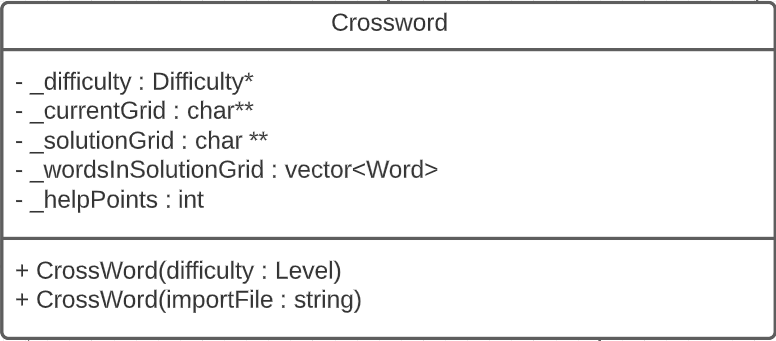
\includegraphics[width=0.5\linewidth]{crossword_uml.png}
    \caption{Classe "Crossword"}
    \end{figure}
    Nous y retrouvons:
    \begin{itemize}
        \item la difficulté des mots croisés
        \item la grille courante : la grille sur laquelle le joueur joue
        \item la grille de solution : c’est la grille remplie qui a été générée par notre générateur de grille
        \item la liste de mots de la grille : cette liste contient toutes les informations associées à chaque mot de la grille (comme par exemple leur numéro et leur définition associée)
        \item le nombre de points d’aide disponibles pour le joueur
    \end{itemize}
    
    Le jeu de mots croisés peut être construit à partir d’une difficulté : dans ce cas là on sélectionnera un pattern (lié à la difficulté choisie) au hasard et le générateur de grille générera une grille en se reposant sur le pattern sélectionné.
    \begin{figure}[H] 
    \center 
    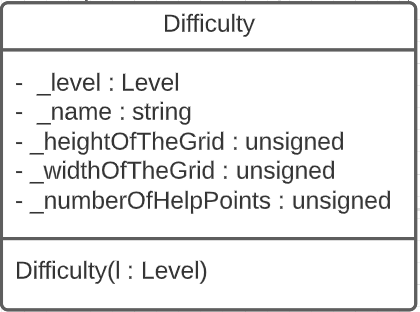
\includegraphics[width=0.3\linewidth]{difficulty_uml.png}
    \caption{Classe "Difficulty"}
    \end{figure}
    Lors de la construction du jeu, il récupère toutes les données liées à la difficulté à l’aide de la classe \textbf{Difficulty}. Cette classe est construite à partir d’un "niveau" (EASY, NORMAL, HARD) et stocke toutes les données correspondantes à cette difficulté:
    \begin{itemize}
        \item le niveau (EASY, NORMAL ou HARD)
        \item le nom littéral de la difficulté (\guillemotleft easy\guillemotright, \guillemotleft normal\guillemotright, \guillemotleft hard\guillemotright)
        \item la longueur de la grille associée à cette difficulté
        \item la largeur de la grille associée à cette difficulté
        \item le nombre de point d’aides de départ associé à cette difficulté
    \end{itemize}
    Le jeu de mots croisés peut aussi être construit à partir d’un fichier d’importation, dans ce cas là l’état stocké dans le fichier d’importation est totalement rétabli.
    \\\\
    Toutes les méthodes pour manipuler l’état du jeu de mots croisés sont réunies dans une interface, dont nous allons parler dans la section "8.3 Design patterns".
    \\\\
    Pour y voir plus clair par la suite, voici le diagramme de classes UML \textbf{\textit{simplifié}} de notre application :
    \begin{figure}[H] 
    \center 
    \includegraphics[width=0.8\linewidth]{diag_classes_simplifié.jpeg}
    \caption{Diagramme de classes simplifié}
    \end{figure}
    
    En bas à droite du diagramme ci-dessus, on peut y voir la classe \textbf{Solver} : cette classe représente notre générateur de grille de mots croisés. Nous remarquons, comme il a été expliqué plus haut, que le jeu (\textbf{Crossword}) utilise le générateur mais que lui n’est pas dépendant du jeu.\\
    Les classes \textit{Variable, Domain, Lexicon, Pattern, AttributedWords}, dont le générateur dépend rappellent tous les éléments nécessaires à la génération d’une grille, décrits dans la section "6 Représentation du jeu des mots croisés et algorithmes".
    \\\\
    Autre point concernant le découpage de nos classes : notre application possède une interface utilisateur, nous avons donc fait le choix d’utiliser le modèle \textbf{MVC} (\textit{Model-View-Controller}), pour que ni le jeu ni l’interface ne soit dépendant l’un de l’autre.
    
\subsection{Model-View-Controller}
    \begin{figure}[H] 
    \center 
    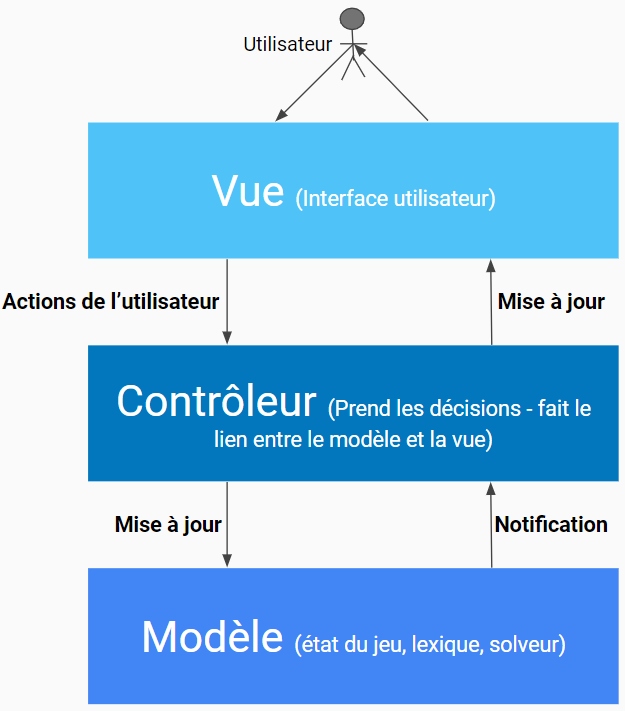
\includegraphics[width=0.4\linewidth]{mvc.png}
    \caption{Schéma de notre implémentation du MVC}
    \end{figure}
    Dans notre application, l’utilisateur interagit essentiellement avec la vue. La vue dans notre architecture correspond à la classe \textbf{MainWindow} et ses agrégations : \textbf{ShowGrid} a pour rôle d’afficher la grille de jeu du joueur, \textbf{ShowNumber} d’afficher les numéros des mots dans la grille, \textbf{DefTable} d’afficher le tableau des définitions qui sont associées aux mots de la grille. \textbf{MainWindow} les instancie quand une grille à été générée.
    \\\\
    \textbf{MainWindow} regroupe des déclencheurs qui communiquent au contrôleur chaque action de l’utilisateur. Ensuite le contrôleur, ici \textbf{CrosswordController}, manipule l’état de jeu (\textbf{Crossword}) puis communique à la vue le nouvel état à afficher.
    
\subsection{Design patterns}
    Quand la solution s’y prêtait nous avons souhaité utiliser un design pattern.  Le contrôleur du modèle MVC est d’ailleurs un design pattern, il joue le rôle de \textbf{\textit{médiateur}}.
    \\\\
    Le contrôleur utilise l’interface \textbf{CrosswordFacade} pour manipuler le jeu, cette classe est aussi un design pattern : \textbf{\textit{facade}}, il nous a permis en amont de réunir dans une interface toutes les fonctionnalités dont l’extérieur aurait besoin pour manipuler le jeu. L’implémentation de cette classe a été réfléchie avant de fabriquer l’état du jeu, ce qui nous as donné comme premier avantage d’avoir les idées claires sur toutes les fonctionnalités à implémenter dans la classe \textbf{Crossword}. Le second avantage a été de pouvoir avancer sur le développement du contrôleur (et par conséquence de la vue aussi) sans se soucier de l’avancée du développement de la classe \textbf{Crossword}.
    \\\\
    Nous pouvons aussi parlé de la classe \textbf{Lexicon} qui, elle, est un \textbf{\textit{singleton}}. En effet, nous avons besoin d’accéder au lexique tout au long de la génération. De plus, le lexique est unique nous voulons nous assurer qu’une seule instance sera créée. Le pattern \textbf{\textit{singleton}} nous a donc permis de fournir au générateur un point d’accès et aussi de nous assurer qu’il y a une unique instance du lexique.

\subsection{Diagramme de classes UML détaillé}
    Si vous ressentez le besoin de voir l’architecture de l’application de manière détaillée voici le diagramme de classes UML avec les méthodes et attributs de chaque classe. Les seules méthodes qui n’y apparaissent pas sont les getters/setters et certaines méthodes qui appartiennent au framework Qt :
    \newpage
    \begin{landscape}
        \begin{figure}[H] 
        \center 
        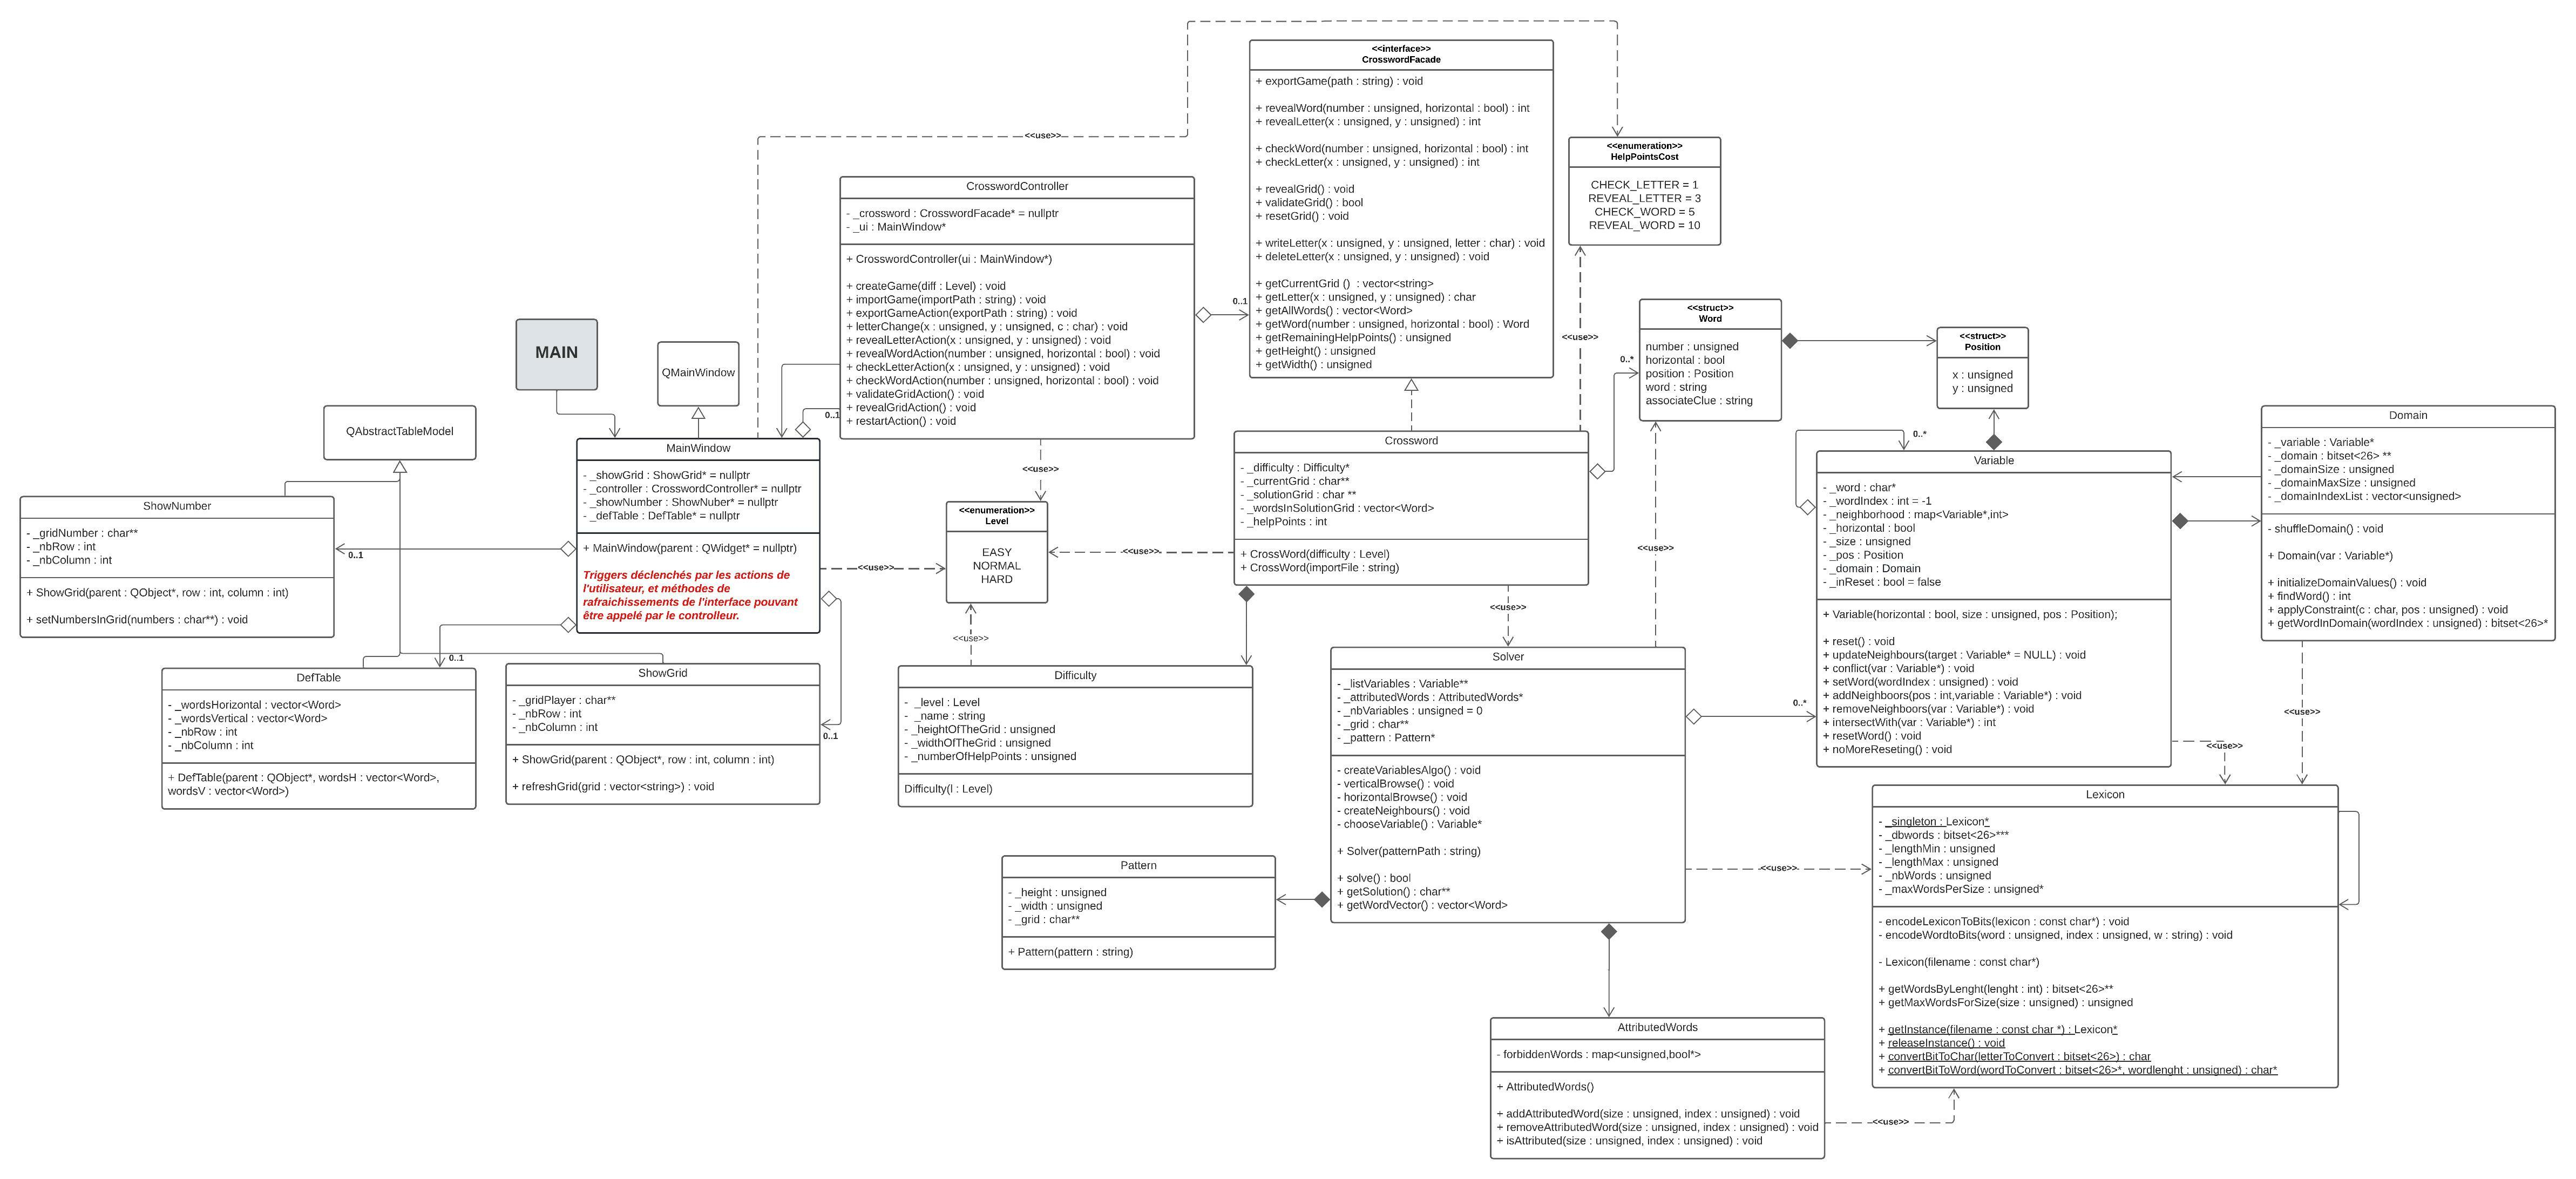
\includegraphics[width=1\linewidth]{diag_classes_complet.jpeg}
        \caption{Diagramme de classes UML détaillé de notre application}
        \end{figure}
    \end{landscape}
    \newpage
    
\subsection{Diagramme de paquetages UML}
    Un autre point intéressant de notre architecture est la répartition des classes dans les différents paquetages, en effet il y a beaucoup de classes donc une bonne répartition nous a semblé nécessaire.
    \\\\
    Voici le diagramme de paquetages UML de notre application : 
    \begin{figure}[H] 
    \center 
    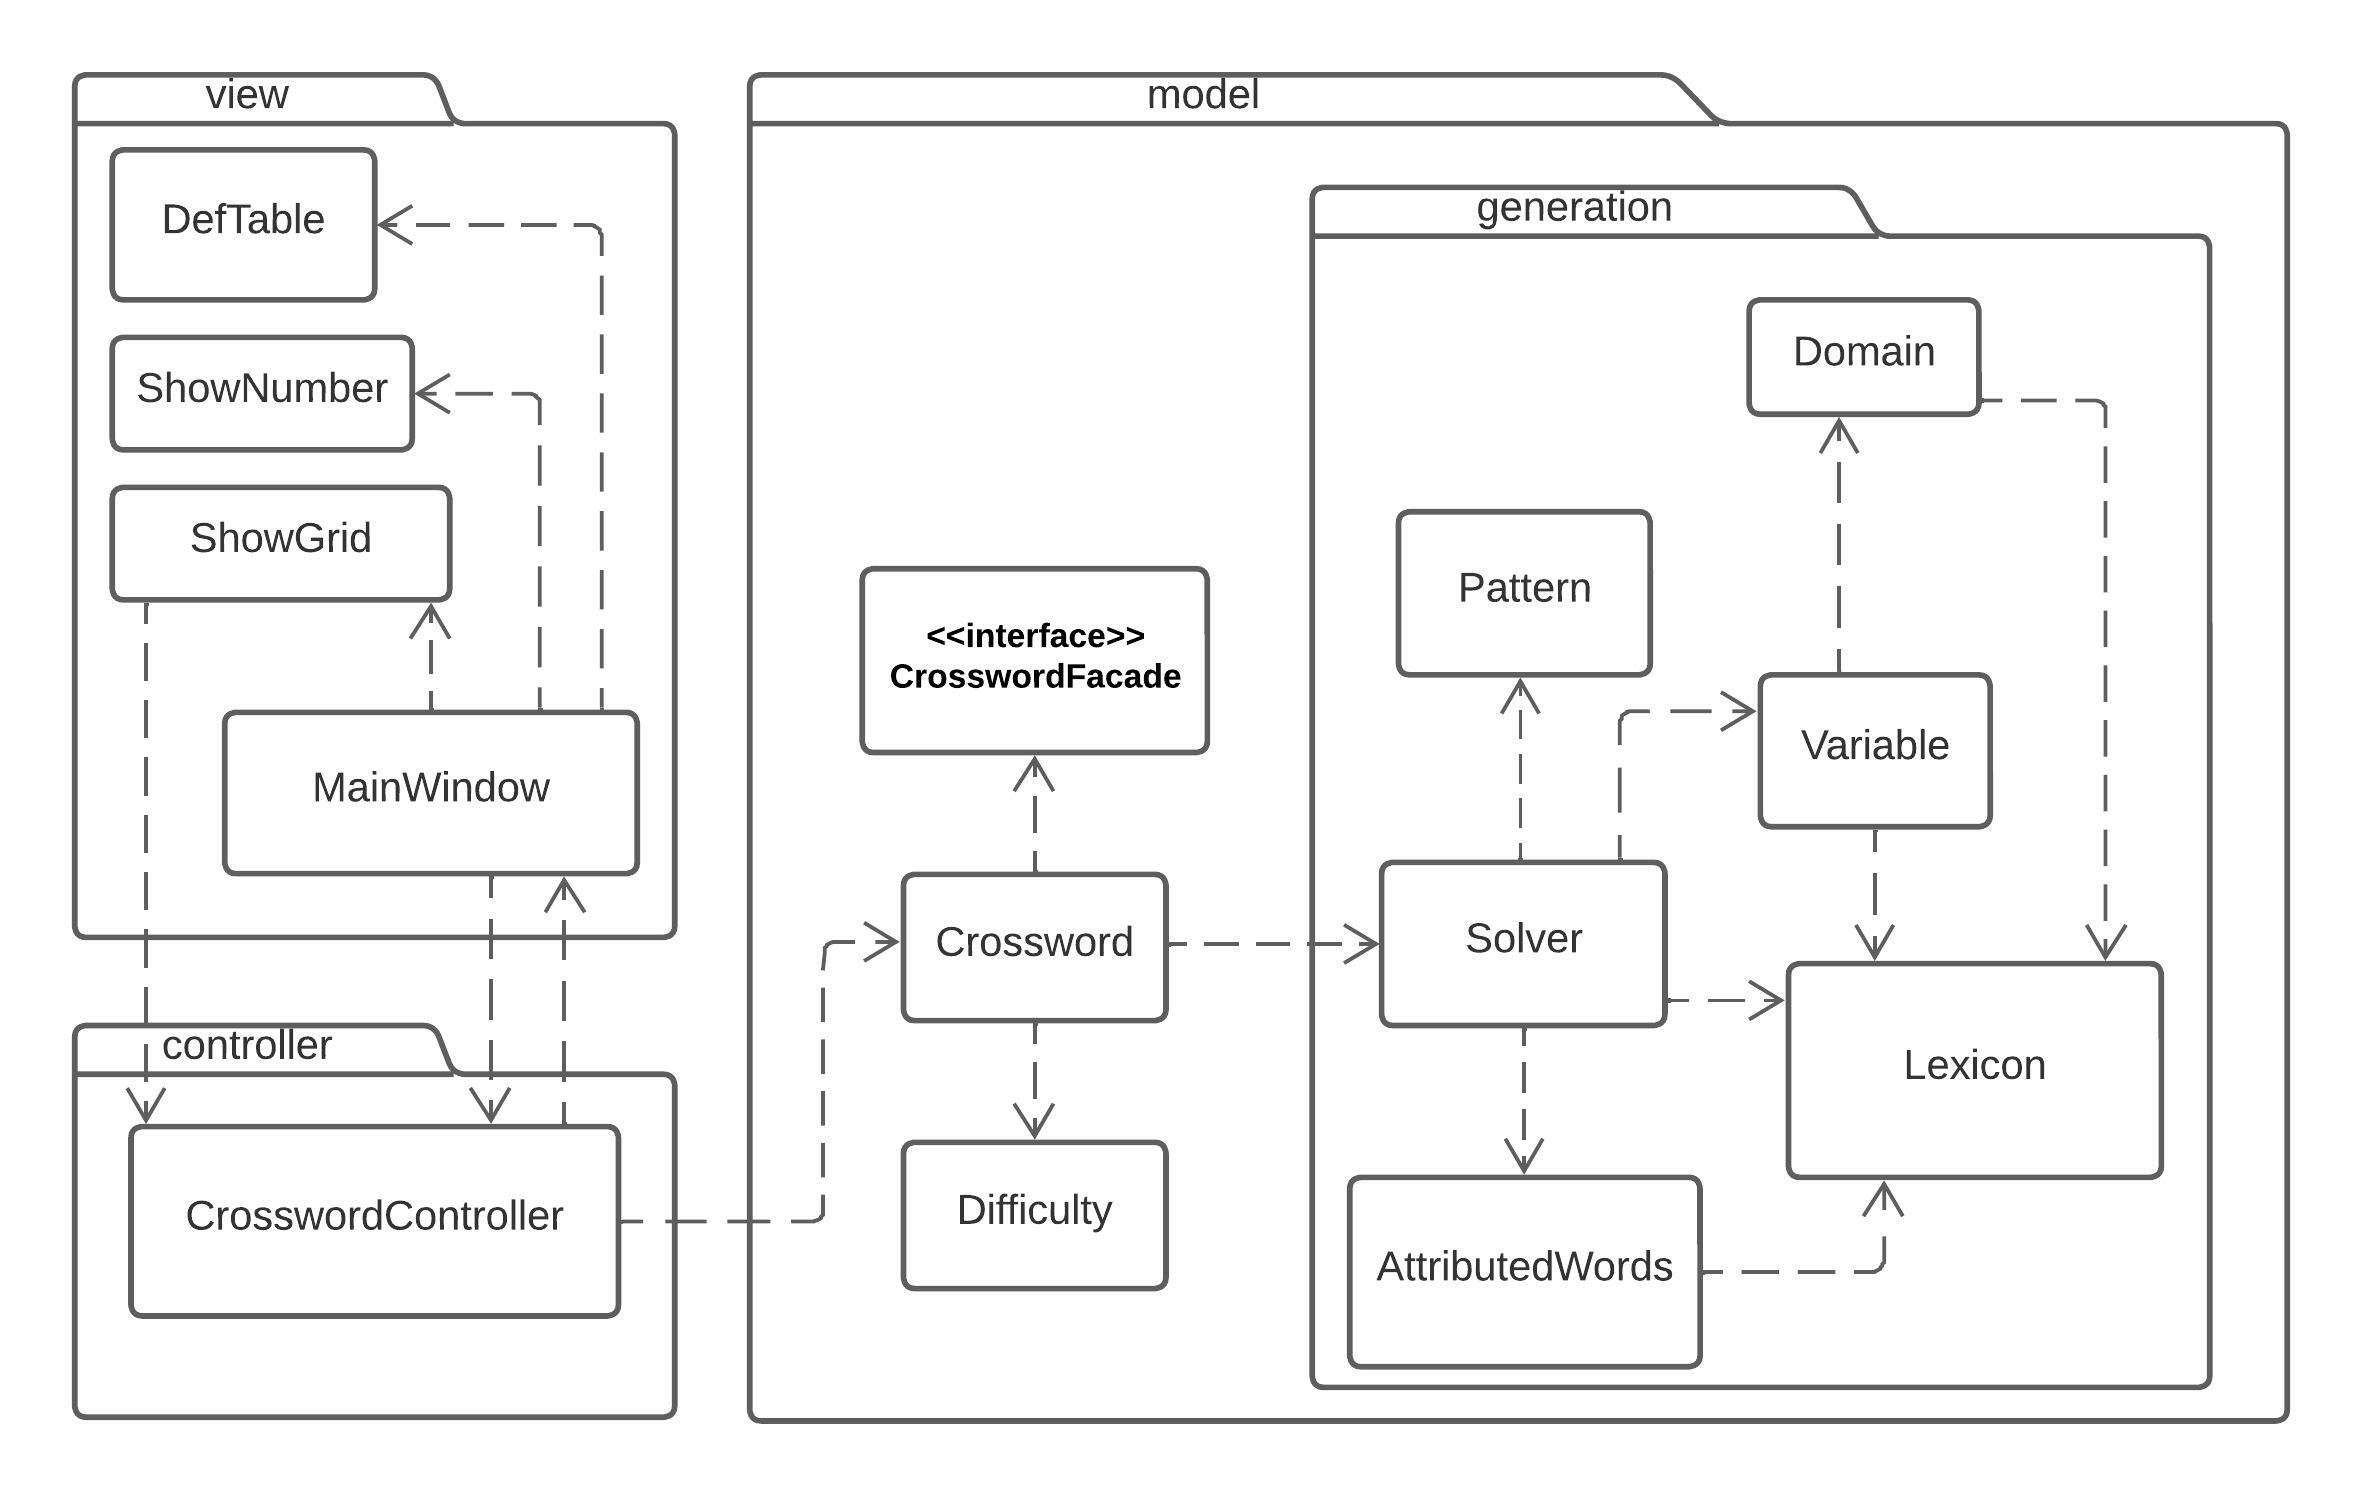
\includegraphics[width=1\linewidth]{diag_paquetages.jpeg}
    \caption{Diagramme de paquetages UML de notre application}
    \end{figure}
    Nous avons réparti les classes dans 3 paquetages principaux en se reposant sur notre utilisation du modèle MVC : un paquetage pour la \textbf{\textit{view}}, un pour le \textbf{\textit{controller}} et un pour le \textbf{\textit{model}}. Dans le \textbf{\textit{model}}, nous avons aussi voulu séparer le jeu de mots croisés, de la génération de grille en créant un paquetage \textbf{\textit{generation}} dans lequel nous avons mis toutes les classes concernant la génération d’une grille.
    
\section{Documentation du code}
Lors de la programmation, nous avons pris soin d’entièrement documenter notre code. Pour cette documentation nous avons utilisé le générateur de documentation \textbf{Doxygen} \cite{Dox}, cela à impliqué de commenter toutes nos classes, attributs et méthodes dans un format particulier qui permet donc aussi de lire la documentation directement sur le code.
\\\\
Pour générer la documentation html que \textbf{Doxygen} propose nous avons utilisé la commande :\\
\textbf{"doxygen Doxyfile"} dans le repertoire \textbf{\textit{"src/build"}}. \textit{Doxyfile} étant un fichier de configuration fournis par \textbf{Doxygen}, que nous avons modifié selon nos souhaits.
\\\\
Sur le dépôt de notre application, cette documentation se trouve dans le répertoire : \begin{center}\center\textbf{\textit{"data/doxygen\_documentation/html"}}\end{center}
En ouvrant le fichier \textbf{\textit{annotated.html}} vous ouvrez la page qui répertorie toutes les classes de notre implémentation, en cliquant sur une classe vous aurez accès à sa documentation (sous forme de page \textit{html}).
\begin{figure}[H] 
    \center 
    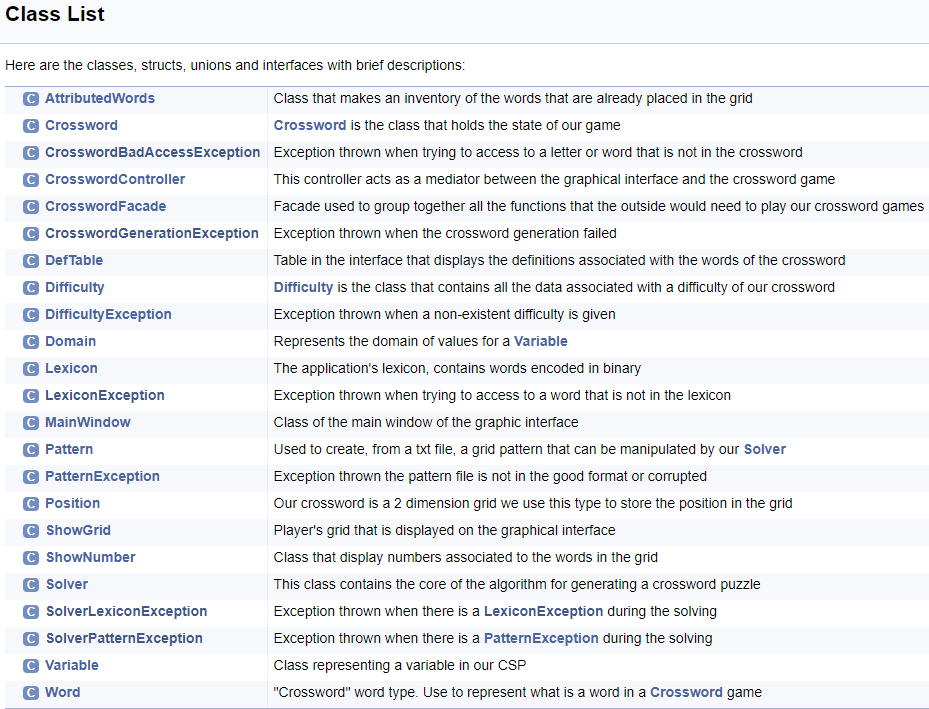
\includegraphics[width=1\linewidth]{doxygen.png}
    \caption{Page \textit{annotated.html} de la documentation}
\end{figure}

\newpage
\section{Résultat final}
Depuis l'écran d'accueil ci-dessous l'utilisateur peut séléctionner une difficulté ou importer une grille précédemment exportée :
\begin{figure}[H] 
 \center 
 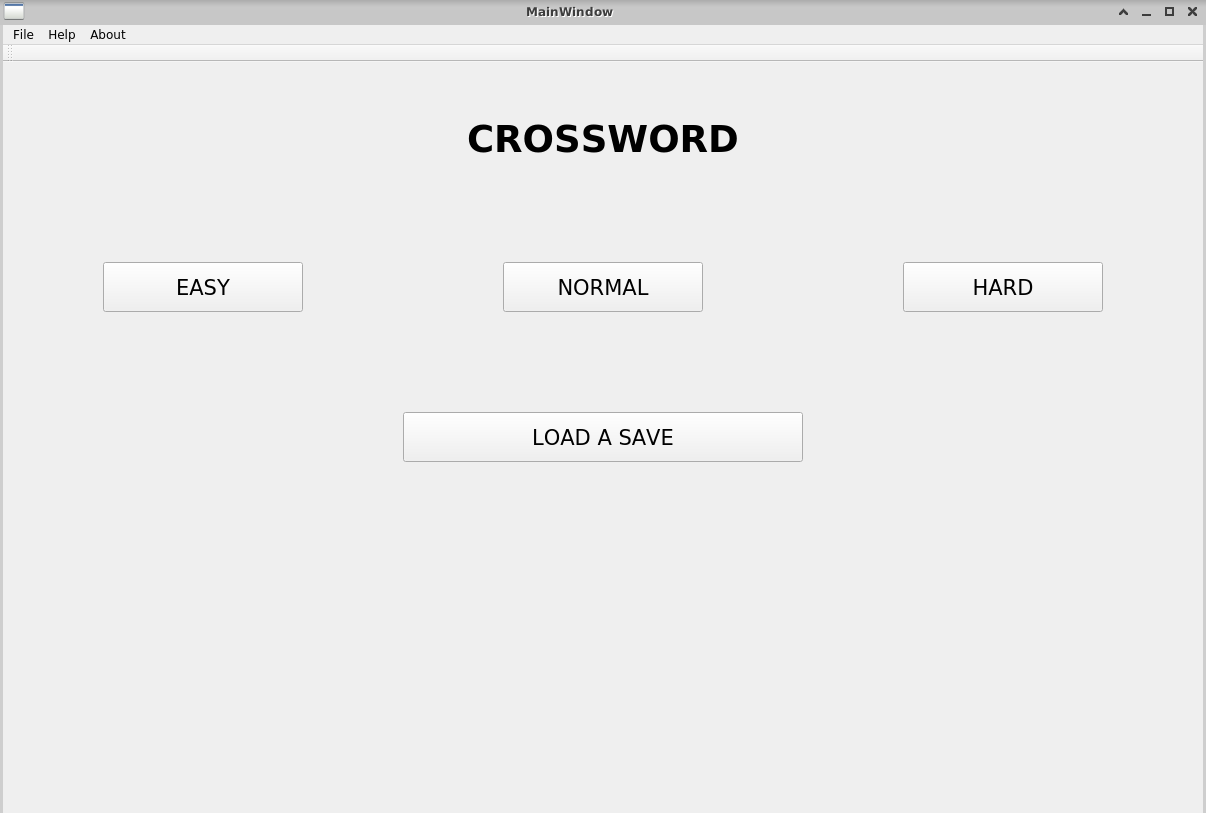
\includegraphics[height=3in]{resultats/menu.png}
 \caption{Menu de l'application}
 \end{figure}

Voici des exemples de résultats pour les trois niveaux de difficulté :

 \begin{figure}[H] 
 \center 
 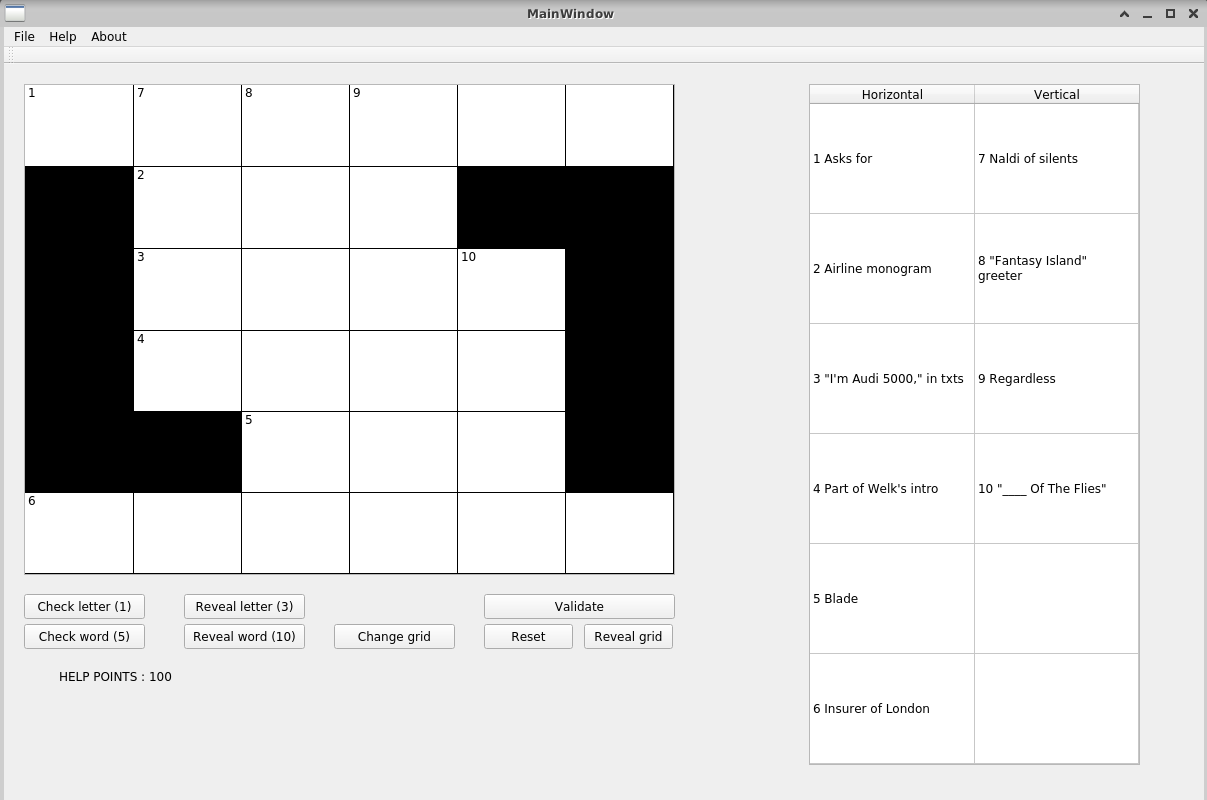
\includegraphics[height=3in]{resultats/easy_vide.png}
 \caption{Grille niveau facile vide}
 \end{figure}
 \begin{figure}[H] 
 \center 
 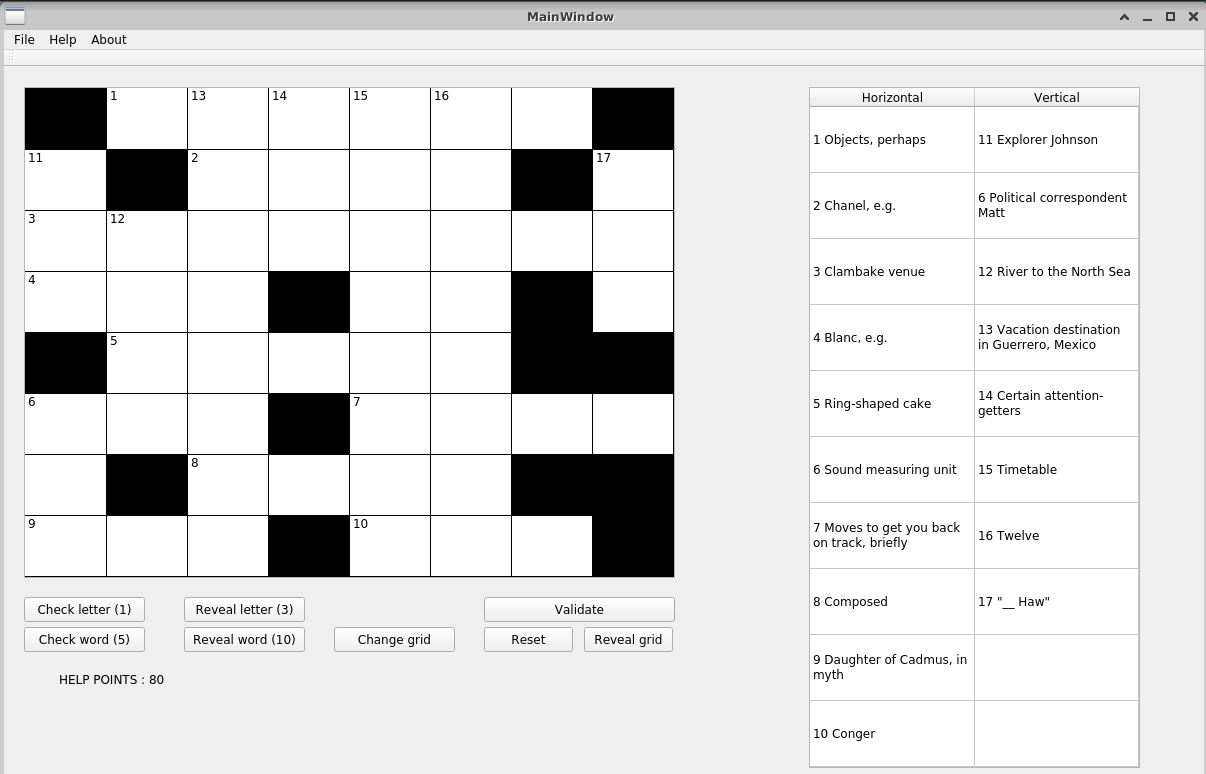
\includegraphics[height=3in]{resultats/normal_vide.png}
 \caption{Grille niveau normal vide}
 \end{figure}
  \begin{figure}[H] 
 \center 
 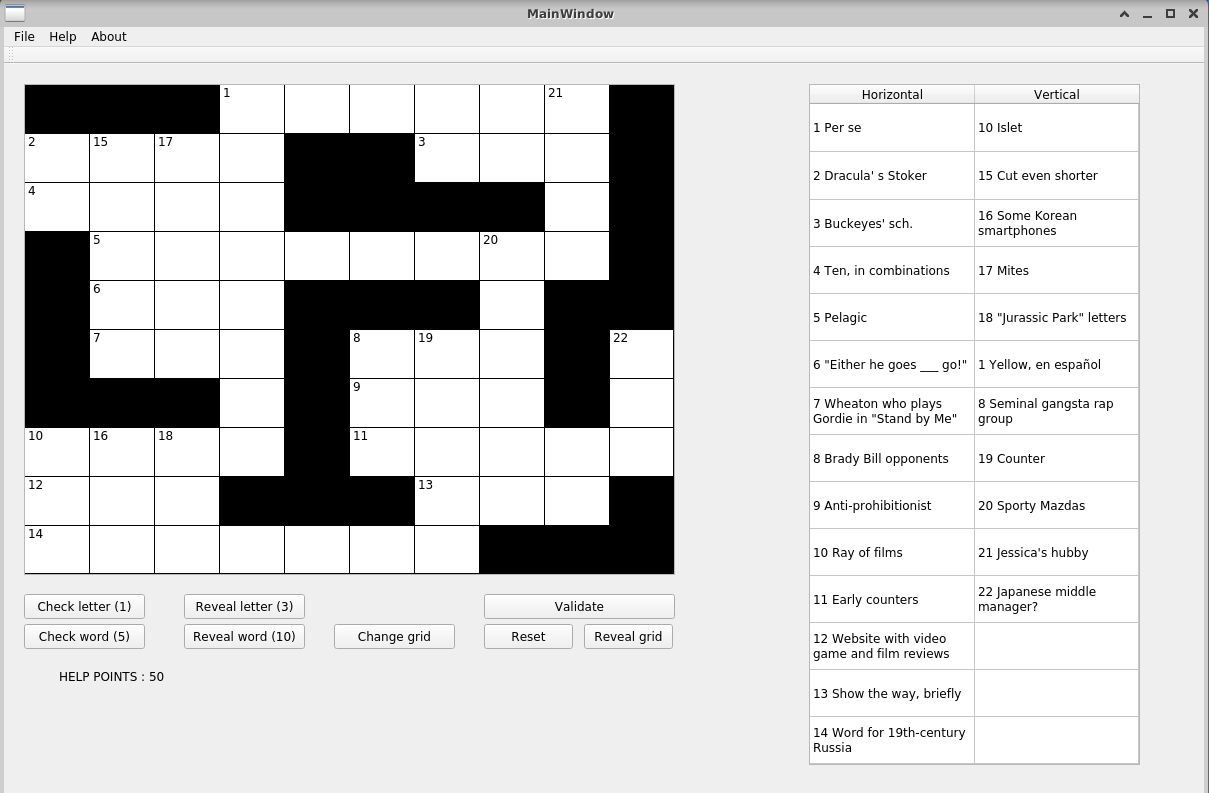
\includegraphics[height=3in]{resultats/hard_vide.png}
 \caption{Grille niveau difficile vide}
 \end{figure}
 
Lors de la partie l'utilisateur bénéficie de plusieurs aides. Il peut vérifier ou révéler une case ou un mot. Chaque aide coûte un certain nombre de points. L'utilisateur commence la partie avec un nombre de points d'aide plus ou moins élevé suivant le niveau de difficulté (cf. captures).
Pour vérifier ou révéler un mot, le joueur peut simplement sélectionner la définition du mot choisi et ensuite cliquer sur le bouton correspondant. Par exemple pour révéler un mot :
 \begin{figure}[H] 
 \center 
 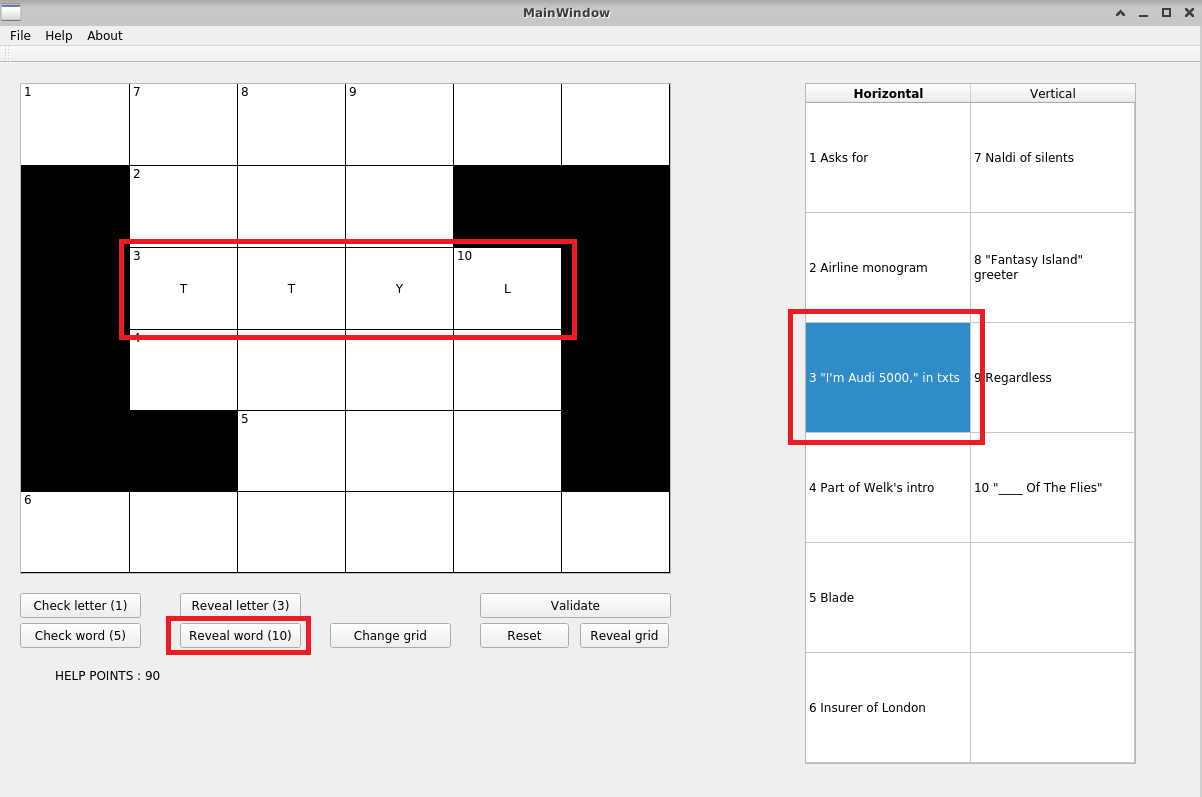
\includegraphics[height=3in]{resultats/easy_reaveal_word_2.png}
 \caption{Révéler un mot avec l'interface}
 \end{figure}

On voit que le nombre de points a été mis à jour et est maintenant de 90.
Pour vérifier ou révéler une lettre on procède de la même façon en sélectionnant cette fois-ci la case. \\

L'utilisateur peut choisir de dévoiler la grille à n'importe quel moment s'il souhaite abandonner. Il pourra aussi vérifier sa grille pour savoir si elle est correcte ou non.
 \begin{figure}[H] 
 \center 
 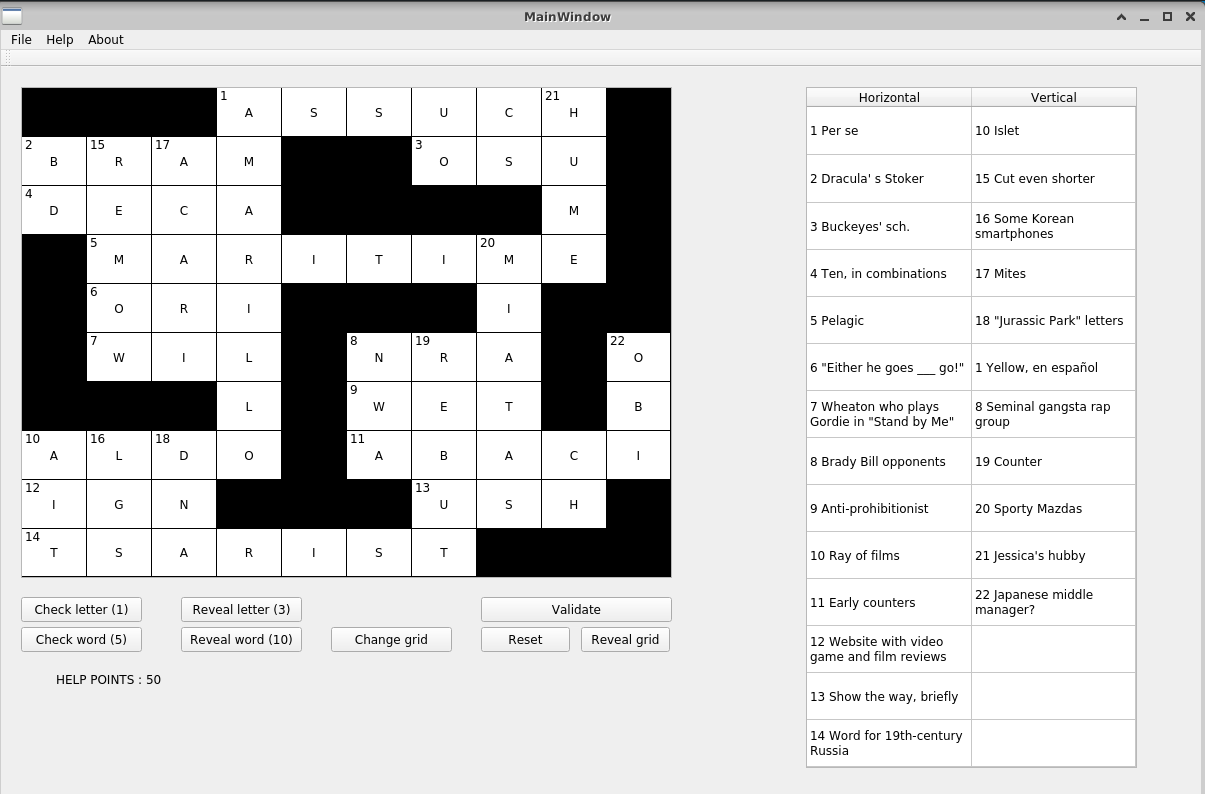
\includegraphics[height=3in]{resultats/hard_remplie.png}
 \caption{Grille niveau difficile révélée}
 \end{figure}

Nous pouvons également suivre l'exécution du solver en mode terminal et voir la grille s'afficher à chaque mot placé :
 \begin{figure}[H] 
 \center 
 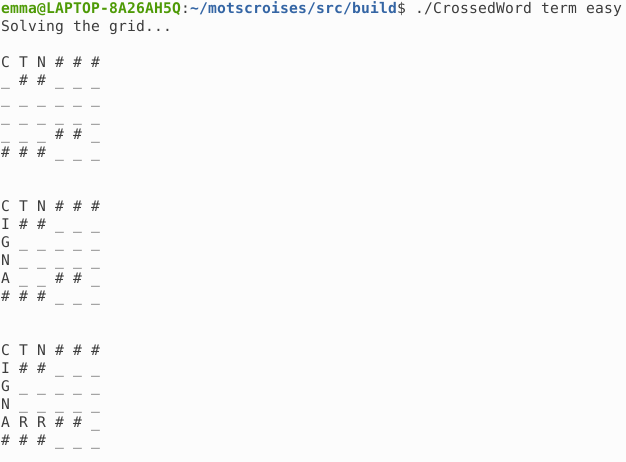
\includegraphics[height=3in]{resultats/terminal_1.png}
 \caption{Début du lancement en mode terminal}
 \end{figure}
  \begin{figure}[H] 
 \center 
 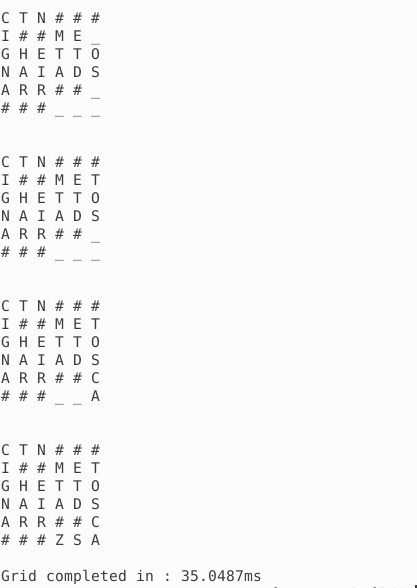
\includegraphics[height=3in]{resultats/terminal_2.png}
 \caption{Fin du lancement en mode terminal}
 \end{figure}

Cela nous a principalement servi durant le développement afin de surveiller le déroulement des exécutions.

\newpage

\section{Tests de génération de grilles sur des grilles de tailles variables}
    L'idée va être maintenant de faire une analyse la plus complète possible du logiciel. Pour cela, nous allons ici faire une description des tests que nous avons effectué. Ceux-ci ont pour objectif de convaincre que le logiciel développé se comporte correctement dans diverses situations (jugées "hors du commun"). \\
    
    Dans cette partie, nous allons confronter notre algorithme à des grilles aux dimensions variables, possédant pour certaines des cases noires, et pour d'autres uniquement des cases blanches (i.e des grilles vides). Pour chacune des générations, nous intégrerons une capture d'écran de la génération issue du solver, puis nous noterons le temps associé. A noter que les conditions de tests sont un ordinateur fixe tournant sous Ubuntu 20.04 avec 64 GO de RAM.

    \subsection{Sur des grilles carrées}
        \subsubsection{Avec cases noires}
        \begin{center}
    \begin{tabular}{ | c |  m{5cm} | m{5cm} | }
    \hline
    Affichage terminal & Paramètres \\ 
    \hline
      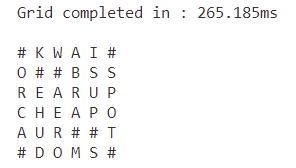
\includegraphics[]{easy 6_6 black.png}
    & dimension 6*6 \newline Pattern : easy2.txt\\
    \hline
    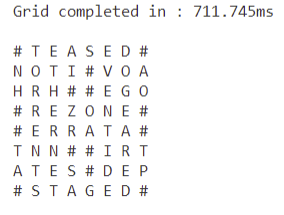
\includegraphics[]{medium 8_8 black.png}
    & dimension 8*8 \newline Pattern : medium1.txt\\
    \hline
    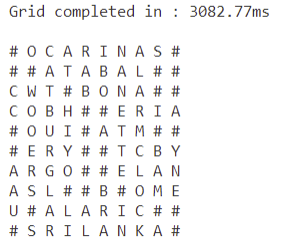
\includegraphics[]{hard 10_10 black.png}
    & dimension 10*10 \newline Pattern : hard1.txt\\
    \hline
    \end{tabular}
    \end{center}
    
    \subsubsection{Grilles vides}
    \begin{center}
    \begin{tabular}{ | c |  m{5cm} | m{5cm} | }
    \hline
    Affichage terminal & Paramètres \\ 
    \hline
      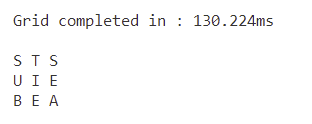
\includegraphics[]{3.png}
    & dimension 3*3 \\
    \hline
      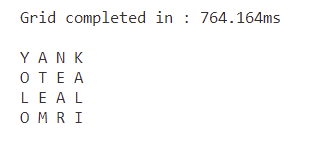
\includegraphics[]{4.png}
    & dimension 4*4 \\
    \hline
      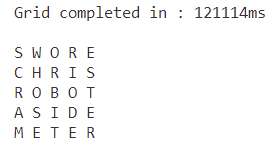
\includegraphics[]{5_5.png}
    & dimension 5*5 \\
    \hline
    \end{tabular}
    \end{center}
    \subsection{Sur des grilles rectangulaires} 
        \subsubsection{Avec cases noires}
        \begin{center}
    \begin{tabular}{ | c |  m{5cm} | m{5cm} | }
    \hline
    Affichage terminal & Paramètres \\ 
    \hline
      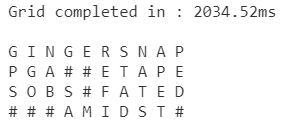
\includegraphics[]{10_4 black.png}
    & dimension 10*4 \newline Pattern : 10\_4.txt \\
    \hline
    \hline
      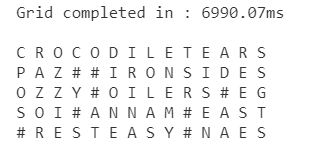
\includegraphics[]{14_5 black.png}
    & dimension 14*5 \newline Pattern : 14\_5.txt \\
    \hline
      
    \end{tabular}
    \end{center}
        \subsubsection{Grilles vides}
        \begin{center}
    \begin{tabular}{ | c |  m{5cm} | m{5cm} | }
    \hline
    Affichage terminal & Paramètres \\ 
    \hline
      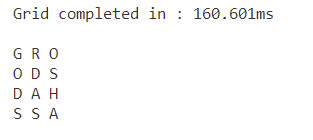
\includegraphics[]{3_4.png}
    & dimension 3*4 \\
    \hline
      \includegraphics[]{4_3.png}
    & dimension 4*3 \\
    \hline
      \includegraphics[]{5_4.png}
    & dimension 5*4 \\
    \hline
      \includegraphics[]{6_4.png}
    & dimension 6*4 \\
    \hline
    \end{tabular}
    \end{center}
        
    \subsection{Bilan du test de génération}
    
    Résumons ce que nous avons observé jusqu'ici, à travers les 2 histogrammes suivants :
    
    \begin{figure}[H] 
    \center 
    \includegraphics[width=0.7\linewidth]{grid_pattern.png}
    \caption{Temps de génération de grille avec des cases noires pré-placées}
    \end{figure}
    
    \begin{figure}[H] 
    \center 
    \includegraphics[width=0.7\linewidth]{grid_pattern_var.png}
    \caption{Temps de génération de grille sur des grilles vides aux dimensions variables}
    \end{figure}
    
    Au préalable, il est important de préciser que ces temps peuvent être globalement assez variables. En effet, notre algorithme intègre une part de \textbf{randomization} en ce qui concerne la recherche des mots. Afin d'être le plus précis possible, nous avons répété les expériences 3 fois et effectué une moyenne. Nous aurions pu faire le choix de désactiver cette randomisation pour les tests mais cela n'est pas représentatif de ce qu'il se passe réellement dans le coeur de l'algorithme et cela fausserait les résultats (on prendrait en effet toujours les premiers mots qui conviennent). \\
    
    Nous remarquons que sur des grilles où des cases noires sont pré-placées, les temps de génération de grilles sont largement acceptables puisqu'ils n'excédent pas les 4 secondes. C'est ce qu'atteste la figure 41. En revanche, sur des grilles vides, jusqu'à une taille de 5 x 5 nous avons un temps de génération convenable (de l'ordre de 30 secondes comme nous pouvons voir sur la figure 42). Par contre, à partir de 6 x 6, le temps de génération de la grille dépasse les 5 heures (nous n'avons réussi à terminer sa génération). Le temps de géneration croie de façon exponentielle.  Cela justifie le fait que nous avons préféré limiter le temps d'attente en ajoutant des cases noires sur la grille, comme énoncé précédemment. \\
    Aussi, notons que nos tests ont débuté avec une taille de 3 x 3 au minimum ; cela se justifie simplement par le fait que notre base de données ne possède pas de mots de taille inférieure. En revanche, l'utilisation d'une base de données possédant des mots de taille 1 et 2 ne poseraient pas de soucis à notre algorithme principal. \\
    
    \section{Un peu de combinatoire}
    
    \hspace*{0.6cm}Nous allons dans cette section parler de combinatoire dans l'objectif d'expliquer le comportement que nous avons observé en figure 42. En effet, il est important de comprendre en quoi la génération d'une grille de mots-croisés à partir d'une grille vide de taille 6 x 6 est si longue. Est-ce fatalement dû à la combinatoire et donc aux nombres de combinaisons exponentielle à explorer ? Ou est-ce dû à la base de donnée. C'est la réponse à laquelle nous allons essayer de répondre dans cette section. 
    
        \subsection{Complexité algorithmique}
        \hspace*{0.6cm} Restons sur le cas de la génération de la grille vide de taille 6 x 6, c'est d'abord celui-ci que nous devons élucider. 
        \newpage
        \subsubsection{Quelques chiffres}
        Sur une telle grille, sont présents : 
        \begin{itemize}
            \item \textbf{36} lettres, dont 20 sont situées à \textit{l'extérieur} de la grille et sont donc en relation avec 2 autres lettres (pour les 4 lettres situées sur les coins supérieurs droits et gauche (respectivement inférieur droits et gauches) ou en relation avec 3 autres lettres pour les autres. Les 16 autres lettres situées au milieu ont toutes 4 voisines. 
            
            \item \textbf{12} mots à placer qui bien sûr possèdent pour chacune de leur lettre une relation grammaticalement logique avec les 4 lettres qui les entourent $\rightarrow$ 12 variables à remplir selon notre définition des \textbf{variables}
            
            \item \textbf{7823} mots de taille 6 dans notre base de données
            
        \end{itemize}
        
        Ainsi, sans introduire d'aléas dans notre recherche algorithmique (en enlevant le mélange des mots que le solver introduit intialement), l'algorithme se comportera ainsi : pour chacune des variables de la grille, il y aura potentiellement \textbf{7823} possibilités. Aussi, pour chacune de ces variables, il faudra vérifier que chacune de ses lettres s'intersecte correctement avec : 
        
        \begin{itemize}
            \item 6 autres lettres pour les mots situés sur les extrêmités
            
            \item 12 autres lettres pour les autres variables
        \end{itemize}
        
        Simplifions les calculs : pour chacune des 12 variables, après placement d'un mot il faudra chercher parmi les \textbf{$7823 - n$} ($n$ étant le nombre de mots déjà placés sur la grille) mots de la base de données (en supposant qu'à chaque fois on doit parcourir tous les mots de la base de données de taille 6) un mot qui intersecte et respecte toutes les contraintes de voisinage. Ainsi, nous sommes à ce stade déjà sur une complexité de recherche très importante ($ > O(n^2) $). Rajoutons à cela que plus nous plaçons de mots sur la grille, plus les contraintes sont importantes, intuitivement nous le voyons simplement. \\
        
        Ainsi, à de très nombreux moments de l'algorithme, le solver place tous les mots sauf un puis se "rend compte" que le dernier mot à placer n'existe pas dans la base de données. Ainsi, il revient en arrière (par la technique utilisée, le \textbf{backtracking}) pour des fois revenir à une grille vide. Combien de combinaisons potentielles existent ? Nous avons un choix de 12 mots parmi 7823, un simple calcul nous donne une combinatoire égale à \textbf{108762005423896952721591306484241558583} ($10^{38}$ environ, rapellons que le nombre d'atomes dans l'univers est évalué à $10^{80}$) combinaisons possibles. Inutile de préciser que cela est plus qu'exponentiel. Bien sûr, il est illusoire de penser qu'on testera tout cela, mais potentiellement cela peut arriver et cela donne tout de même un ordre d'idée sur la complexité moyenne (même s'il est difficile de l'évaluer précisémment) en présence d'une telle base de mots. \\
        
        A ce stade, nous commencons à intuiter le fait que le temps de génération très important de la grille \textbf{6 x 6} ne vient pas de notre algorithme, mais plutôt de notre base de données. Pour le confirmer, nous allons effectuer des tests. \\
        
        \subsection{Tests avec une base de données de mots de taille 6 simplifiée}
        
        \hspace*{0.6cm} L'idée va être ici d'utiliser une base de donnée de mots de taille 6 , très simple, dont nous sommes sûrs que si notre algorithme est performant, il trouvera une solution (au moins). Dans notre cas, nous utiliserons la base de donnée composée des mots suivants (nous savons préalablement qu'ici le solver est censé trouver 2 grilles différentes) : {ACAPER, GAVOTE, IVERON, TINTIN, ETIOLE, SERRES, AGITES, CAVITE, AVENIR, PORTOR, ETOILE, RENNES}. Et sans trop de surprise, nous obtenons les 2 résultats suivants :
        
        \begin{figure}[H] 
            \center 
            \includegraphics[width=0.3\linewidth]{grid_1.png}
            \caption{Résultat avec une grille de 6 x 6 sur la base de données de test - possibilité 1}
        \end{figure}
        
        \begin{figure}[H] 
            \center 
            \includegraphics[width=0.3\linewidth]{grid_2.png}
            \caption{Résultat avec une grille de 6 x 6 sur la base de données de test - possibilité 2}
        \end{figure}
        
        Commande pour effectuer ce test : \\
        \textbf{./CrossedWord term test -p ../../data/patterns/tests/9\_8.txt \\ -bd ../../data/database/word\_database\_test.txt}.
        
        \subsection{Un premier bilan de complexité}
        
        D'abord, cela nous conforte à dire que notre algorithme est robuste et que le résultat observé en figure 42 était directement \textbf{corrélé} à la base de données dont était nourrie le solver. Ensuite, cela nous pousse à faire des tests sur des grilles vides de tailles plus importantes que 6 x 6, afin de poursuivre les tests de notre application. Ces tests, jusqu'alors impossibles (du moins dans un temps raisonnable) seront réalisés avec le même principe d'une base de donnée simplifiée, pour confronter la robustesse du logiciel à différentes tailles. \\
        
        Réalisons par exemple un test sur une grille (toujours vide), de taille \textbf{9 x 8}, avec la base de donnée simplifiée suivante : {DERAPERA, ECOTAMES, CONTRAIS, REFRACTE, OULIPIEN, CRASHERA, HANTERAS, ENTERAIS, STERASSE, DECROCHES, ECOEURANT, RONFLANTE, ATTRISTER, PARAPHERA, EMACIERAS, REITERAIS, ASSENASSE} dont nous savons qu'il existe une solution. Le solver arrive effectivement à résoudre la grille (dans un temps raisonnable) : \\
        
        \begin{figure}[H] 
            \center 
            \includegraphics[width=0.3\linewidth]{grid_3.png}
            \caption{Résultat avec une grille de 9 x 8 sur la base de données de test}
        \end{figure}
        
        Commande pour effectuer ce test:\\ \textbf{./CrossedWord term test -p  ../../data/patterns/tests/9\_8.txt \\ -bd ../../data/database/word\_database\_test.txt}. \\
        
        Ainsi, nous comprenons que notre algorithme est robuste. Il est par contre directement lié à la base de données : l'intuition nous le faisait savoir, nous en avons la certitude à travers cette batterie de tests effectuée ici. Néammoins, notre choix ne s'est pas orienté vers ce type de base de données. Bien qu'il permette une génération de grilles vides, il ne permet pas d'obtenir différentes grilles. D'un point de vue utilisateur, cela est moins attractif. Il serait possible de trouver un compromis en utilisant une base de donnée de taille inférieure mais les possibilités de grilles différentes seraient forcément réduites par rapport à notre base de donnée privilégiée. \\ \\
        
        Par ailleurs, à des fins expérimentales nous avons laissé la base de données de mots de tests utilisée ici, située à l'emplacement \textbf{data/database/word\_database\_test.txt}. \\
        
        Nous allons enfin généraliser cela sur des grilles vides plus grandes, toujours sur la base de données de tests, en faisant varier la taille des grilles. Notons que cette base de mots n'est utilisée qu'à des fins expérimentales : elle ne possède pas de définitions associées. De plus, les grilles supérieures à une taille de 10 seront réalisées à partir de grilles de mots mêlés ; les mots n'auront ainsi aucune signification, néammoins nous avons l'assurance qu'ils s'entremêlent tous, les uns avec les autres. Les résultats obtenus sont les suivants : 
        
        \begin{figure}[H] 
            \center 
            \includegraphics[width=0.7\linewidth]{Grid_time.png}
            \caption{Bilan de performances avec la base de données de test}
        \end{figure}
        
        La figure 46 vient conclure cette partie, qui nous a permis de nous conforter dans la robustesse et la performance de notre algorithme, conjointement à la base de mots, tous deux intimement liés. Notons pour finir que l'algorithme se comporte également bien sur des grilles de mots de taille supérieures. Etant donné leur faible fréquence d'apparition lexicale, nous avons décidé d'écarter ces mots. 
        
        \subsection{Tests avec des mots "parasites"}
        
        Bien sûr, les conditions expérimentales dans lesquelles nous avons effectué les tests ci-avant sont idéales. Idéales dans le sens où pour chacune des tailles de grilles, elles ne contiennent que des mots qui peuvent former une solution. Nous allons à ce stade, toujours dans le but de tester notre application (mais cette fois en condition un peu plus réaliste) rajouter quelques mots parasites pour chacune des tailles et observer l'impact sur le temps de génération de la grille. Ainsi, créeons une nouvelle base de données, située dans data/database/word\_database\_test\_parasite.txt. Pour chacune des dimensions étudiées sur des grilles vides (cf figure 6, taille 6x6, 9x8, 12x12 et 14x14), nous allons ajouter 500 mots parasites (issus de la base de donnée principale). Observons ci-après les résultats : 
        
        \begin{figure}[H] 
            \center 
            \includegraphics[width=0.7\linewidth]{test_parasite.png}
            \caption{Bilan de performances avec la base de données de test (avec mots "parasites")}
        \end{figure}
        
        Nous observons que les temps sont plus importants que sans mots "parasites" (cf figure 27), en revanche ils restent tout à fait raisonnable (de l'ordre de la seconde). De plus, ils permettent de générer plusieurs grilles, ce qui était manquant avec la base de donnée de test. Cela est ainsi plus réaliste, mais les possibilités de grilles en sorties restent toutefois limitées. 
        
    
    \section{Combinatoire, une fatalité sans issue ?}
    Nous avons exposé en section précédente les tenants et aboutissants de la complexité et (surtout) de la combinatoire associée à nos algorithmes. Finalement, cette phase de tests nous a apporté de l'intuition. Bien entendu, nous ne pourrons pas violer un problème \textbf{NP-Complet} en espérant une complexité linéaire, ce serait illusoire. En revanche, nous pouvons accélérer certains traitements. C'est ce que nous avons du moins intuité en observant notre algorithme se dérouler durant cette importante partie de tests. 
    
    \subsection{Quelques améliorations apportées}
        \subsubsection{Coût de l’application d’une contrainte}
            Pour rappel, une contrainte sur une variable dans notre problème correspond formellement à: \guillemotleft  la variable doit avoir la  \textbf{lettre} \textit{n} à la \textbf{position} \textit{x}\guillemotright. 
            \\\\
            La méthode que nous avions donc utilisée jusqu’ici se déroulait en plusieurs étapes:
            \begin{itemize}
                \item Parcourir le lexique en regroupant dans un \textbf{ensemble \textit{N}} tous les mots qui ont la \textbf{lettre} \textit{n} à la \textbf{position} \textit{x};
                \item Considérons \textbf{\textit{D}}: le domaine d’une variable. Nous allons ensuite effectuer une intersection $\textbf{\textit{N}} \cap \textbf{\textit{D}}$;
                \item Cette intersection devient le nouveau domaine de la variable, nous avons uniquement gardé les mots du domaine qui ont la \textbf{lettre} \textit{n} à la \textbf{position} \textit{x};
            \end{itemize}
            
            Nous avions remarqué que cette méthode étais très coûteuse, il y a d’abord un parcours du lexique entier (dans notre cas 30 000 opérations) puis l’intersection de deux domaines qui, dans notre contexte, demande d’appliquer l’intersection sur chaque lettre de chaque mot (ce qui donne un nombre d’opération d’environ: \textbf{nombre de mots} de taille \textit{k}  dans le lexique * la \textbf{taille} \textit{k}). Nous arrivions très vite à des centaines de milliers d’opérations à chaque fois que nous souhaitions appliquer une contrainte à une variable, cette opération étant le cœur de notre algorithme cela coûte très cher à la performance de notre générateur.
            \\\\
            L’optimisation que nous avions mis en place pour réduire ce coût est de ne plus passer par le lexique pour appliquer les contraintes. Nous parcourons directement le domaine de la variable concernée en regardant sur chaque mot directement la lettre qui se trouve à la \textbf{position} \textit{x} et si cette lettre n’est pas la \textbf{lettre} \textit{n}, le mot est enlevé du domaine. Ce qui nous donne, pour une variable de \textbf{taille} \textit{k}, un nombre d’opération qui est d’environ le nombre de mots de \textbf{taille} \textit{k}  dans le lexique. Ce qui dans notre cas est au maximum $\cong6500$.
        \subsubsection{Mots appliquant la même contrainte sur une variable bloquée}
            Pour rappel, lors de la génération d’une grille, le backtracking \guillemotleft se déclenche\guillemotright   lorsqu’une variable n’a plus de valeur possible: on revient donc en arrière et change le mot précédent en espérant que les contraintes appliquées par le nouveau mot ne bloquent plus la variable concernée.
            \\\\
            Lors des tests nous avons remarqué que beaucoup de mots été placés pour rien, par exemple : le mots MANGER vient d’être placé et la variable qui passe par le 'M' du mot MANGER n’a plus de valeur possible, l’algorithme revient donc en arrière et change MANGER par MANIER. La variable concernée se voit réappliquer la contrainte (la lettre ‘M’ à la \textbf{position} \textit{x}) qui l’a bloqué précédemment. A ce moment là nous perdions beaucoup de temps à tester des mots lors du backtracking que nous savions déjà \guillemotleft mauvais\guillemotright.
            \\\\
            La solution a donc été de détecter au moment du backtracking le cas où le mot qui vient d’être placé à appliqué une contrainte qui a bloqué une variable : si c’est le cas nous récupérons la \textbf{position} \textit{x} et la \textbf{lettre} \textit{n} du mot qui a bloqué la variable victime, et nous enlevons tous les mots qui ont cette lettre à cette position, dans le domaine de la variable qui a posé la contrainte problématique.
        \subsubsection{Les résultats suites aux modifications apportées}
            \underline{Note :} Pour cette partie, nous utiliserons la base de données d'origine, celle de taille 31316. \\
            
            
            Nous espérons des résultats améliorés en comparaison avec ceux obtenus en figure 23. Afin de mieux se rendre compte des (éventuels) changements, nous réaliserons les expériences sur les grilles où les temps étaients les plus importants, à savoir : 
            
            \begin{itemize}
                \item 6*4 : 5000 ms
                \item 5*5 : 7500 ms
                \item 6*5 : 40 000 ms
            \end{itemize}
            
            Les nouveaux résultats sont les suivants : 
            \begin{itemize}
                \item 6*4 : 1500 ms
                \item 5*5 : 3500 ms
                \item 6*5 : 17 000 ms
            \end{itemize}
            
            Nous constatons qu'avec les quelques modifications apportées, nous gagnons un facteur 2 à 3 en moyenne pour les grilles étudiées ce qui n'est pas négligeable. A ce stade, nous ne voyons plus d'améliorations significatives qui pourraient nous faire gagner du temps sans changer l'architecture globale du projet. Nous pensons avoir mené l'efficacité à bout des algorithmes. 
    \newpage
    \section{Tests aux frontières - limites de l'application}
    
        \subsection{Conditions d'expériences}  
            Notre programme est capable de générer des grilles de très grandes tailles, nous avons voulu mesurer les limites de ces grilles en temps et en mémoire. Pour cela, nous avons sélectionné une grille difficile, il s'agit de hard5.txt, que nous avons dupliquée jusqu'à la dimension désirée. Une grille générée de 100*100 est disponible dans "data/misc/screen\_test\_grilles".
            \\\\
            Concernant les valeurs obtenues dans ces tests, elles sont une approximation grâce à un calcul de moyenne des valeurs obtenues. En effet de par le processus de randomisation, il est difficile d'obtenir des résultats fiables. Retirer cette randomisation ne nous permettrait pas de résoudre certaines grandes grilles ou alors bien moins efficacement.
            \\\\
            Il faut également prendre en compte que les résultats suivants dépendent essentiellement du pattern qui a été choisi ici. Il est possible par exemple de pouvoir générer des grilles bien plus grandes sur des patterns différents où par exemple, on aurait un nombre plus faible de Variables et de contraintes. De plus, ces tests utilisent la base de données de notre application, on pourrait donc imaginer de meilleures performances sur ce type de grille avec une base de données plus adaptée.
                    
        \subsection{Limites en temps} 
            Pour mesurer le temps pris par notre application, nous avons cette fois-ci fait le choix d'y inclure également le temps pris par notre algorithme de création des variables en plus de celui du solveur. En effet, lorsque nous ne traitons pas des grilles "blanches", le nombre de contraintes et de variables n'est pas aussi important et ainsi le temps pris par l'algorithme de création de variable n'est alors plus si négligeable. Il reste néanmoins plutôt court, mais sur des grandes grilles, il est plus aisé de constater sa proportion par rapport au temps total.
            
            \begin{figure}[H] 
                \center 
                \includegraphics[width=0.9\linewidth]{tests_temps_grandes_grilles.jpg}
                \caption{Bilan de performances en temps sur des grandes grilles}
            \end{figure}
            
            On remarque que le temps pris par notre algorithme augmente bien de façon exponentielle, ainsi au bout d'une certaine dimension, il devient complétement impossible de pouvoir générer une grille dans un temps de l'ordre de la minute. Nous avons pu obtenir quelques grilles de dimensions 110*110 grâce à un comportement favorable de la randomisation en une trentaine de secondes, mais ce côté aléatoire de l'algorithme nous empêche de pouvoir obtenir des mesures fiables. La plupart des autres essais ont échoué en dépassent des dizaines de minutes.
        
        \subsection{Limites en mémoire}
            Dans le cas théorique où nous pourrions générer des grilles plus grandes que celles des tests précédents, nous aurions eu une autre limite : celle de la mémoire occupée par les variables que nous manipulons dans notre algorithme. Dans le graphique suivant, on a associé à ces mêmes grilles leur nombre de variables, cela représente le nombre de mots que peut contenir la grille sur de telles dimensions. Nous avons alors pu lancer le processus de génération de grilles en l'arrêtant juste après la phase de création des variables pour étudier l'espace mémoire occupé.
        
            \begin{figure}[H] 
                \center 
                \includegraphics[width=0.9\linewidth]{tests_mémoire_grandes_grilles.jpg}
                \caption{Bilan de performances en mémoire sur des grandes grilles}
            \end{figure}
        
            Sur la machine de test, cette grille de 300*300 est très proche de la limite de ce qu'on pourrait être amené à générer. En effet, une telle grille nécessiterait une quantité de 12 Go destinée uniquement au stockage de ces variables. D'après les calculs, nous estimons qu'une variable nécessite en moyenne 0,5 Mo. Cela est conséquent, car nous avons besoin de sauvegarder de nombreux mots au sein d'une variable. Cependant, lors d'une utilisation classique que nous proposons, on ne manipule pas plus d'une trentaine de variables et ainsi, nous avons besoin de seulement 10 à 15 Mo au maximum pour le bon fonctionnement du programme. Nous aurions pu travailler sur une version différente de notre algorithme permettant ainsi d'allouer et de libérer ces variables au fur et à mesure de leurs utilisations, cela afin de pouvoir traiter des grilles plus conséquentes. Cependant, au vu des priorités de notre application, nous n'avons pas jugé cela utile, car dans l'utilisation de notre programme, ces limites étant bien hautes, nous ne sommes jamais bloqués par cette contrainte d'espace mémoire.
            
            \newpage
        
    \section{Tests concernant la base de données}
    
    Notre algorithme d'encodage de la base de données permet une intégration facile de toute autre base de données dans notre logiciel. En effet, il suffit de transformer toute autre base de donnée en un fichier d'extension \textbf{.txt} en classant les mots par taille et récursivement au sein de chaque taille par ordre alphabétique (en utilisant par exemple les librairies \textit{numpy} et \textit{pandas} fournies par \textbf{Python}). Ainsi, toute autre base de donnée présentée sous ce format là serait intégrée de manière transparente à notre logiciel. Pour rendre notre logiciel plus complet, nous pourrions intégrer un outil d'encodage pour convertir des bases de données existantes en des bases de données \textbf{compatibles} avec notre logiciel. Cela pourrait faire d'ailleurs partie des ajouts complémentaires à réaliser. \\
    
    Par contre, il est de la responsabilité de l'utilisateur de la base de données que sa base soit la plus complète possible. En effet, rappelons que notre base de données est issue d'une vraie base de mots croisés contenant des mots très courants et les plus faciles possibles à placer. C'est en effet de la diversité de la base de données que provient l'efficacité algorithmique résultante. En effet, une base de données contenant peu de mots ou des mots difficiles à placer (contenant par exemple peu de \textbf{voyelles}) entraînera un ralentissement important de l'algorithme voir une non résolution de la grille. \\
    
    A ce propos, nous allons effectuer des tests utilisant diverses tailles de bases de données, afin de montrer le comportement de notre logiciel selon ce point. Pour ce faire, nous allons utiliser la grille suivante : \\
    
    \begin{figure}[H] 
    \center 
    \includegraphics[width=0.7\linewidth]{bdd_pattern.png}
    \caption{Grille témoin utilisée pour les mesures de variation de taille de la base de données}
    \end{figure}
    
    Ce choix de grille pour ce test a été fait car elle présente des mots de tailles variables s'entremêlant à beaucoup de positions variées. \\
    \newpage
    Voici les résultats : \\
    
    \begin{figure}[H] 
    \center 
    \includegraphics[width=0.7\linewidth]{bdd.png}
    \caption{Comparaison de performances sur la grille témoin - variation de la taille de la base de données}
    \end{figure}
    
    Nous observons des résultats conformes à ce que l'intuition nous disait. Ceux-ci sont valables dans le cas où la randomization reste activée, ce qui est le cas ici, autrement nous aurions au contraire des résultats meilleurs. Ce test a pour seule vocation de nous conforter à garder une diversité des mots la plus importante, tout en conservant des performances convenables d'un point de vue utilisateur. \\
    
    Le bilan que nous faisons ici est que nous avons fais un compromis entre performance et diversité de génération des grilles. Nous avons préféré garder une base de donnée la plus diversifiée soit-elle mais ne pas proposer des grilles vides pour l'utilisateur. C'est ce qui nous a semblé être plus réaliste. En effet avec des grilles vides et dans un temps raisonnable nous n'aurions pu proposer que des grilles de dimensions 5 x 5, ce qui n'utilise pas au mieux notre base de données et qui n'est pas très agréable pour l'utilisateur en terme de diversité produite et donc d'expérience de jeu. Rappelons qu'initialement le but est bien sûr de produire une application logicielle pour un utilisateur, elle doit donc être la plus attractive possible. Neammoins, cette phase de tests nous a permis de confronter notre application à divers comportements et à diverses bases de données et cela nous a permis de voir (notamment) qu'il est possible de produire des grilles vides en temps tout à fait correct avec une base de données de mots plus adéquate. Les grilles sont par contre moins diversifiées, raison pour laquelle notre application native ne l'utilisera pas. Néammoins, un développeur pourra intégrer cette fonctionnalité très facilement. 

\newpage
\section{Tests unitaires}
\subsection{Choix de l'outil de test}
Après s'être renseignés sur internet sur les différents outils de test compatibles avec le language C++, nous avons decidé d'utiliser la librairie de GoogleTest \cite{Gt}, qui dispose d'une grande popularité et d'une bonne maintenabilité.

\subsection{Implémentation}
Chacun de nos tests est appliquée à une fonctionnalité précise de notre application et permet de s'assurer du bon fonctionnement de nos fonctions.\\
Pour leurs implementations, nous avons réutilisé les tests initialement associés aux besoins tout en ayant adapté leur utilisation à l'implementation finale de notre application.
\\
Voici la liste des tests que nous avons implementé :\\

\textbf{Tests positifs} : 
\begin{itemize}
    \item Bon fonctionnement de la difficulté choisie (paramètres de dimension et du nombre de points).
    \item Bon fonctionnement des boutons ("Reveal grid", "Check letter", "Check word", "Validate", "Reset grid").
    \item Bon fonctionnement du décompte du système de points lors de l'utilisation des aides.
    \item Ecriture d'une lettre appartenant à [a-zA-Z].
    \item Importation d'une grille (sera utilisé en tant qu' Oracle dans la plupart des tests).
    \item Exportation d'une grille.
\end{itemize}

\textbf{Tests négatifs} : 
\begin{itemize}
    \item Importation d'un fichier non existant ou corrompu.
    \item Ecriture d'une lettre n'appartenant pas à [a-zA-Z].
\end{itemize}




\newpage
\section{Gestion de projet}

\hspace{0.6cm}Afin de gérer ce projet, il a été important d'adopter une coopération d'équipe la plus importante possible. De manière générale, nous nous sommes organisés par subdivisions, souvent en sous-groupes de 2 ou 3, sur des tâches bien précises. Nous avons fait attention à ce que les tâches réalisées en parallèles n'aient pas besoin les unes des autres afin d'éviter tout conflit lors des regroupements de code. \\

Pour la partie technique, bien sûr, nous avons utilisé un dépôt Git (fourni par le Cremi, \textbf{GitLab}). Nous avons régulièrement organisé des sessions de code durant lesquelles nous avons pu travailler tous ensemble grâce à Visual Studio Live Share. \\

Aussi, nous avions un groupe Discord nous permettant de faire des réunions de manière régulière, soit planifiée, soit dès lors que le besoin s'en faisait ressentir. Cela nous a permis d'avancer de manière concertée vers ce que nous souhaitions. \\

Nous avons commencé l'implémentation du code assez tardivement dans le calendrier : nous avons en effet préféré prendre un peu plus de temps pour bien comprendre les différents PDF et ainsi avoir une idée la plus claire possible avant de commencer à coder. Cela nous a semblé important d'avoir une idée claire concernant le coeur algorithmique et sur le mode d'encodage de la base de données, qui sont les deux points primordiaux pour que le projet se déroule le mieux possible. 

\subsection{Outils utilisés}
Voici les différents outils que nous avons utilisés tout au long du projet :
\begin{itemize}
    \item Discord pour communiquer entre membres du groupe
    \item Balsamiq Mockup pour le maquettage
    \item Lucidchart pour les diagrammes
    \item Overleaf pour la rédaction commune des documents
    \item LibreOffice Calc pour la réalisation des graphiques
    \item Trello pour suivre les différentes tâches à réaliser et les répartir
    \item Google Drive pour le partage de documents
    \item Git/GitLab pour partager et versionner le code lors du développement de l’application
    \item Visual Studio Live Share pour coder en groupe 
\end{itemize}

\newpage
\section{Conclusion}

\subsection{Bilan technique} 
Dans l'ensemble notre application atteint les objectifs que nous nous étions fixés lors de la description des besoins. Nous sommes satisfaits de nos résultats, notre application est fonctionnelle. Comme prévu l'utilisateur peut jouer depuis une interface graphique qui est simple d'utilisation et il existe un mode terminal à l'intention des développeurs. La génération des grilles est rapide et notre programme ne requiert aucune connexion internet. Tout a été écrit et codé en anglais. \\

Il reste cependant quelques fuites de mémoire que nous n'avons pas réussi à identifier et régler. 

Nous pouvons aussi noter que nos fichiers base de données qui sont au format txt rendent l'utilisation de l'application sur windows compliquée, si le projet est cloné sur windows : le fichier de la base de données n'est plus utilisable par notre application.\\

Enfin, notre utilisation de Qt est peu désirable car nous avons utilisé qu'une seule fenêtre sur laquelle on cache et/ou affiche tous les composants tour à tour.\\
 

\subsection{Ce qu'on a fait, pas fait} 
En reprenant notre diagramme des cas d'utilisation initial : les besoins "Lancer la génération d'une grille", "Changer de grille", "Choisir un niveau de difficulté", "Jouer", "Exporter en txt", "Choisir une aide", "Valider la grille" et "Manipuler la grille" ont été implémentés. En revanche, les besoins "Choisir un thème", "Exporter en jpeg" et "Exporter en pdf" n'ont pas été implémentés par manque de temps. De plus, ces besoins avaient été classés comme des besoins conditionnels ou optionnels lors de la rédaction de notre cahier des besoins. Nous avons tout de même réalisé l'export en fichier JSON car permettre au moins un moyen d'export nous paraissait important. \\

Contrairement à ce que nous avions imaginé au début nous n'affichons pas non plus le nombre d'erreurs lorsque l'utilisateur valide la grille, il saura informé si la grille qu'il a remplie est correcte ou non. \\

Tous les besoins que nous avions classés comme essentiels ont été implémentés. Nous avons donc globalement atteint notre vision initiale de l’application.\\

\subsection{Perspectives et améliorations}
Comme décrit plus haut nous avons créé des fichiers texte à la main pour représenter les grilles contenant les cases noires déjà placées. Cela nous a permis notamment d'éviter de laisser la possiblité d'avoir des mots de taille deux sur la grille (notre base de données de mots possibles contient des mots de taille entre trois et quatorze). Des améliorations possibles seraient d'ajouter des mots de deux (et pourquoi pas de 1) à notre base de données ainsi que de pouvoir générer aléatoirement les grilles avec les cases noires qui seront ensuite résolues. \\

Notre façon de créer les variables pourrait aussi être améliorée car actuellement sur des grandes grilles qui contiennent donc beaucoup de variables nous passons un temps assez conséquent pour la création des variables. Il est même arrivé sur certaines résolutions de prendre plus de temps pour cette création qu'à résoudre la grille.\\

Enfin, l'utilisation de Qt pourrait être améliorée : actuellement il n'existe qu'une seule vue qui efface et ré affiche tous les composants à chaque changement. Il serait préférable de créer plusieurs vues, une pour chaque partie de l'application. \\

\subsection{Bilan global}
Ce projet nous a appris à fonctionner en groupe de taille assez conséquente puisque nous avons du travailler à six pour la première fois. Nous avons beaucoup appris autant en informatique qu’en organisation, conduite de projet et communication au sein d’un groupe. Nous avons bien fonctionné ensemble, nous avons beaucoup communiqué et bien réparti les tâches. Nous nous sommes tous investis dans ce projet et sommes contents de notre travail même si nous avons encore en tête des choses que l’on pourrait améliorer.


\newpage
\printbibliography
\newpage
\section{Nos vraies motivations pour la réalisation de ce solver}
Pour finir sur une touche humoristique, nous avons réalisé cette application pour aider un des plongeurs de l'équipe, spécialisé en résolution de mots croisés sous-marins. Le voici, en pleine action, début avril, dans les profondeurs du bassin d'Arcachon : 

\begin{figure}[H] 
                \center 
                \includegraphics[width=0.9\linewidth]{GOPR0248.JPG}
                \caption{Etude algorithmique en milieu aquatique}
\end{figure}

\begin{figure}[H] 
                \center 
                \includegraphics[width=0.9\linewidth]{Capture d’écran du 2022-04-21 20-20-41.png}
                \caption{Des performances \textbf{largement} inférieures à celles de notre solver}
\end{figure}

Pour découvrir l'aventure en vidéo, rendez-vous  \href{https://www.youtube.com/watch?v=NRIJIo-rFTw&feature=youtu.be}{ici} . 


\end{document}